% BEGIN GENERAL INFORMATION
\subsection{General information}
\begin{frame}
	\frametitle{Proton Accelerator at Paul Scherrer Institute (PSI)}
	\begin{itemize}
		\setlength{\itemsep}{\fill}
		\item High Intensity Proton Accelerator (HIPA) at PSI (Cyclotron)
		\item \SI{590}{\mega\electronvolt} proton beam with beam current up to \SI{2.4}{\milli\ampere} (\SI{1.5e16}{protons\per s})
		\begin{itemize}
			\vspace*{4pt}
			\item \SI{\sim1.4}{\mega\watt} \ra most powerful proton accelerator in the world
		\end{itemize}
		\vspace*{4pt}
		\item only two comparable accelerators
		\begin{itemize}
			\vspace*{4pt}
			\item TRIUMF in Vancouver (\SI{\sim0.25}{\mega\watt})
			\item LAMPF in Los Alamos (\SI{\sim0.8}{\mega\watt})
		\end{itemize}
% 		\item LHC takes \SI{28}{\minute} to accelerate a full injection (\SI{\sim0.2}{\mega\watt})
	\end{itemize}
	\begin{figure}
		\centering
		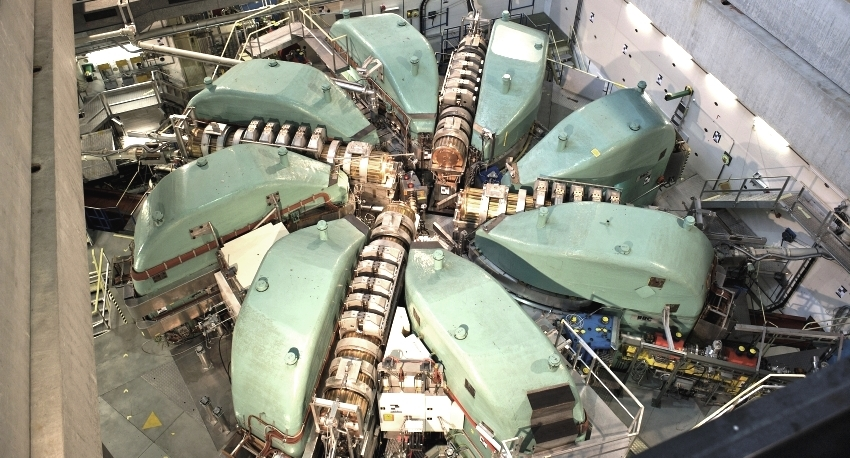
\includegraphics[width=6.5cm]{cyclotron}
	\end{figure}
\end{frame}
% ============================ new frame ==========================================>
\begin{frame}
	\frametitle{Beam line at Paul Scherrer Institute (PSI)}
	\begin{minipage}[c][.75\textheight]{6.5cm}
		\begin{itemize}
			\setlength{\itemsep}{\fill}
			\item using beam line $\uppi$M1 with \SI{260}{\mega\electronvolt\per c} positive pions ($\uppi^+$)
			\item tunable particle fluxes from \SI{2}{\kilo\hertz\per cm^2} to \SI{10}{\mega\hertz\per cm^2}
		\end{itemize}
		\begin{figure}
			\centering
			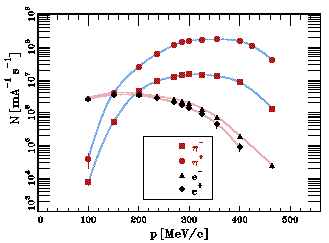
\includegraphics[width=5cm]{pim1}
		\end{figure}
	\end{minipage}
	\begin{minipage}{4.5cm}
		\begin{figure}
			\centering
			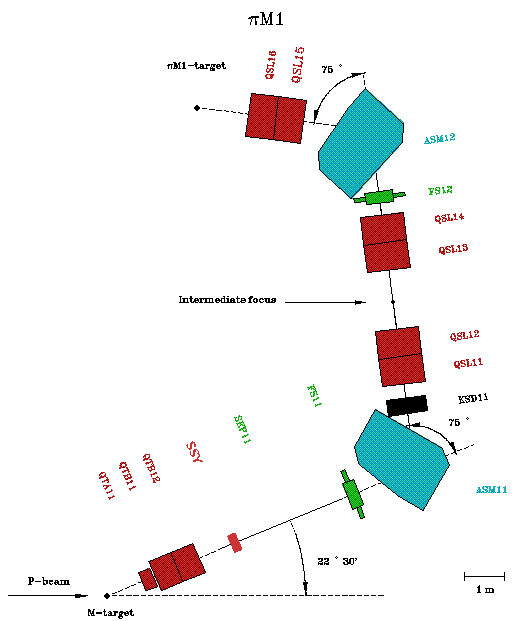
\includegraphics[width=5cm]{bpim1}
		\end{figure}
	\end{minipage}
\end{frame}
% ============================ new frame ==========================================>
\begin{frame}
	\frametitle{Measurements}
	\begin{itemize}
		\item performing several beam tests starting in $2013$
		\item using a modular self-built beam telescope with two possible setups:
			\begin{itemize}
				\item pad setup (testing whole diamonds as single pad detector)
				\item pixel setup (testing diamond sensors implanted on CMS-Pixel Chips)
			\end{itemize}
		\item investigating several materials and devices
		\begin{itemize}
			\item scCVD pad detectors (reproduce rate effect)
			\item pCVD pad and pixel detectors
			\item very first 3D pixel detector
		\end{itemize}
		\item studying non-irradiated and irradiated devices (up to \SI{1e16}{neq\per cm^2})
	\end{itemize}
	\begin{figure}
		\centering
		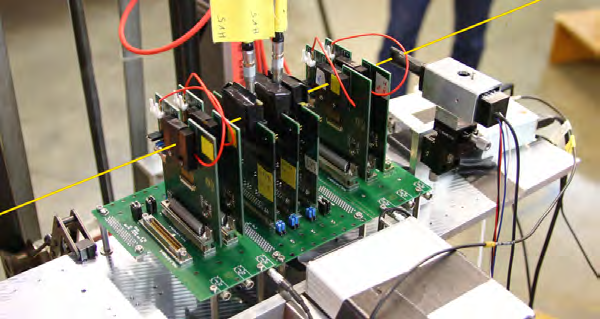
\includegraphics[width=6cm]{pad}
	\end{figure}
\end{frame}
% ============================ new frame ==========================================>
% END
% BEGIN SETUP
\subsection{Setup}
\begin{frame}
	\frametitle{Setup}
	\begin{figure}
		\centering
		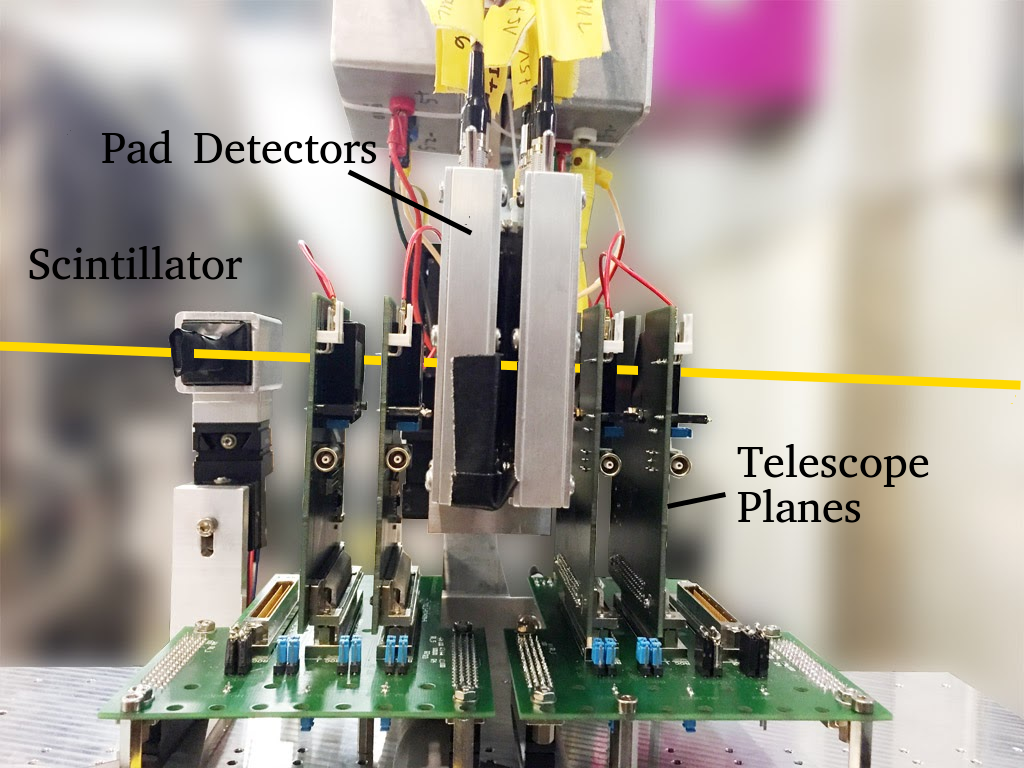
\includegraphics[width=5.5cm]{Setup}
	\end{figure}
	\begin{itemize}
		\setlength{\itemsep}{\fill}
		\item 4 tracking planes with analogue CMS pixel chips \ra provide scalable trigger
		\item 2 diamond pad detectors
		\item scintillator for precise trigger timing: sigma of \SI{1.3\pm.1}{ns}
		\item resolution: \SI{\sim80x50}{\micro\meter}
	\end{itemize}
\end{frame}
% ============================ new frame ==========================================>
\begin{frame}
	\frametitle{Schematics}
	\begin{figure}
		\centering
		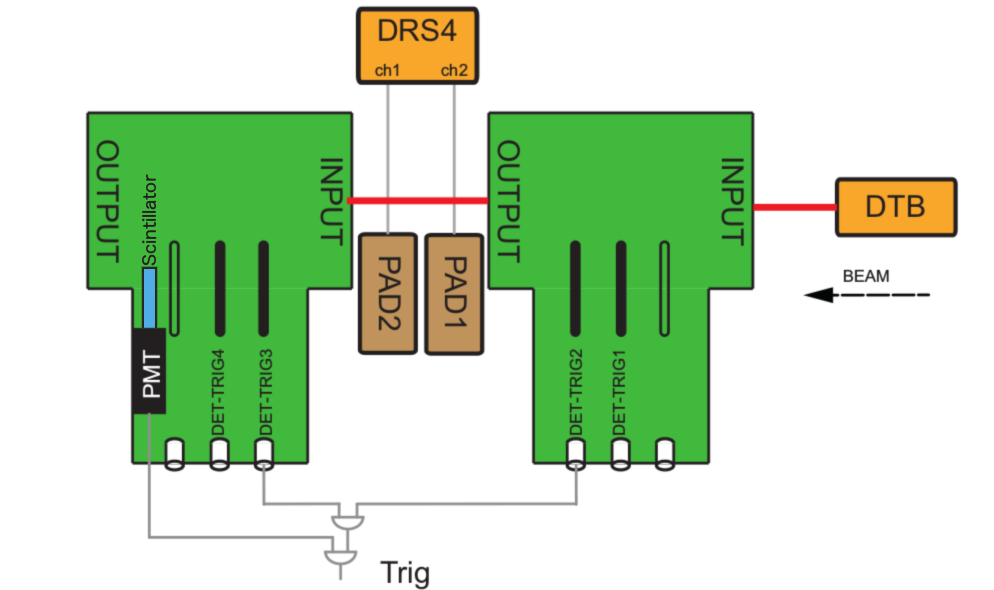
\includegraphics[width=7cm]{SchematicsV2}
	\end{figure}
	\begin{itemize}
		\setlength{\itemsep}{\fill}
		\item using PSI DRS4 Evaluation Board as digitizer for the pad waveforms
		\item using Digital Test Board (DTB) and pXar software for the telescope readout
		\item global trigger as coincidence of fastOR self trigger and scintillator signal
		\item EUDAQ as DAQ framework
	\end{itemize}
\end{frame}
% ============================ FRAME 16 ==========================================>
\begin{frame}
	\frametitle{Trigger Logic}
	\begin{minipage}[c][.5\textheight]{4cm}
		\begin{itemize}
			\setlength{\itemsep}{\fill}
			\item complicated trigger logic
			\item long setup time
			\item error prone
			\item varying cable length
		\end{itemize}
	\end{minipage}
	\begin{minipage}{8cm}
		\begin{figure}
			\centering
			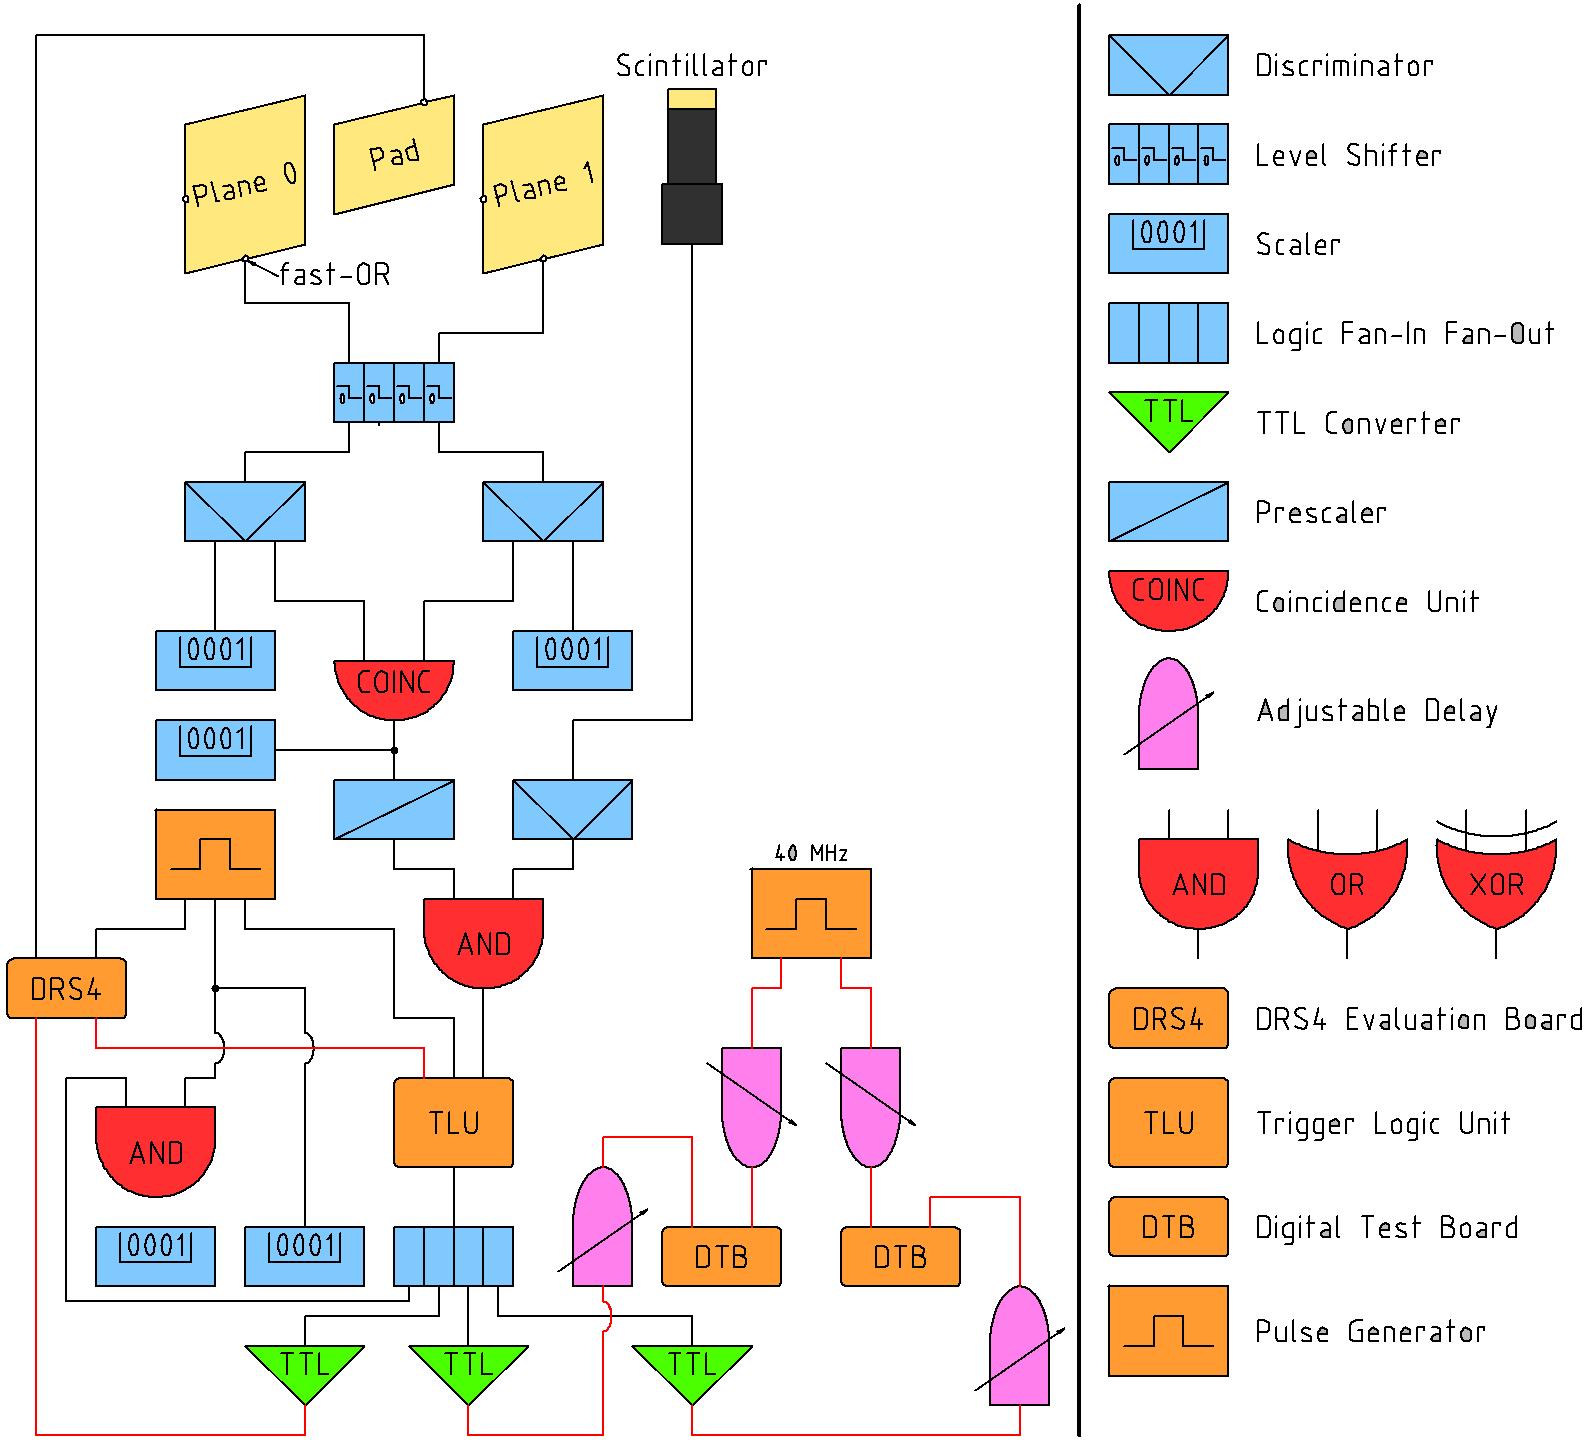
\includegraphics[width=7cm]{TrigLog}
		\end{figure}
	\end{minipage}
\end{frame}
% ============================ new frame ==========================================>
\begin{frame}
	\frametitle{DAQ}
	\begin{figure}
		\centering
		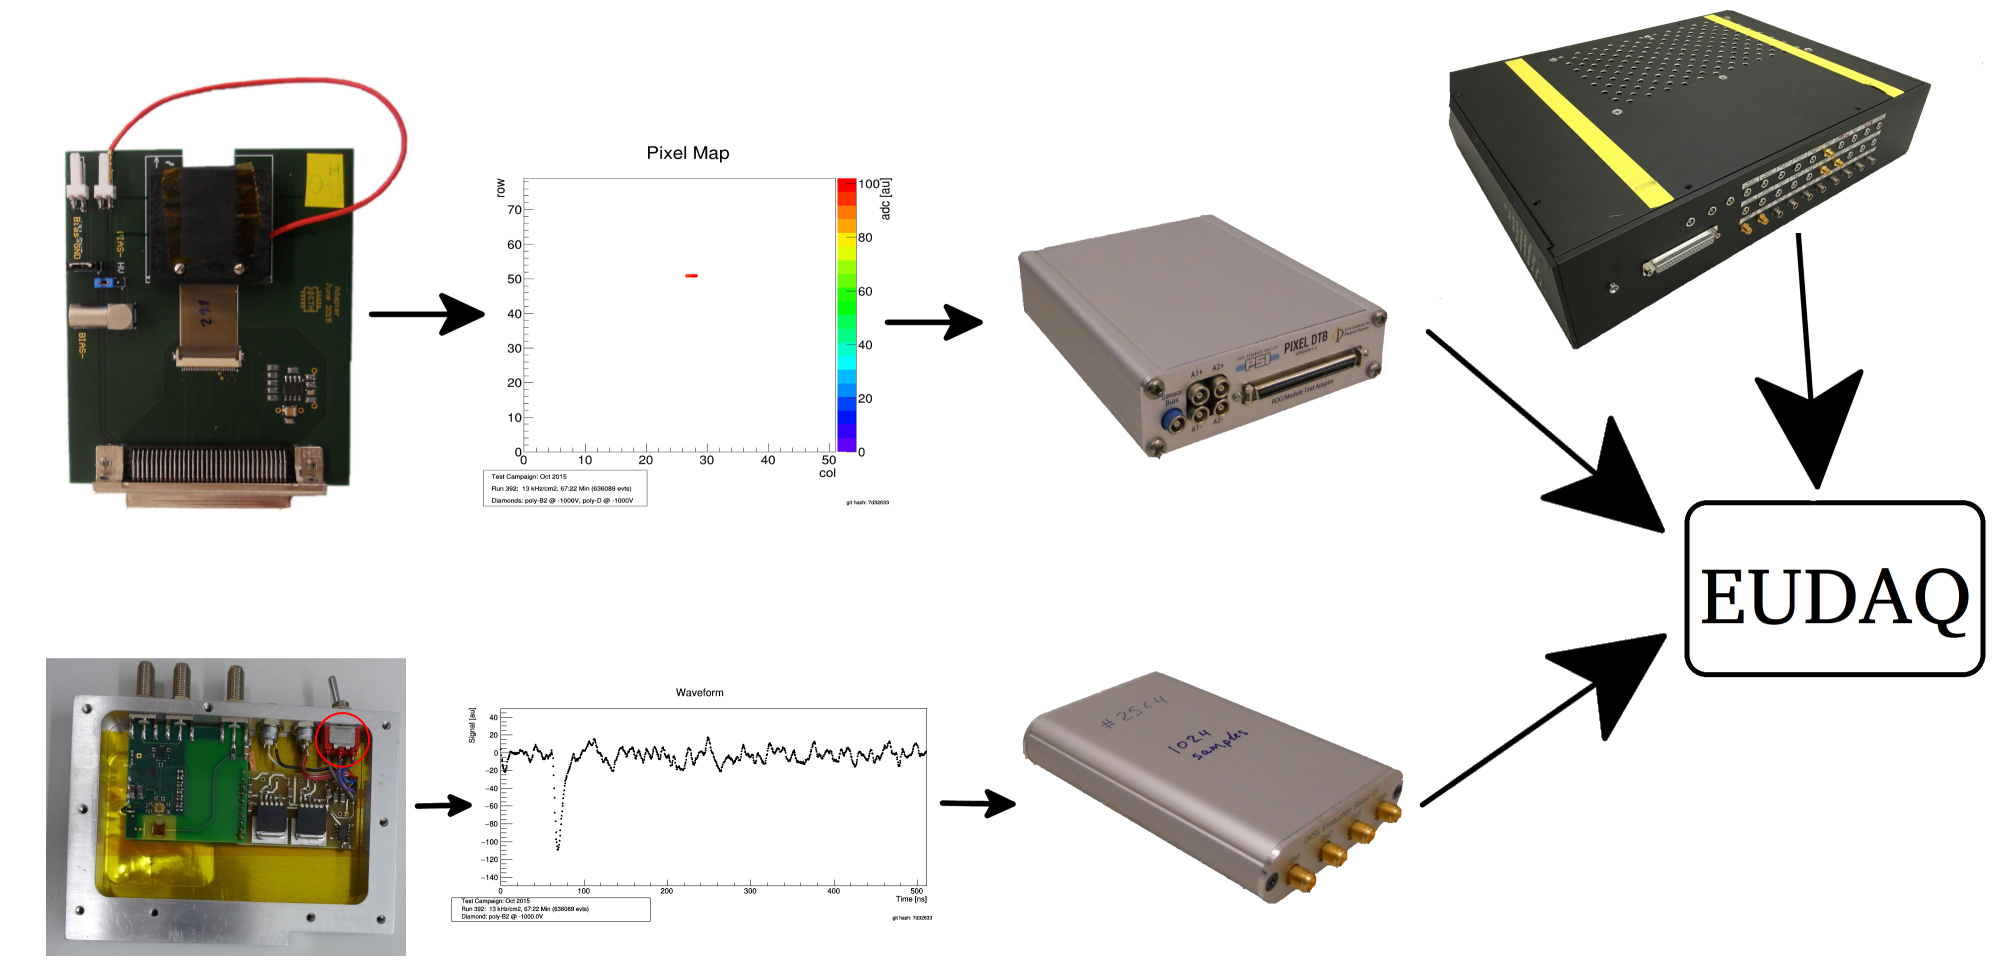
\includegraphics[width=.8\textwidth]{Intro}
	\end{figure}
	\begin{itemize}
		\item trigger unit to provide global trigger for all devices
		\item saving event based data stream as binary file using EUDAQ
	\end{itemize}
\end{frame}
% ============================ new frame ==========================================>
\begin{frame}
	\frametitle{Trigger unit (TU)}
	\begin{figure}
		\centering
		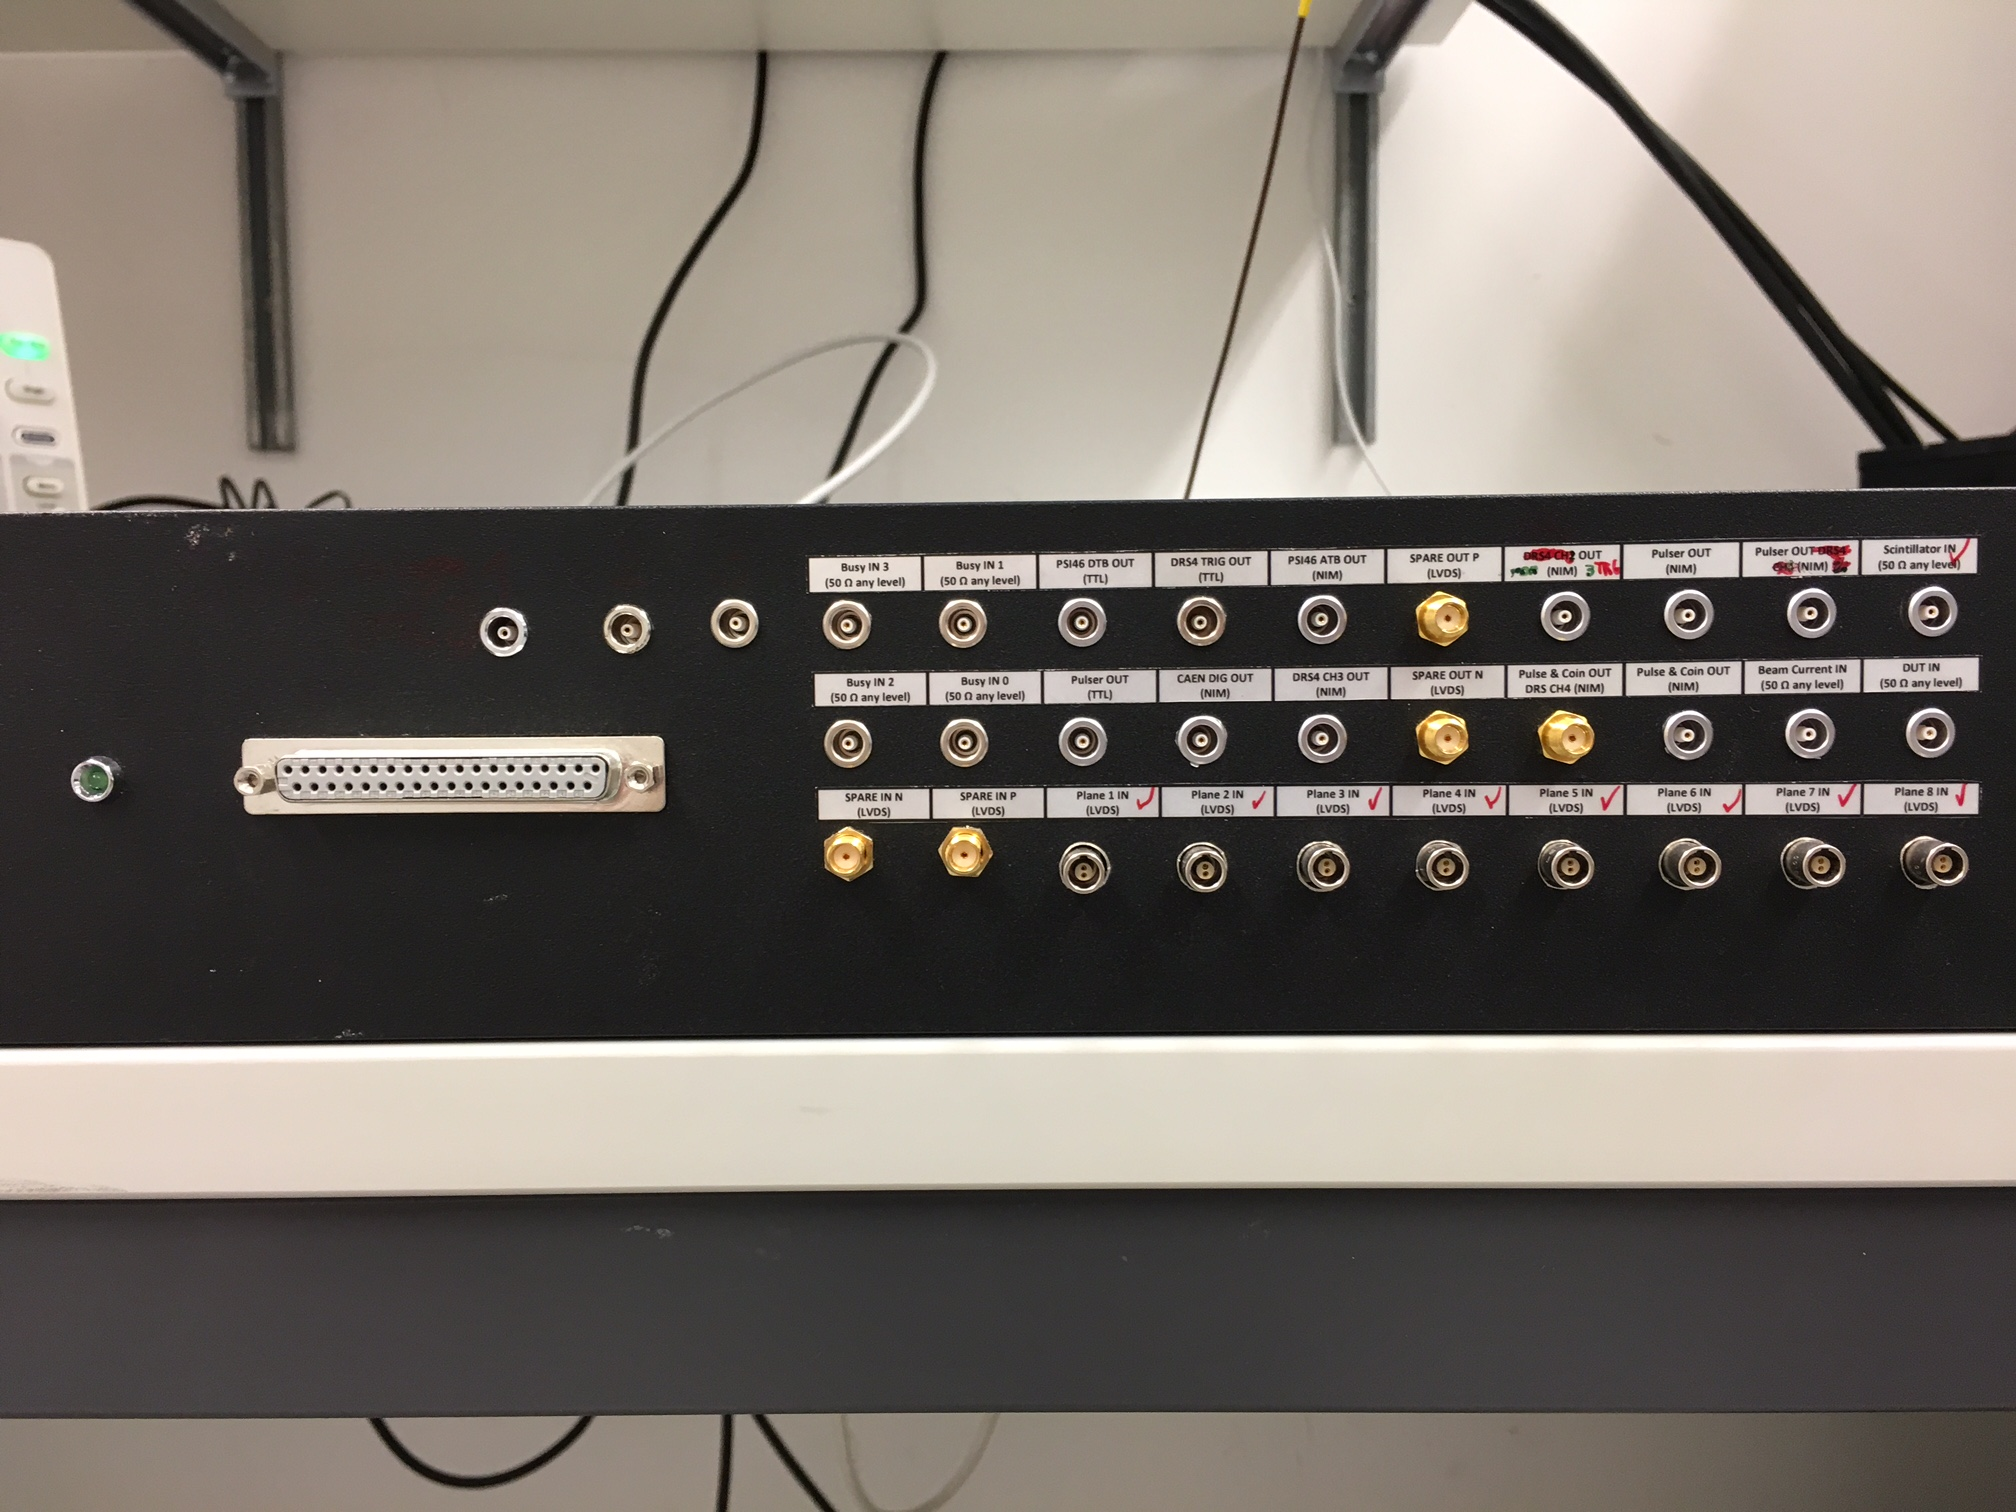
\includegraphics[width=.8\textwidth]{tu}
	\end{figure}
	\begin{itemize}
		\setlength{\itemsep}{\fill}
		\item handles (almost) all trigger logic of the setup with FPGA system
		\item provides scalers (counter) for the input triggers, pad signals and beam current
		\item sends calibration pulses as reference signal
		\item pre-scalers to guarantee stable pulser rates
		\item coincidence and handshake logic
	\end{itemize}
\end{frame}
% ============================ new frame ==========================================>
% END
% BEGIN ANALYSIS
\subsection{Analysis}
% ============================ FRAME 19 ==========================================>
\begin{frame}
	\frametitle{Waveforms}
	\vspace*{-20pt}
	\begin{center}
		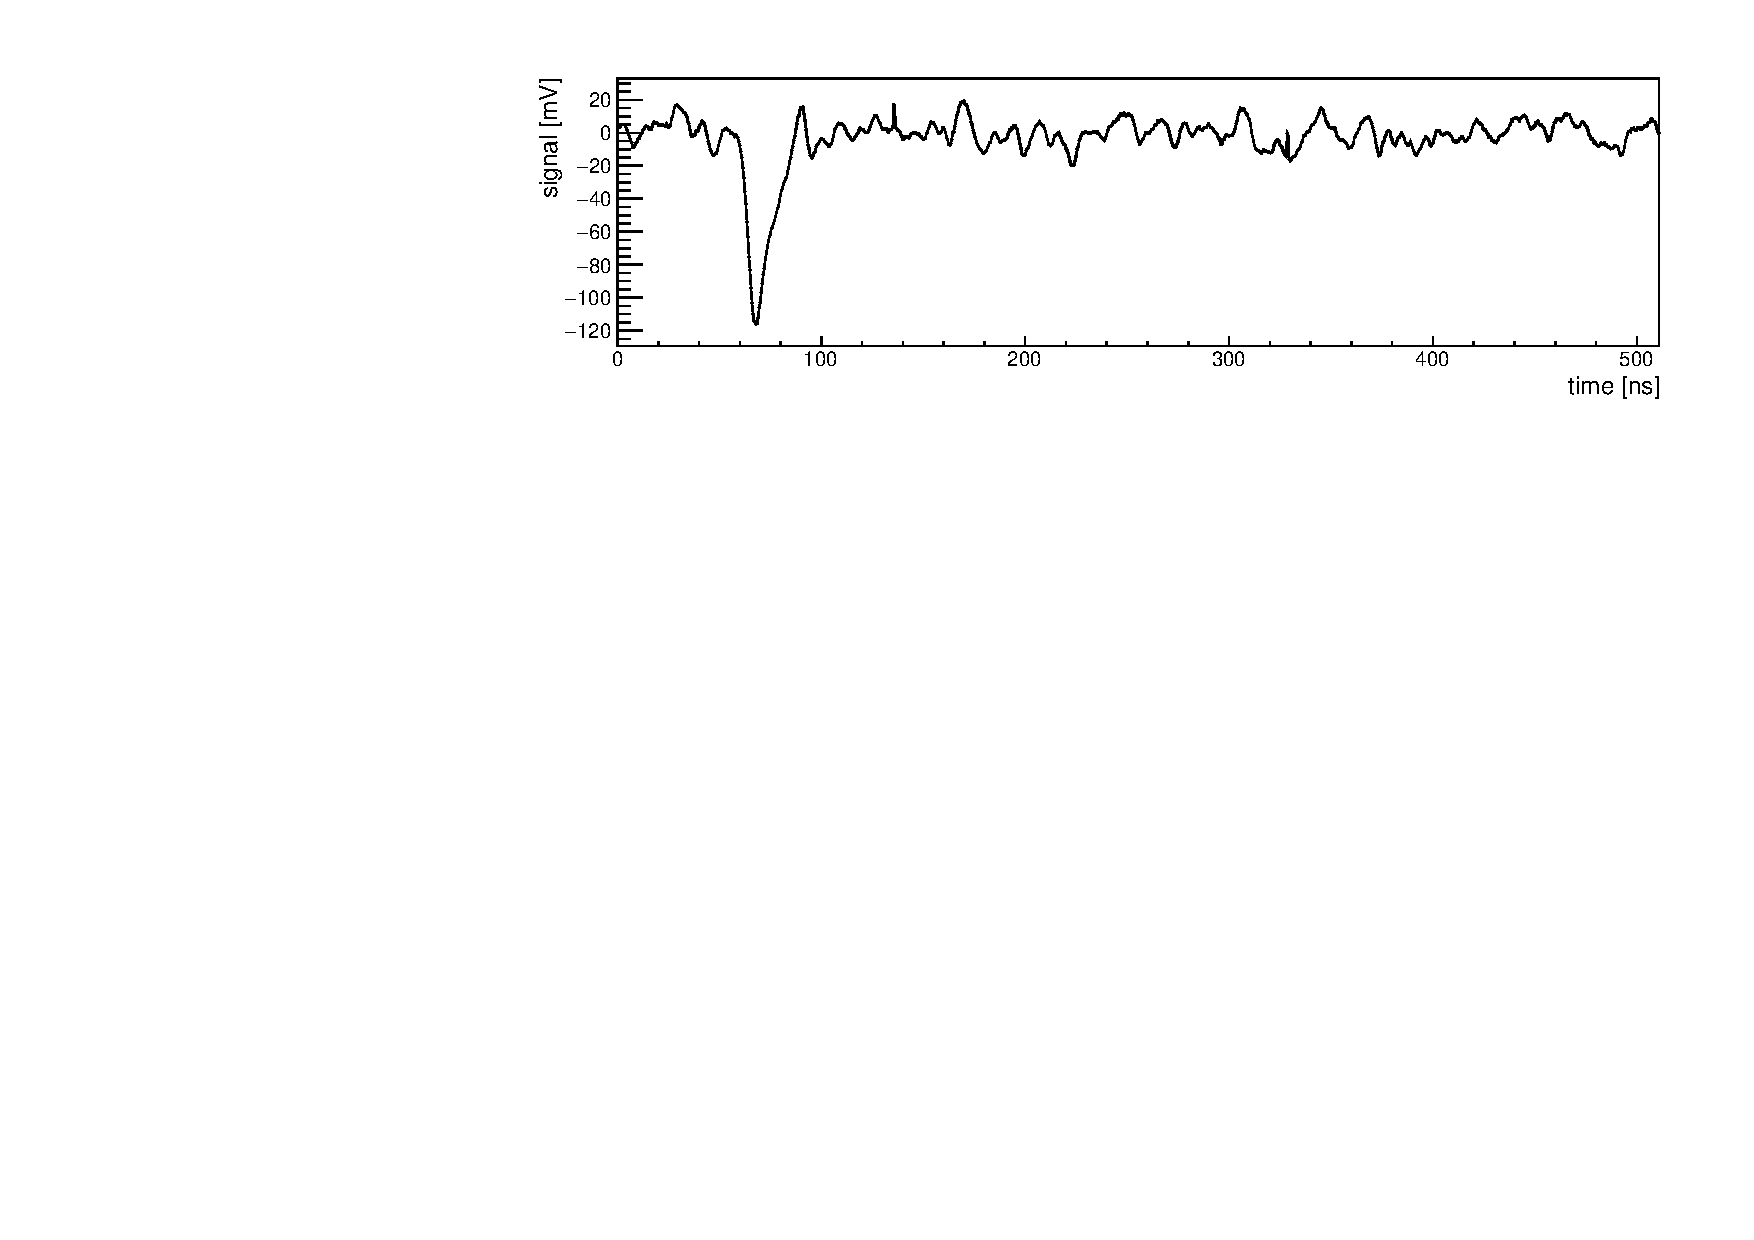
\includegraphics[angle=270, width=.7\textwidth]{SignalWaveform}\\
		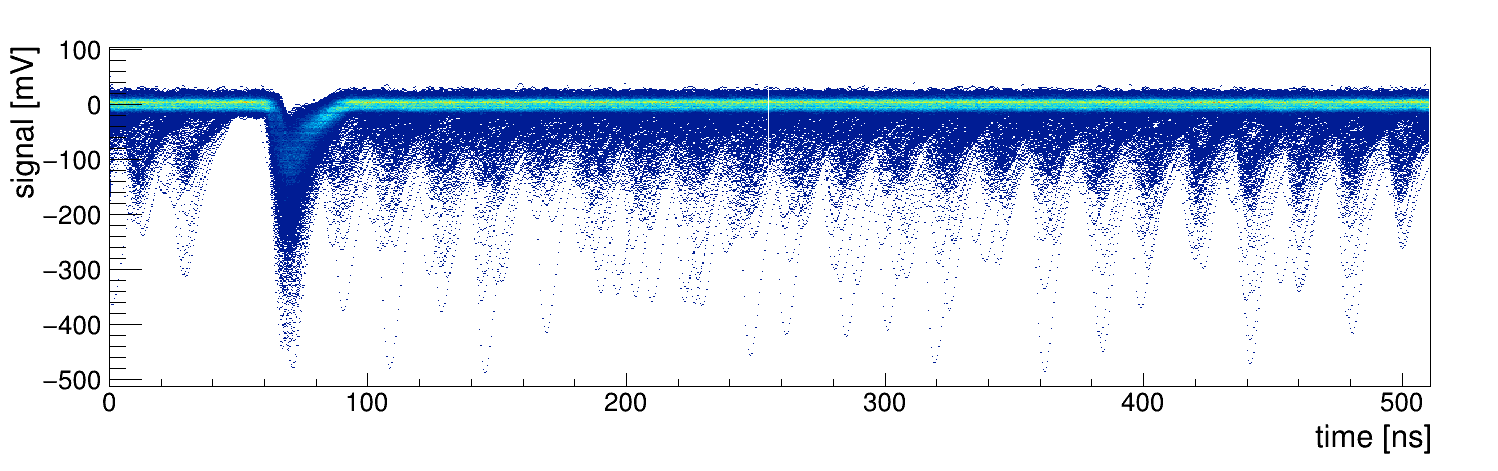
\includegraphics[width=.7\textwidth]{SignalWaveforms5000}
	\end{center}
	\begin{itemize}
		\item most frequented peak (\SI{\sim70}{ns}): triggered signal
		\item other peaks originate from other buckets ($\rightarrow$ resolve beam structure of \SI{\approx19.7}{ns})
		\item system does not allow signals in pre-signal bucket due to fastOR trigger deadtime
	\end{itemize}
\end{frame}
% ============================ FRAME 20 ==========================================>
\begin{frame}
	\frametitle{Pulse Height Calculation}
	\vspace*{-5pt}
	\begin{center}
		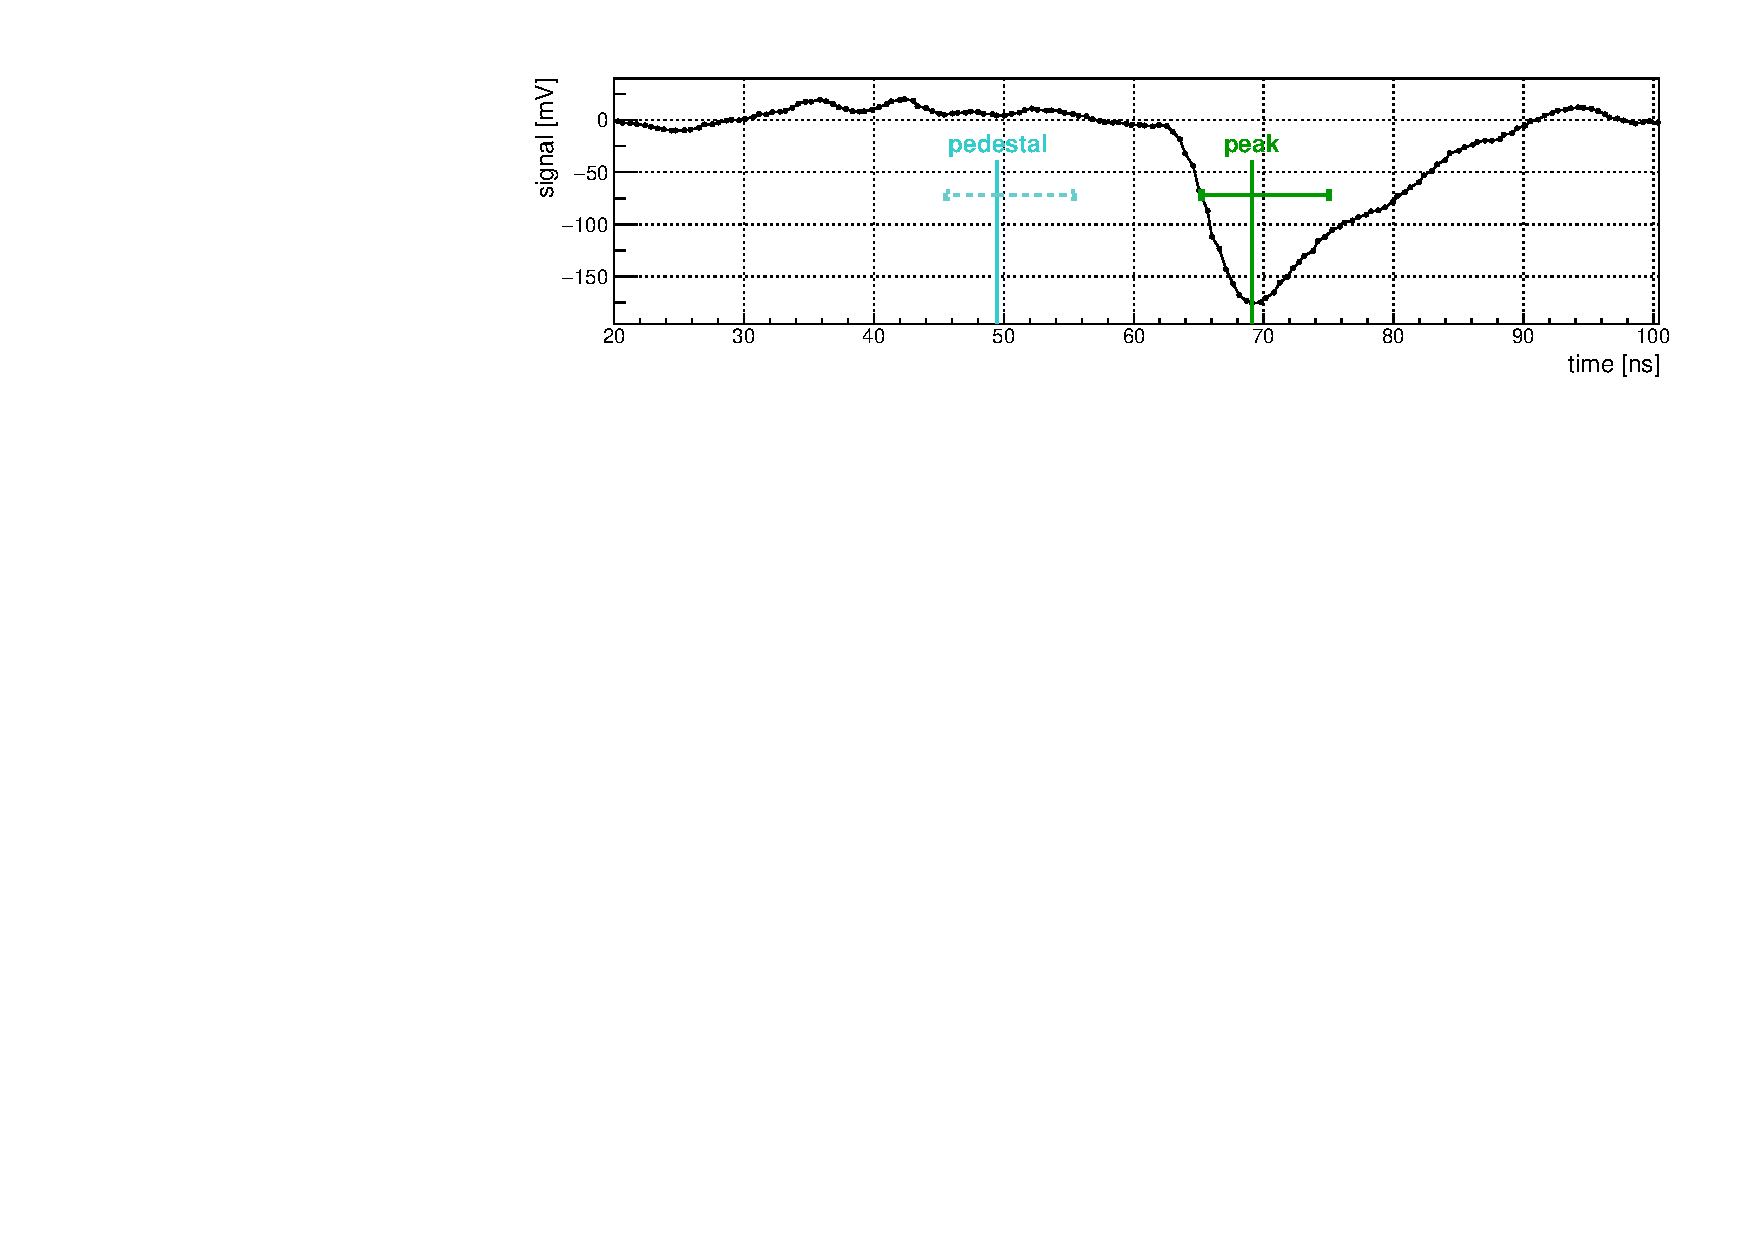
\includegraphics[angle=270, width=.8\textwidth]{intpeaks}\\
	\end{center}
	\vspace*{-5pt}
	\begin{itemize}
		\setlength{\itemsep}{\fill}
		\item finding the peak in the signal region
		\item integrating the signal in time fixed asymmetric integral around peak
		\item time averaging
		\item same procedure for pedestal (base line $\rightarrow$ noise)
		\item optimising the integral width by highest SNR (Integral / Pedestal Sigma)
		\item subtracting the pedestal from the signal integral on event-wise basis 
	\end{itemize}
\end{frame}
% ============================ FRAME 21 ==========================================>
\begin{frame}
	\frametitle{Event based cuts}
	\vspace*{-7pt}
	\begin{figure} 
		\begin{center}
			\begin{subfigure}{0.45\textwidth}  
				\centering 
				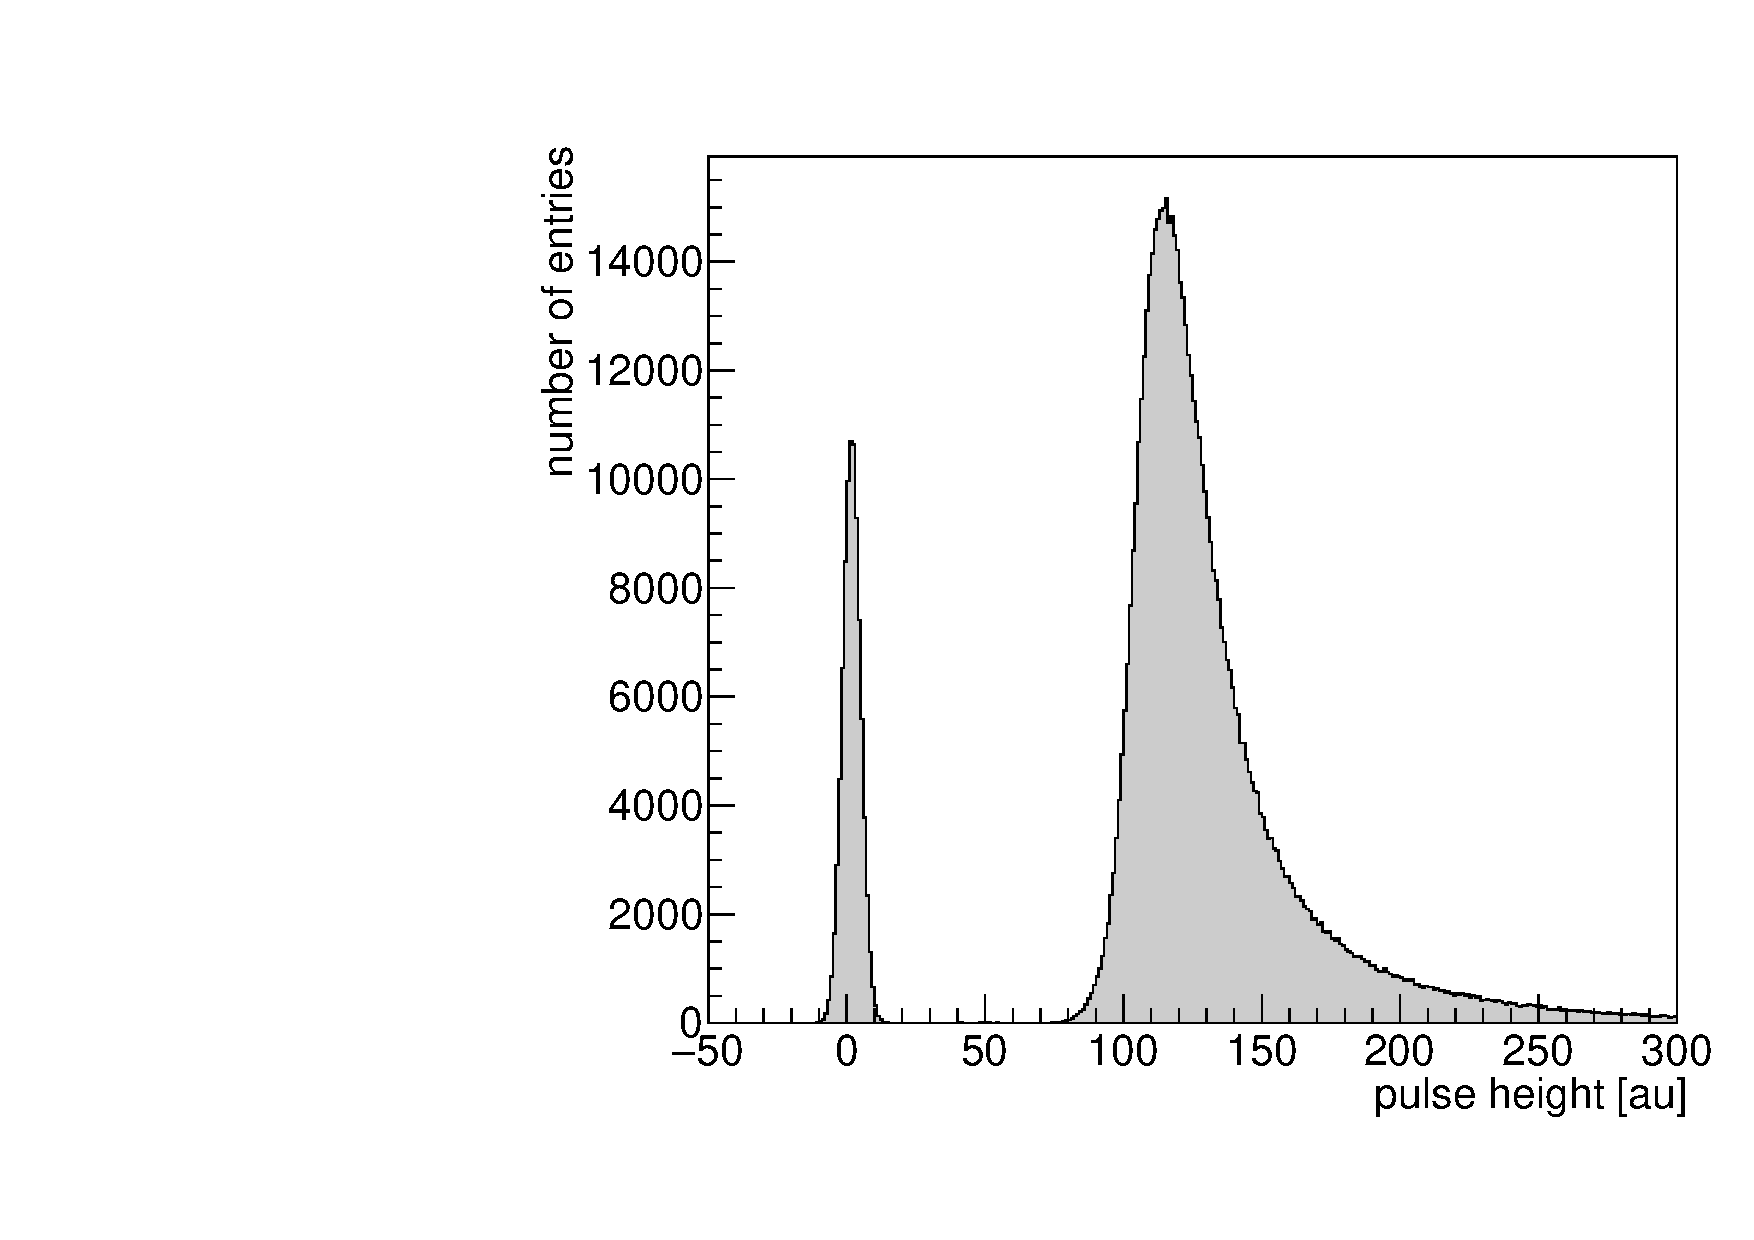
\includegraphics[angle=270, width=.85\textwidth]{DistoNoCuts}
				\caption{no cuts}
			\end{subfigure}
			\ra
			\begin{subfigure}{0.45\textwidth} 
				\centering 
				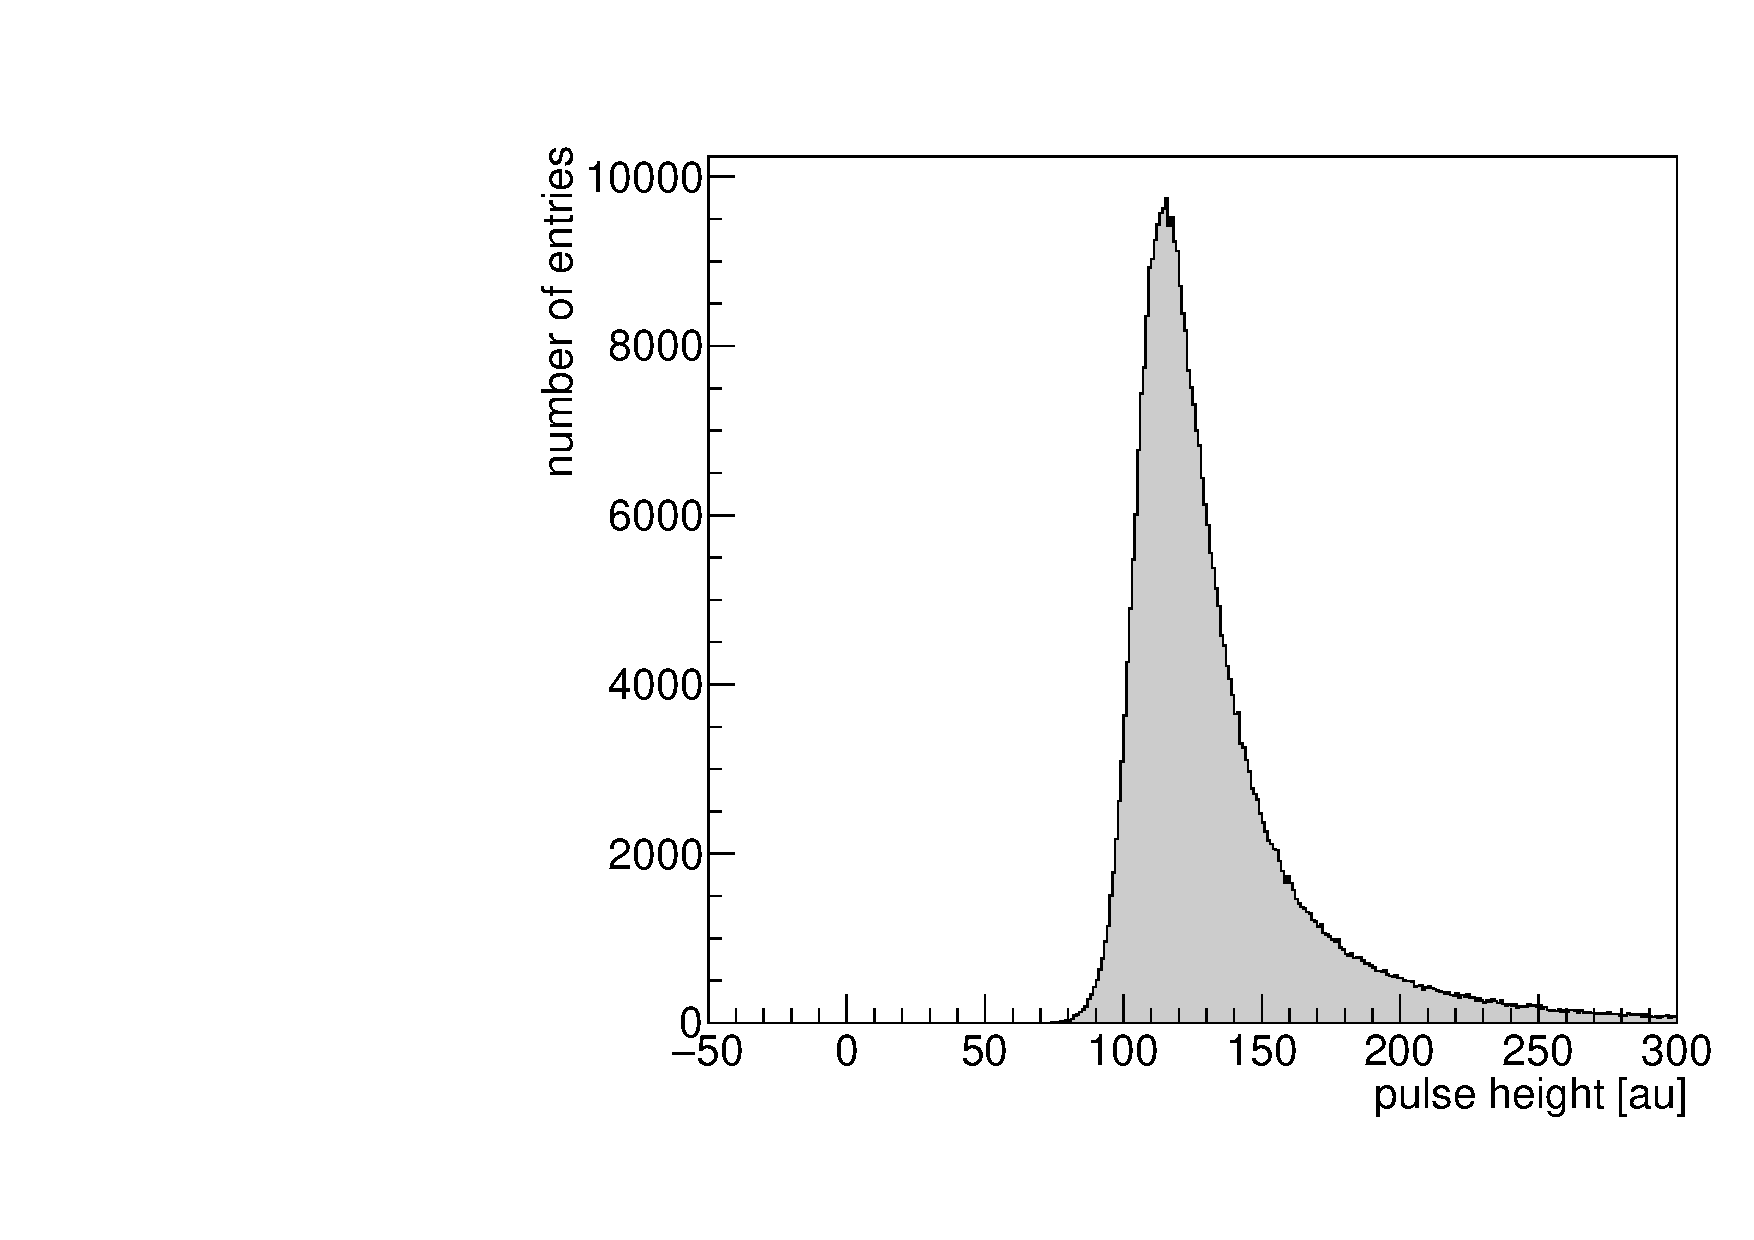
\includegraphics[angle=270, width=.85\textwidth]{DistoCuts}
				\caption{all cuts} 	
			\end{subfigure} 
		\end{center}
	\end{figure}
	\vspace*{-7pt}
	\begin{itemize}
		\setlength{\itemsep}{\fill}
		\item many undesirable events in the full data (no signal, pulser, multiple hits, $\hdots$)
		\item apply cuts to select only signal events (diamond hit by a single pion)
	\end{itemize}
\end{frame}
% ============================ FRAME 22 ==========================================>
\begin{frame}
	\frametitle{Cuts (1)}
	\begin{minipage}{8cm}
		\textbf{\underline{saturated:}}
		\begin{itemize}
			\setlength{\itemsep}{\fill}
			\item saturated waveforms
			\item most likely protons
		\end{itemize}
		\vspace*{1cm}
		\textbf{\underline{pulser:}}
		\begin{itemize}
			\setlength{\itemsep}{\fill}
			\item reference events with different timing
			\item no signal in signal region
		\end{itemize}
		\vspace*{1cm}
		\textbf{\underline{tracks:}}
		\begin{itemize}
			\setlength{\itemsep}{\fill}
			\item only take events with exactly one cluster in each tracking plane
		\end{itemize}
	\end{minipage}
	\begin{minipage}{4cm}
		\vspace*{-5pt}
		\begin{figure}
			\centering
			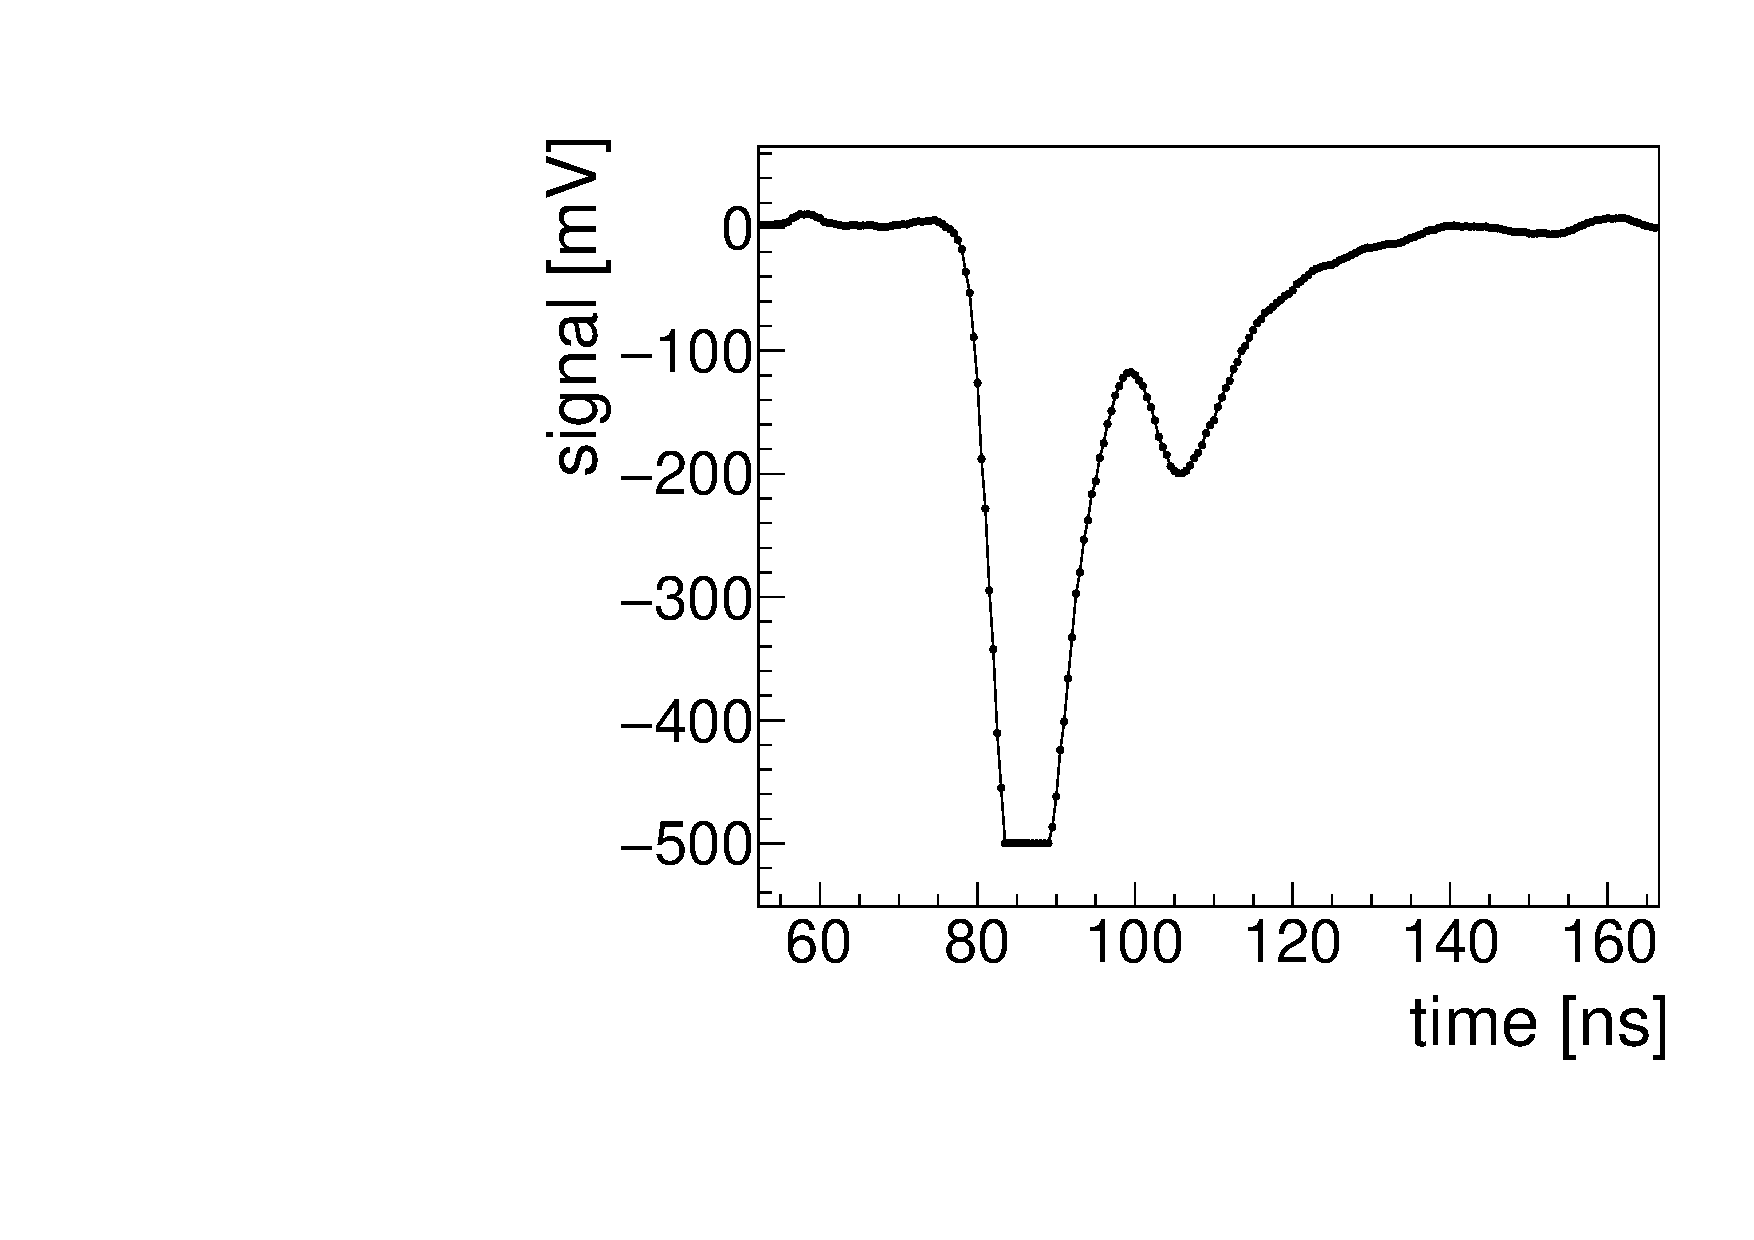
\includegraphics[angle=270, width=3.5cm]{Sat}
			\vspace*{-8pt}
			\caption{saturated waveform}
		\end{figure}
		\vspace*{-25pt}
		\begin{figure}
			\centering
			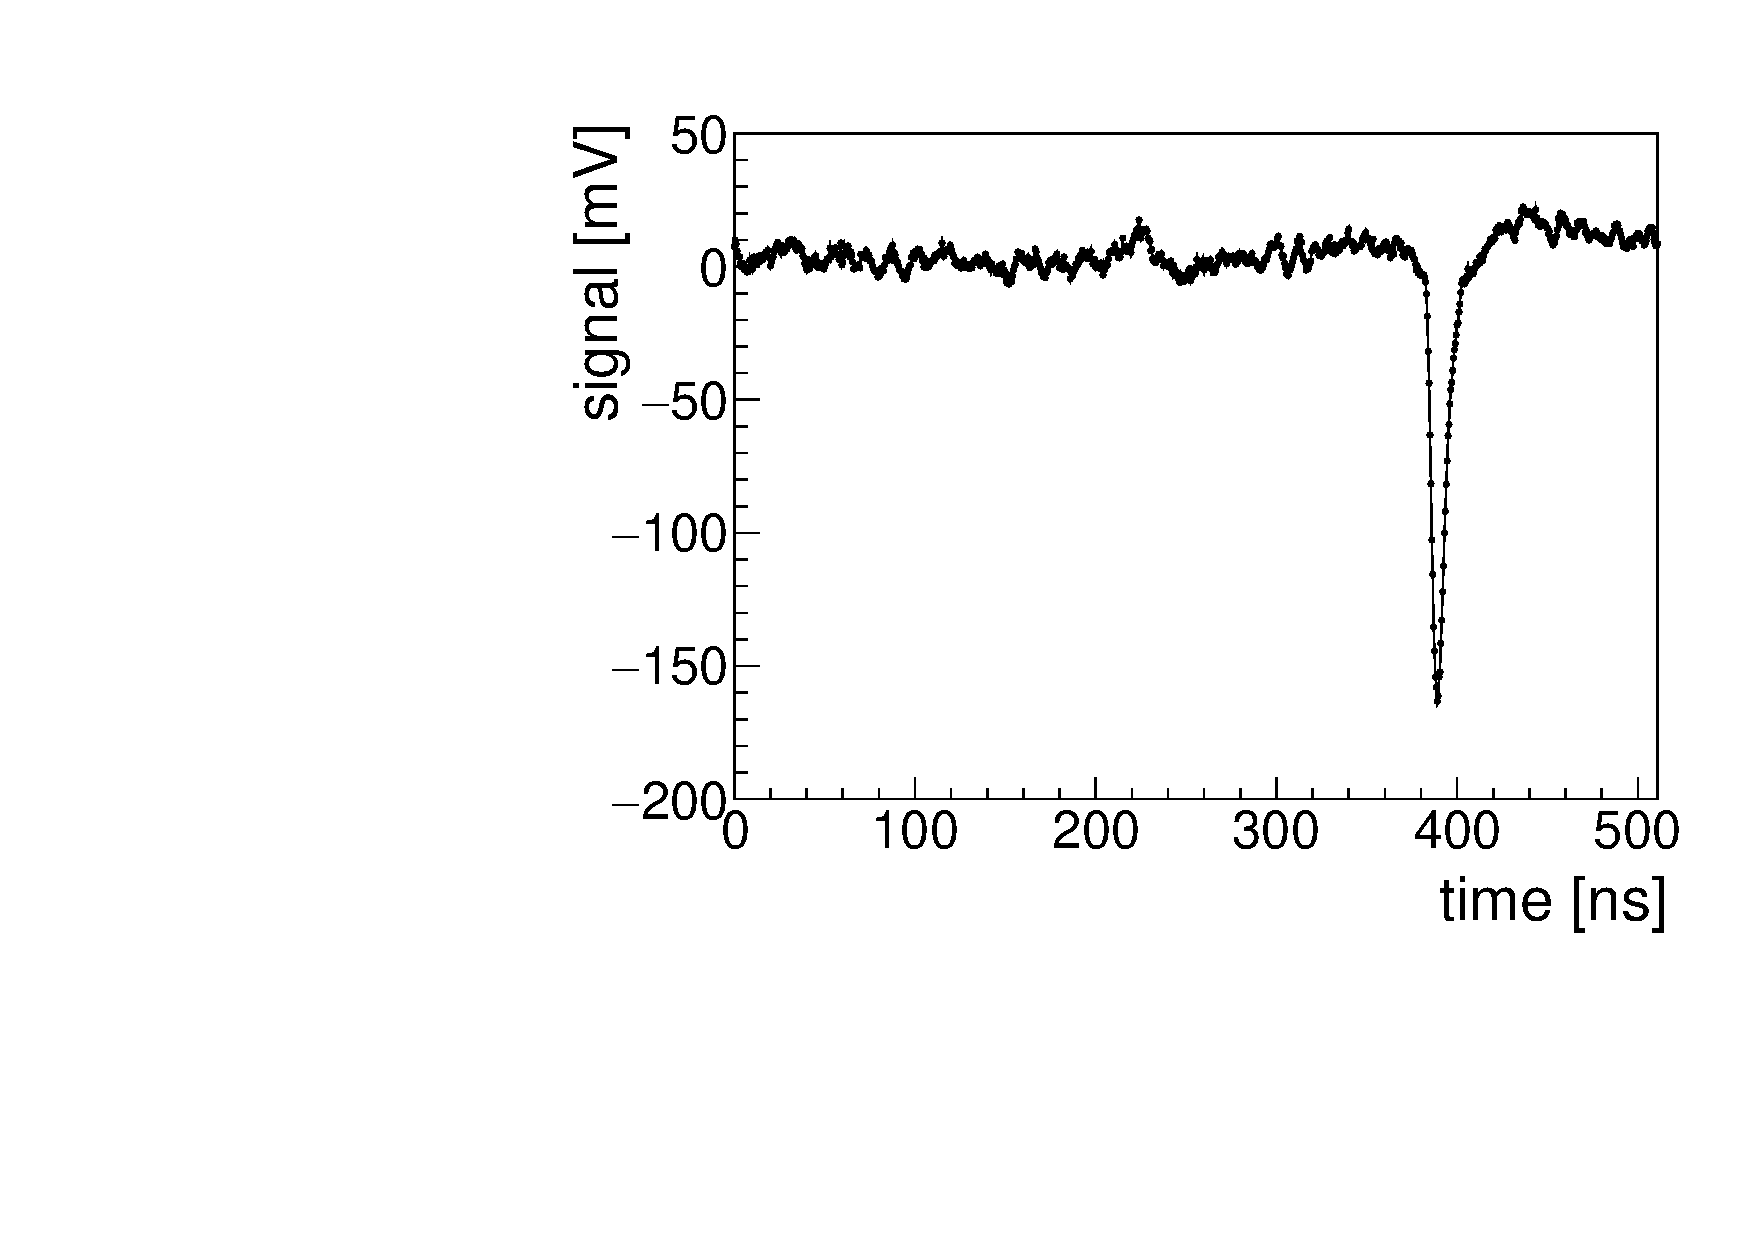
\includegraphics[angle=270, width=3.5cm]{Pul}
			\vspace*{-8pt}
			\caption{pulser waveform}
		\end{figure}
	\end{minipage}
\end{frame}
% ============================ FRAME 23 ==========================================>
\begin{frame}
	\frametitle{Cuts (2)}
	\begin{minipage}{8cm}
		\textbf{\underline{timing:}}
		\begin{itemize}
			\setlength{\itemsep}{\fill}
			\item signal peak timing follows Gaussian distribution
			\item discard events with wrong timing (more than \SI{3}{\upsigma})
			\begin{itemize}
				\item overlay from waveforms of different buckets
				\item other particles (electrons, muons)
			\end{itemize}
		\end{itemize}
		\vspace*{1cm}
		\textbf{\underline{bucket:}}
		\begin{itemize}
			\setlength{\itemsep}{\fill}
			\item two particles in consecutive buckets 
			\item first one hits the scintillator but not the diamond
			\item wrong trigger timing (\SI[retain-explicit-plus]{20}{ns})
			\item no signal in signal region
		\end{itemize}
	\end{minipage}
	\begin{minipage}{4cm}
		\vspace*{-2pt}
		\begin{figure}
			\centering
			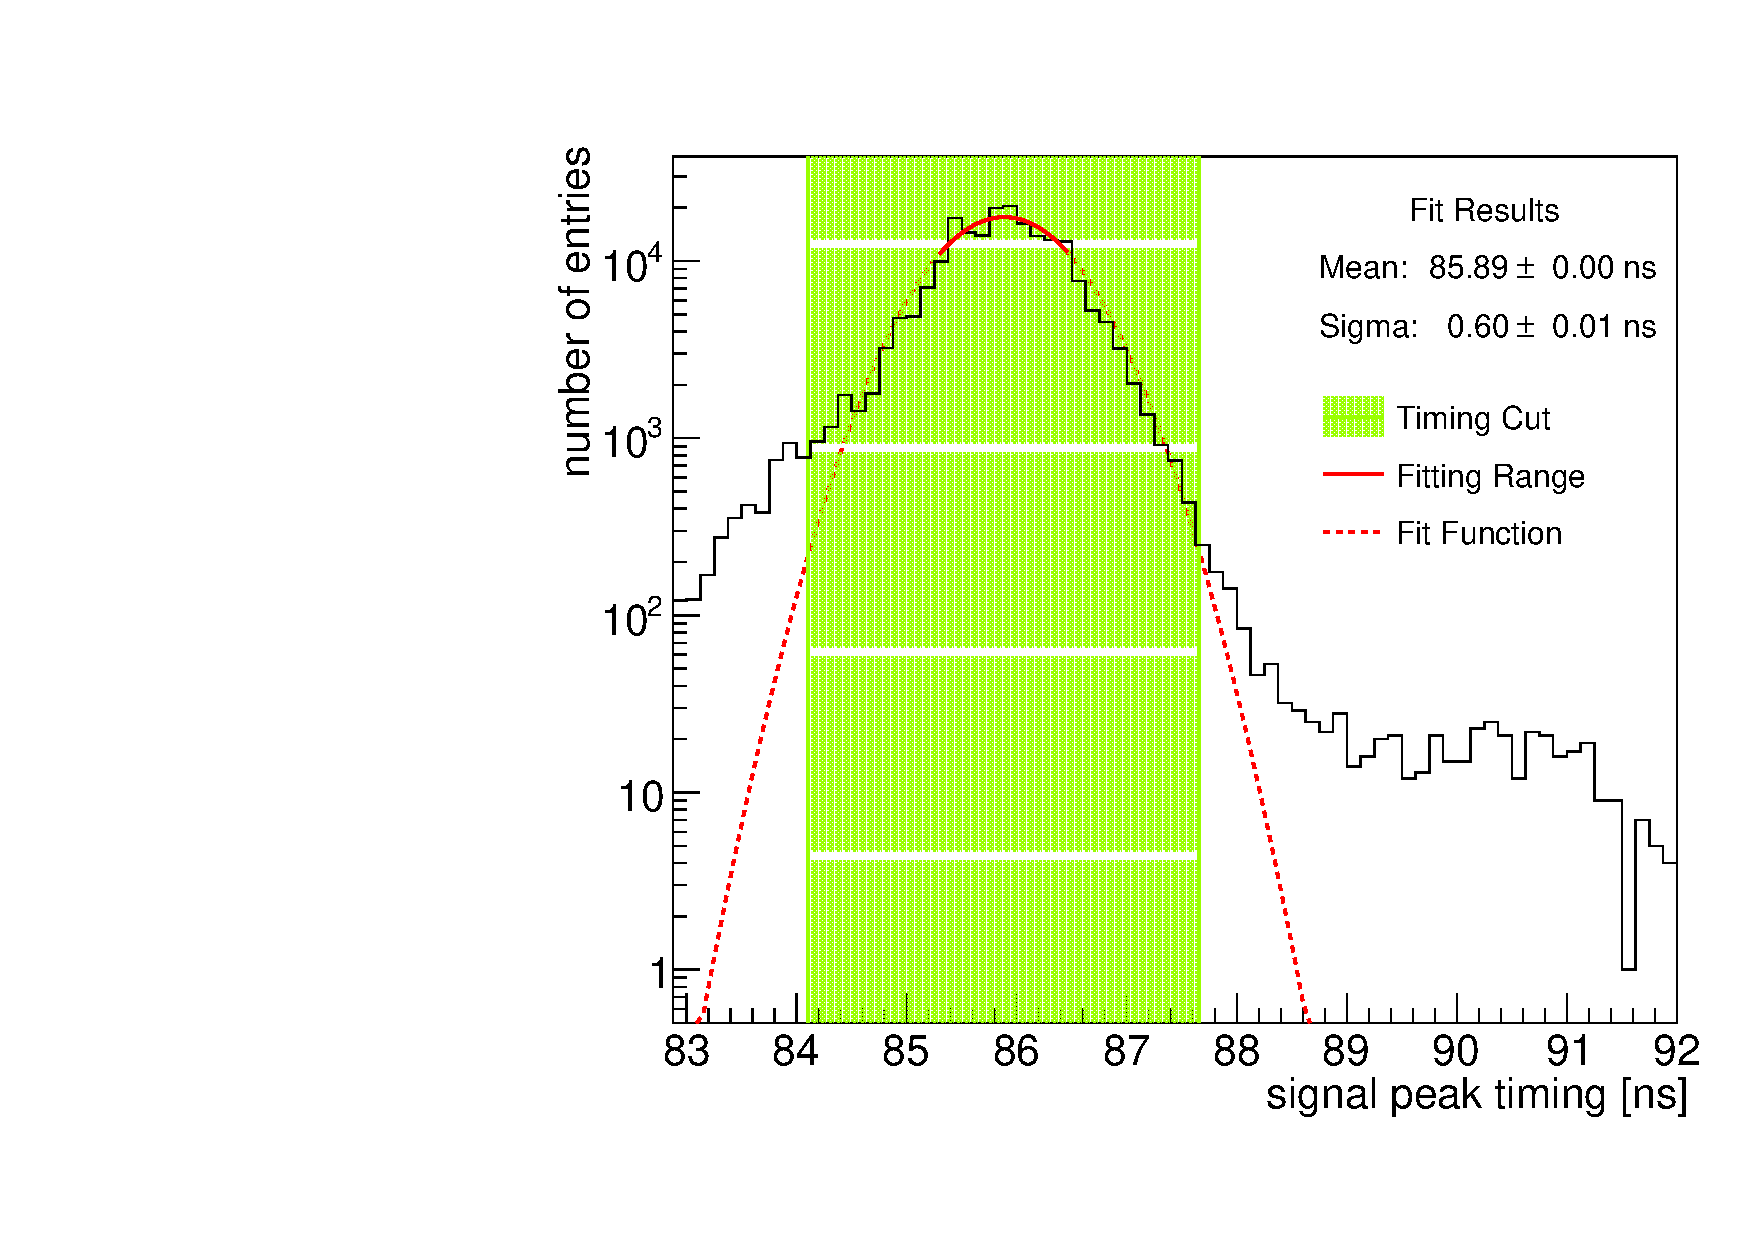
\includegraphics[angle=270, width=3.2cm]{Timing}
			\vspace*{-8pt}
			\caption{signal peak timing}
		\end{figure}
		\vspace*{-25pt}
		\begin{figure}
			\centering
			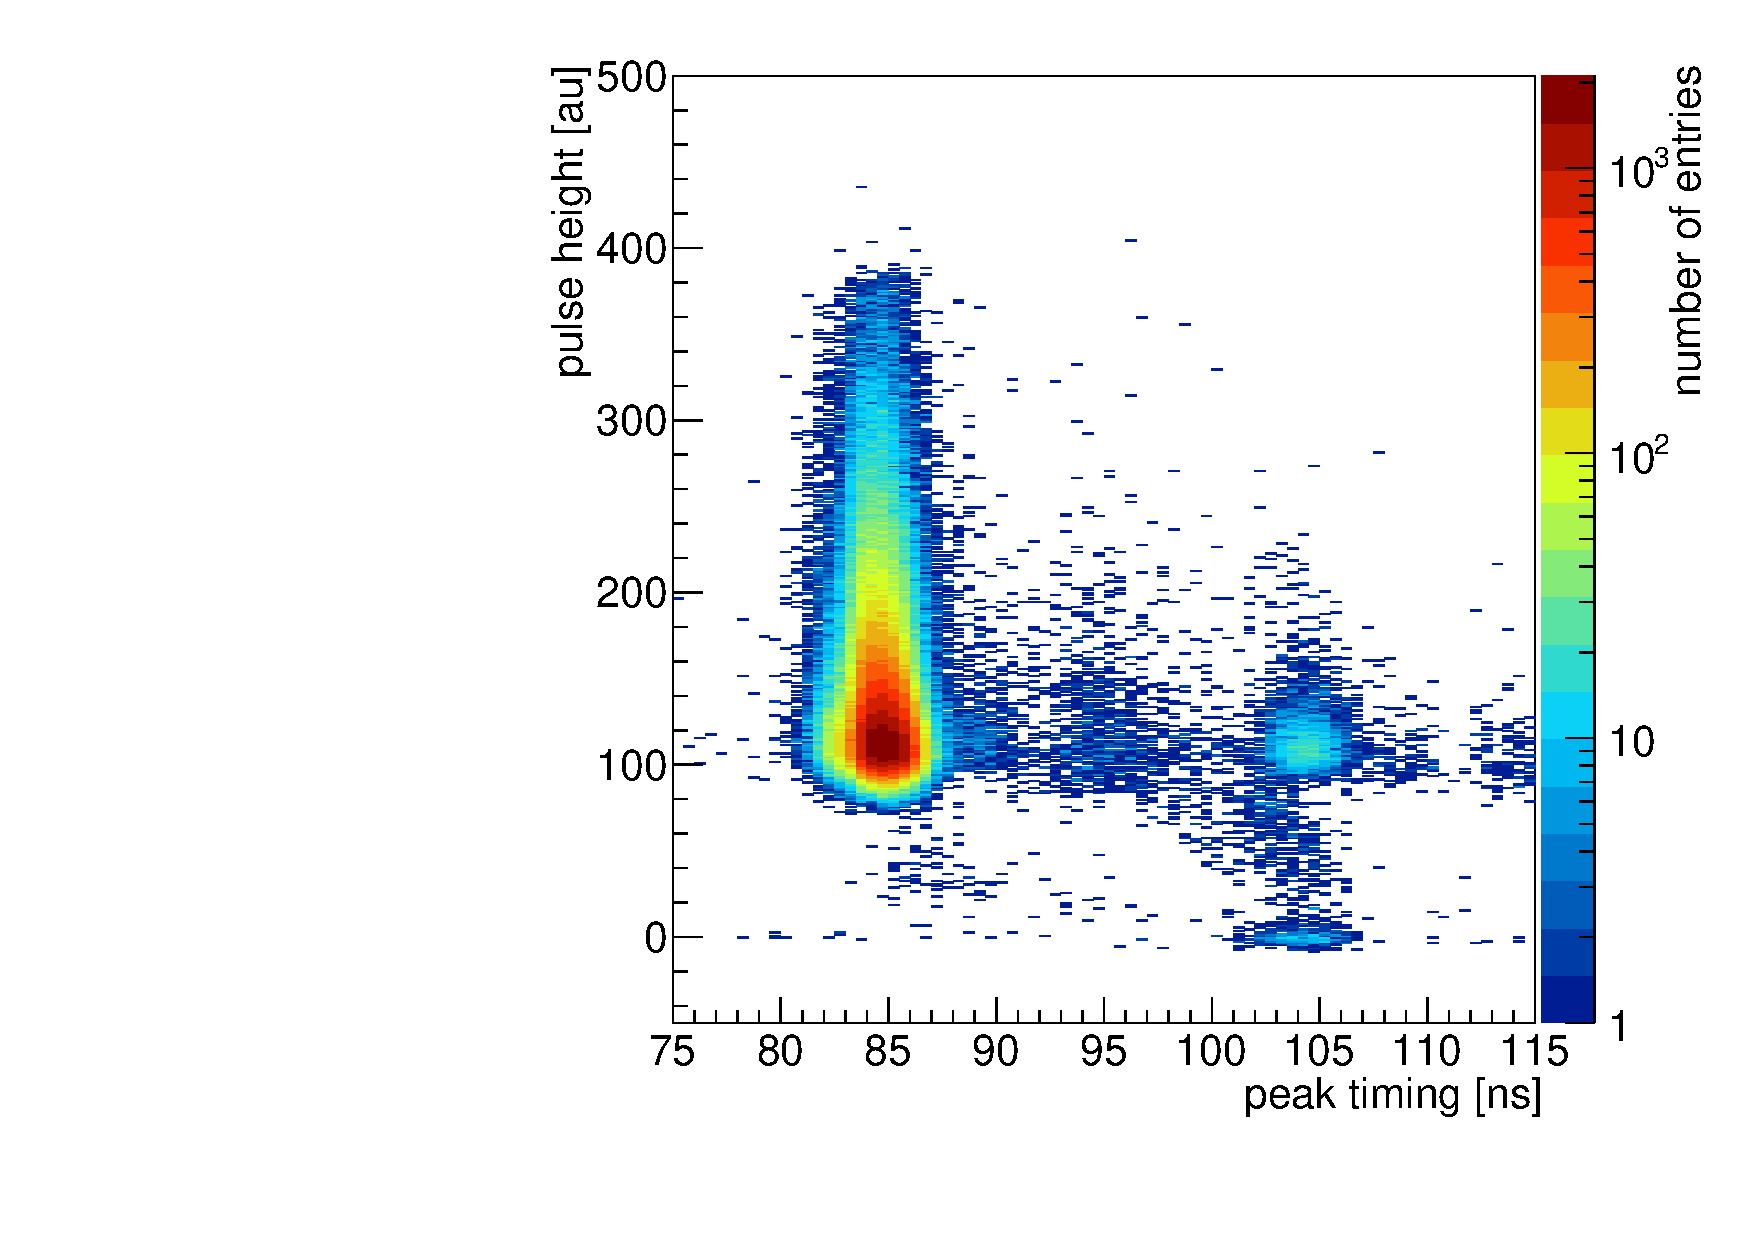
\includegraphics[angle=270, width=3.2cm]{Bucket}
			\vspace*{-8pt}
			\caption{bucket pedestal}
		\end{figure}
	\end{minipage}
\end{frame}
% ============================ FRAME 24 ==========================================>
\begin{frame}
	\frametitle{Cuts (3)}
	\begin{minipage}{8cm}
		\textbf{\underline{fiducial:}}
		\begin{itemize}
			\setlength{\itemsep}{\fill}
			\item only select uniform physical center area of the diamond 
			\item exclude edges and guard ring 
		\end{itemize}
		\vspace*{1cm}
		\textbf{\underline{other:}}
		\begin{itemize}
			\setlength{\itemsep}{\fill}
			\item $\upchi^{2}$ in $x$ and $y$ of the track fit
			\item track angle in $x$ and $y$
			\item event range
			\item beam interruptions
			\item pedestal sigma
		\end{itemize}
	\end{minipage}
	\begin{minipage}{4cm}
		\vspace*{-2pt}
		\begin{figure}
			\centering
			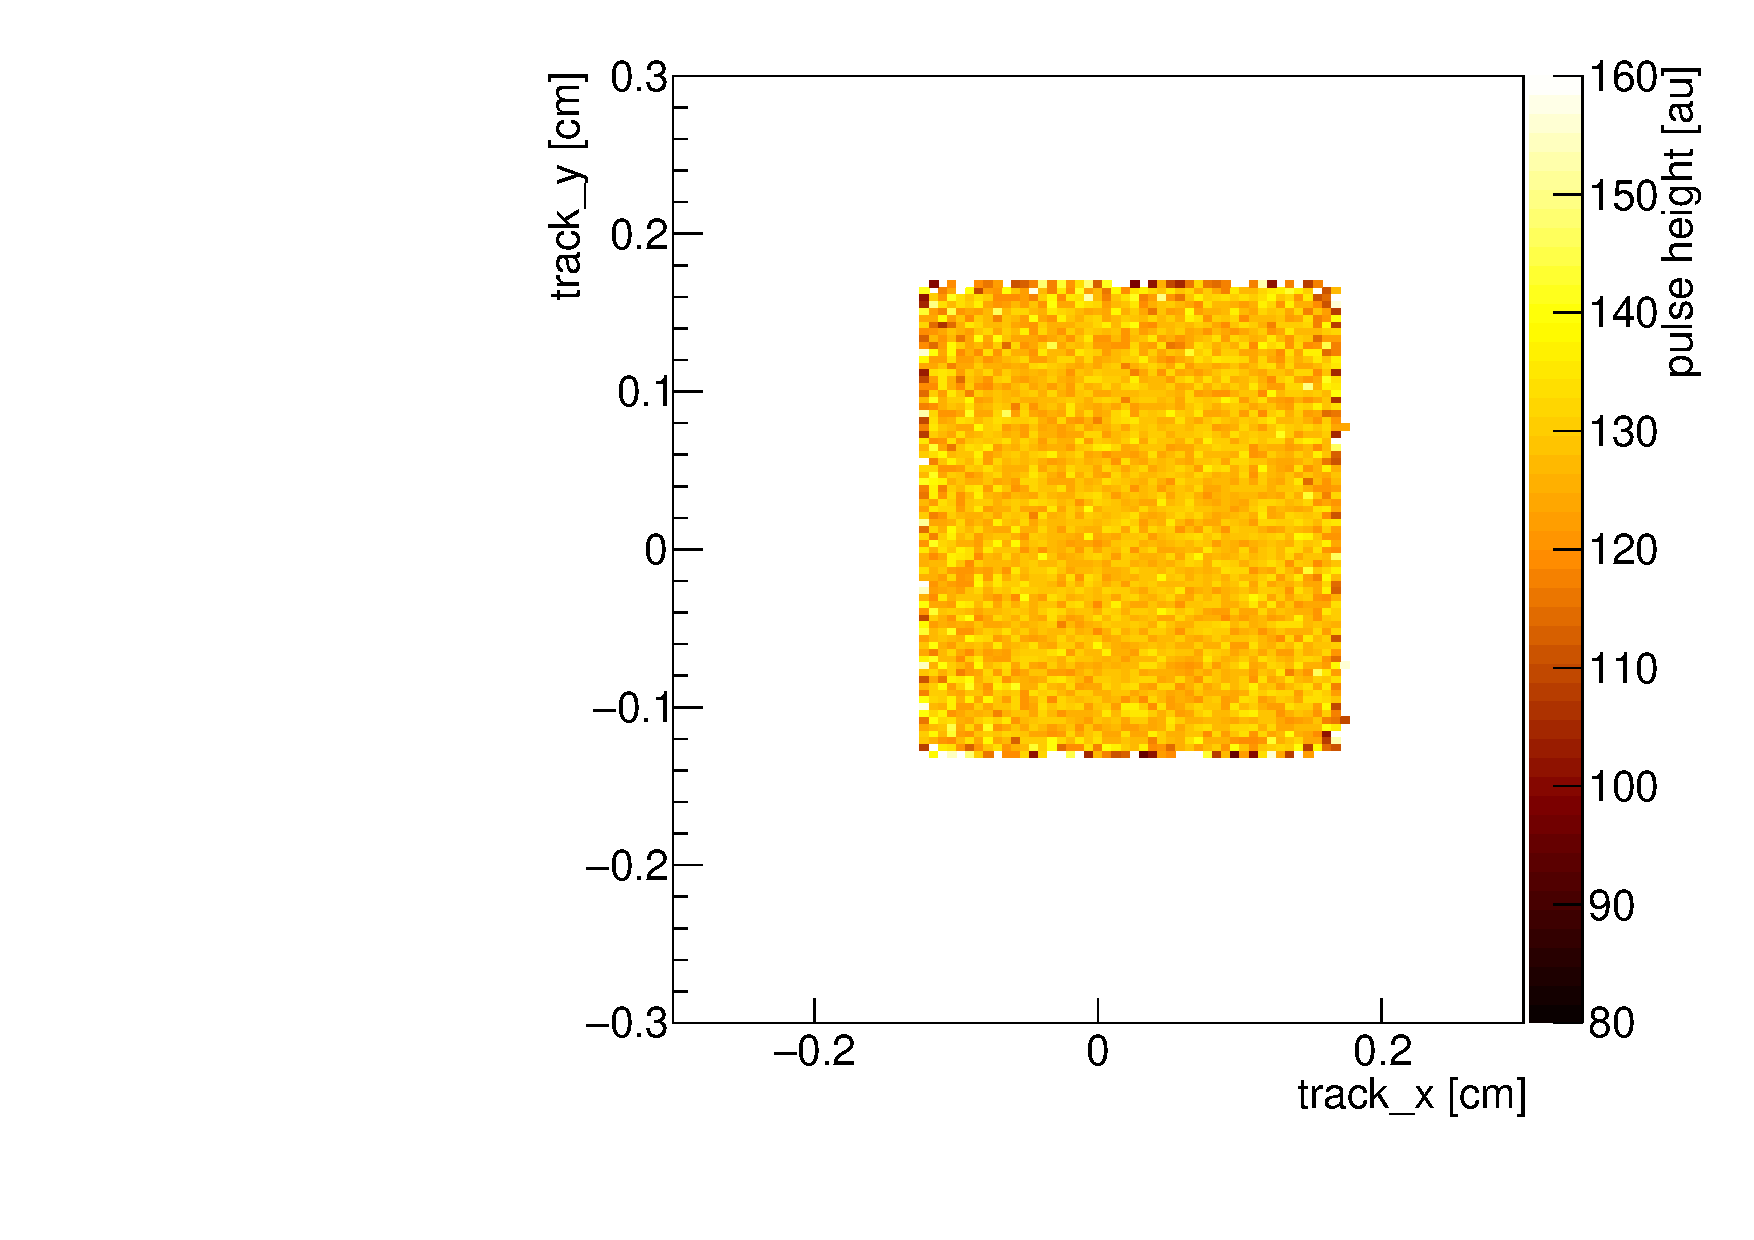
\includegraphics[angle=270, width=3.2cm]{FidNo}
			\vspace*{-8pt}
			\caption{signal map}
		\end{figure}
		\vspace*{-25pt}
		\begin{figure}
			\centering
			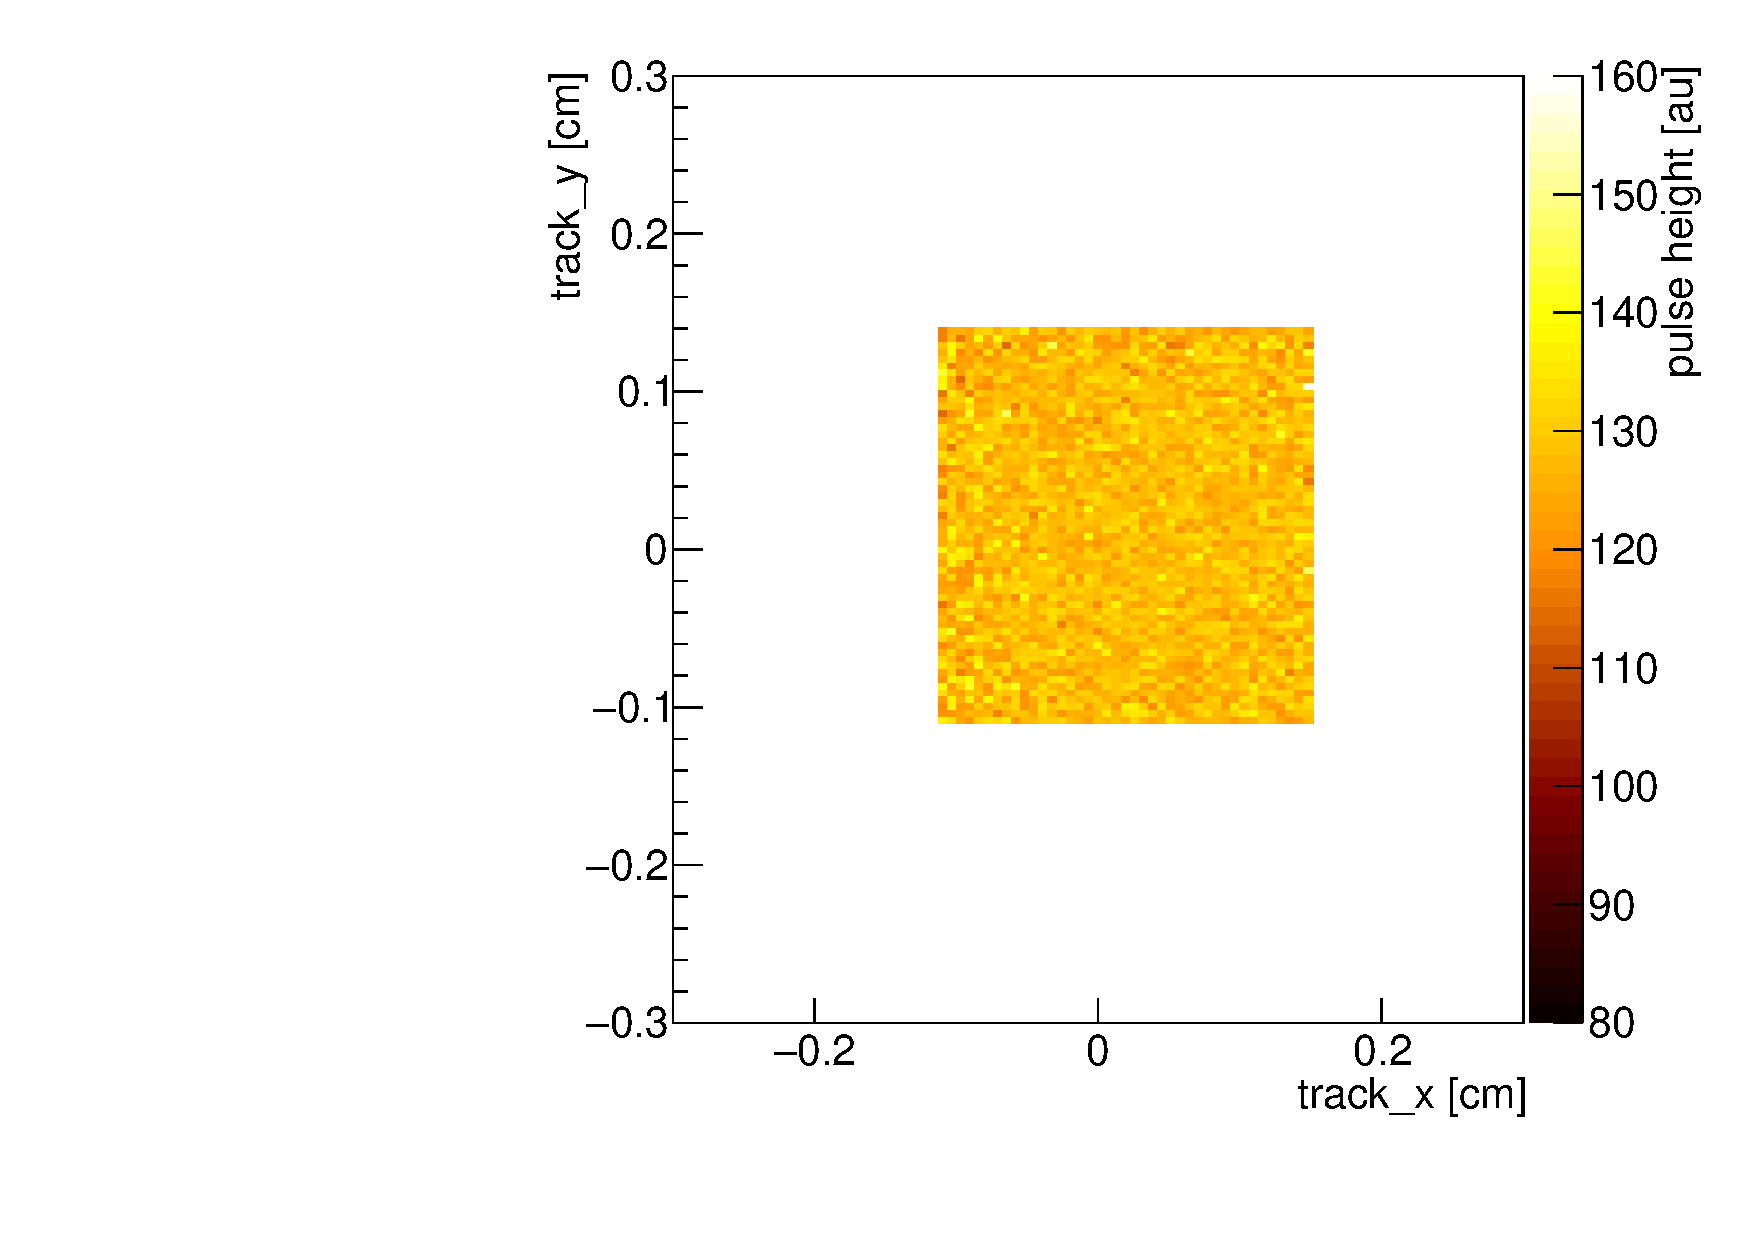
\includegraphics[angle=270, width=3.2cm]{Fid}
			\vspace*{-8pt}
			\caption{with fiducial cut}
		\end{figure}
	\end{minipage}
\end{frame}
% ============================ FRAME 25 ==========================================>
\begin{frame}
	\vspace*{-5pt}
	\begin{figure} 
		\begin{center}
			\begin{subfigure}{0.45\textwidth}  
				\centering 
				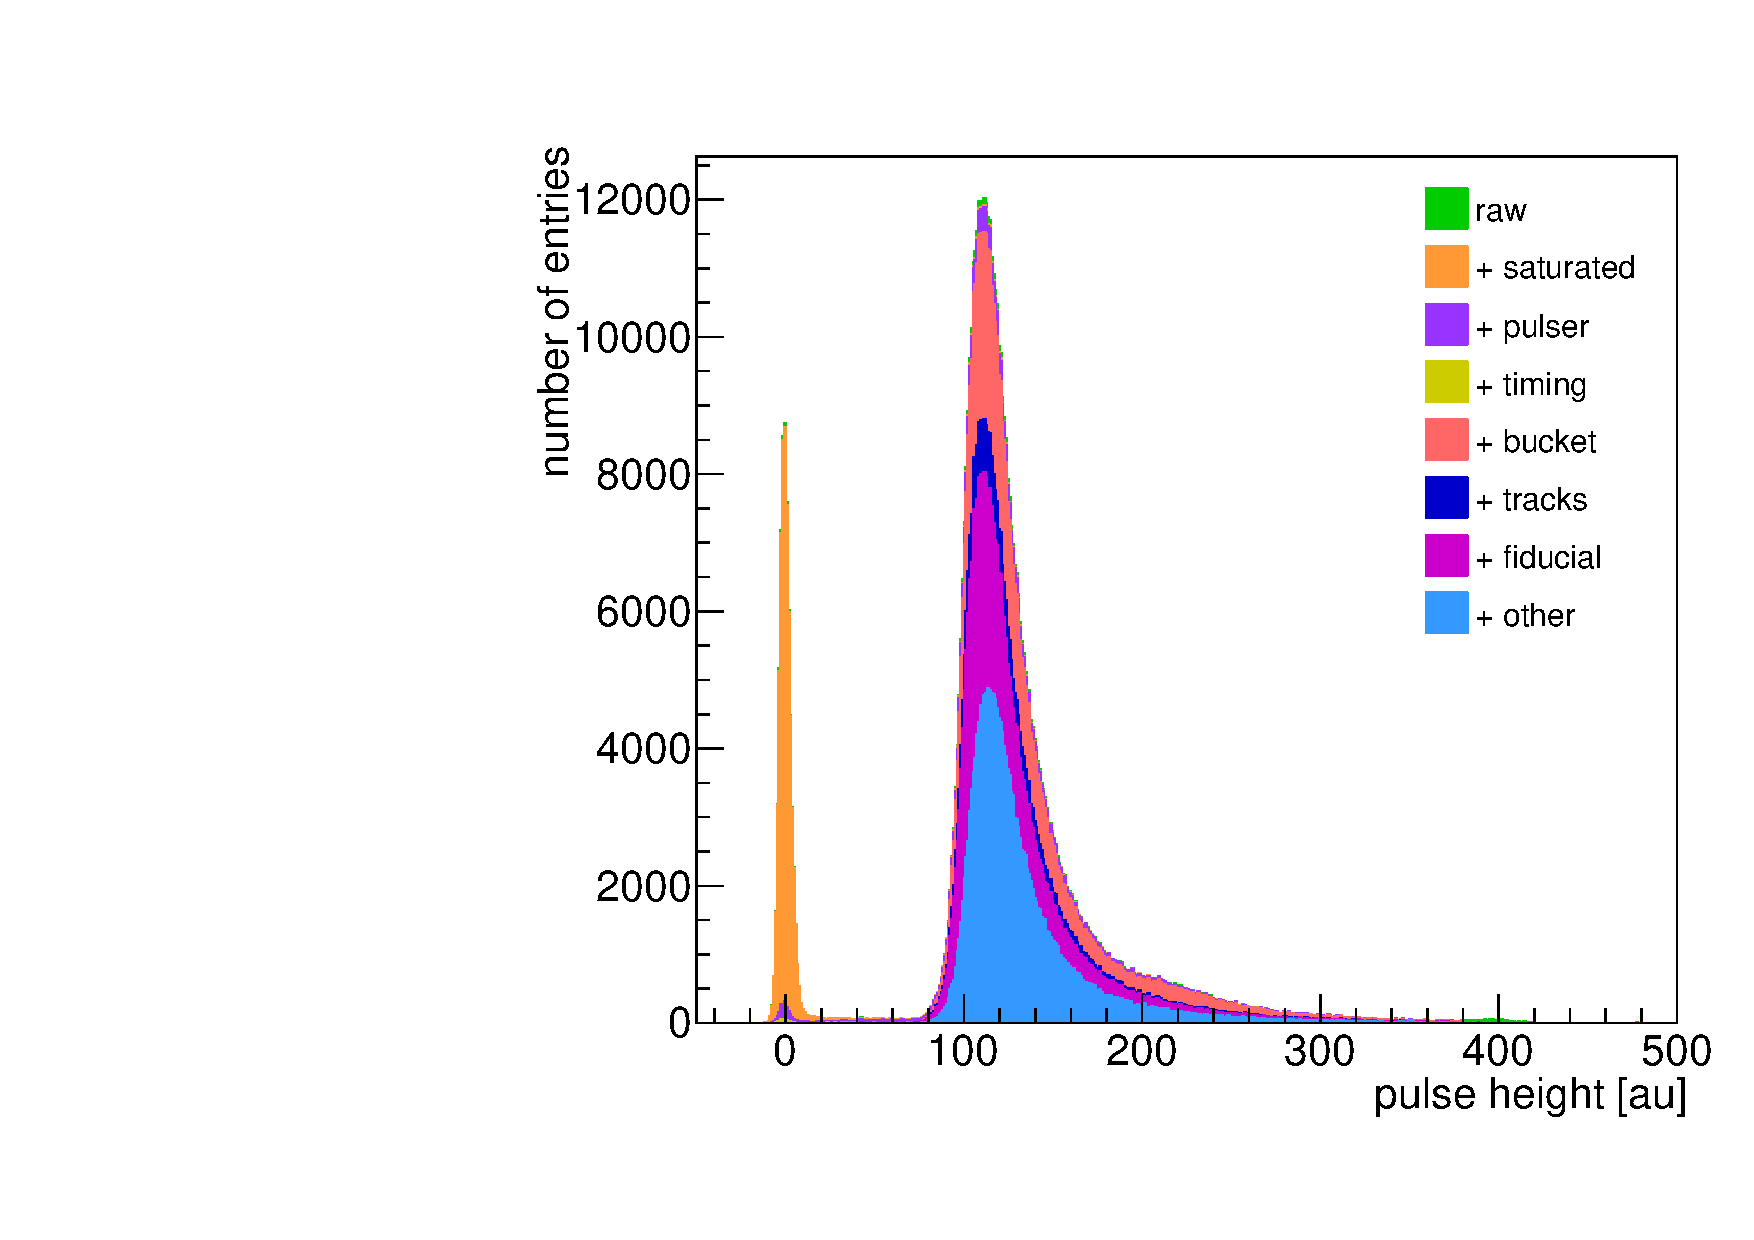
\includegraphics[angle=270, width=.85\textwidth]{Cuts}
% 				\caption{no cuts}
			\end{subfigure}
			\begin{subfigure}{0.45\textwidth} 
				\centering 
				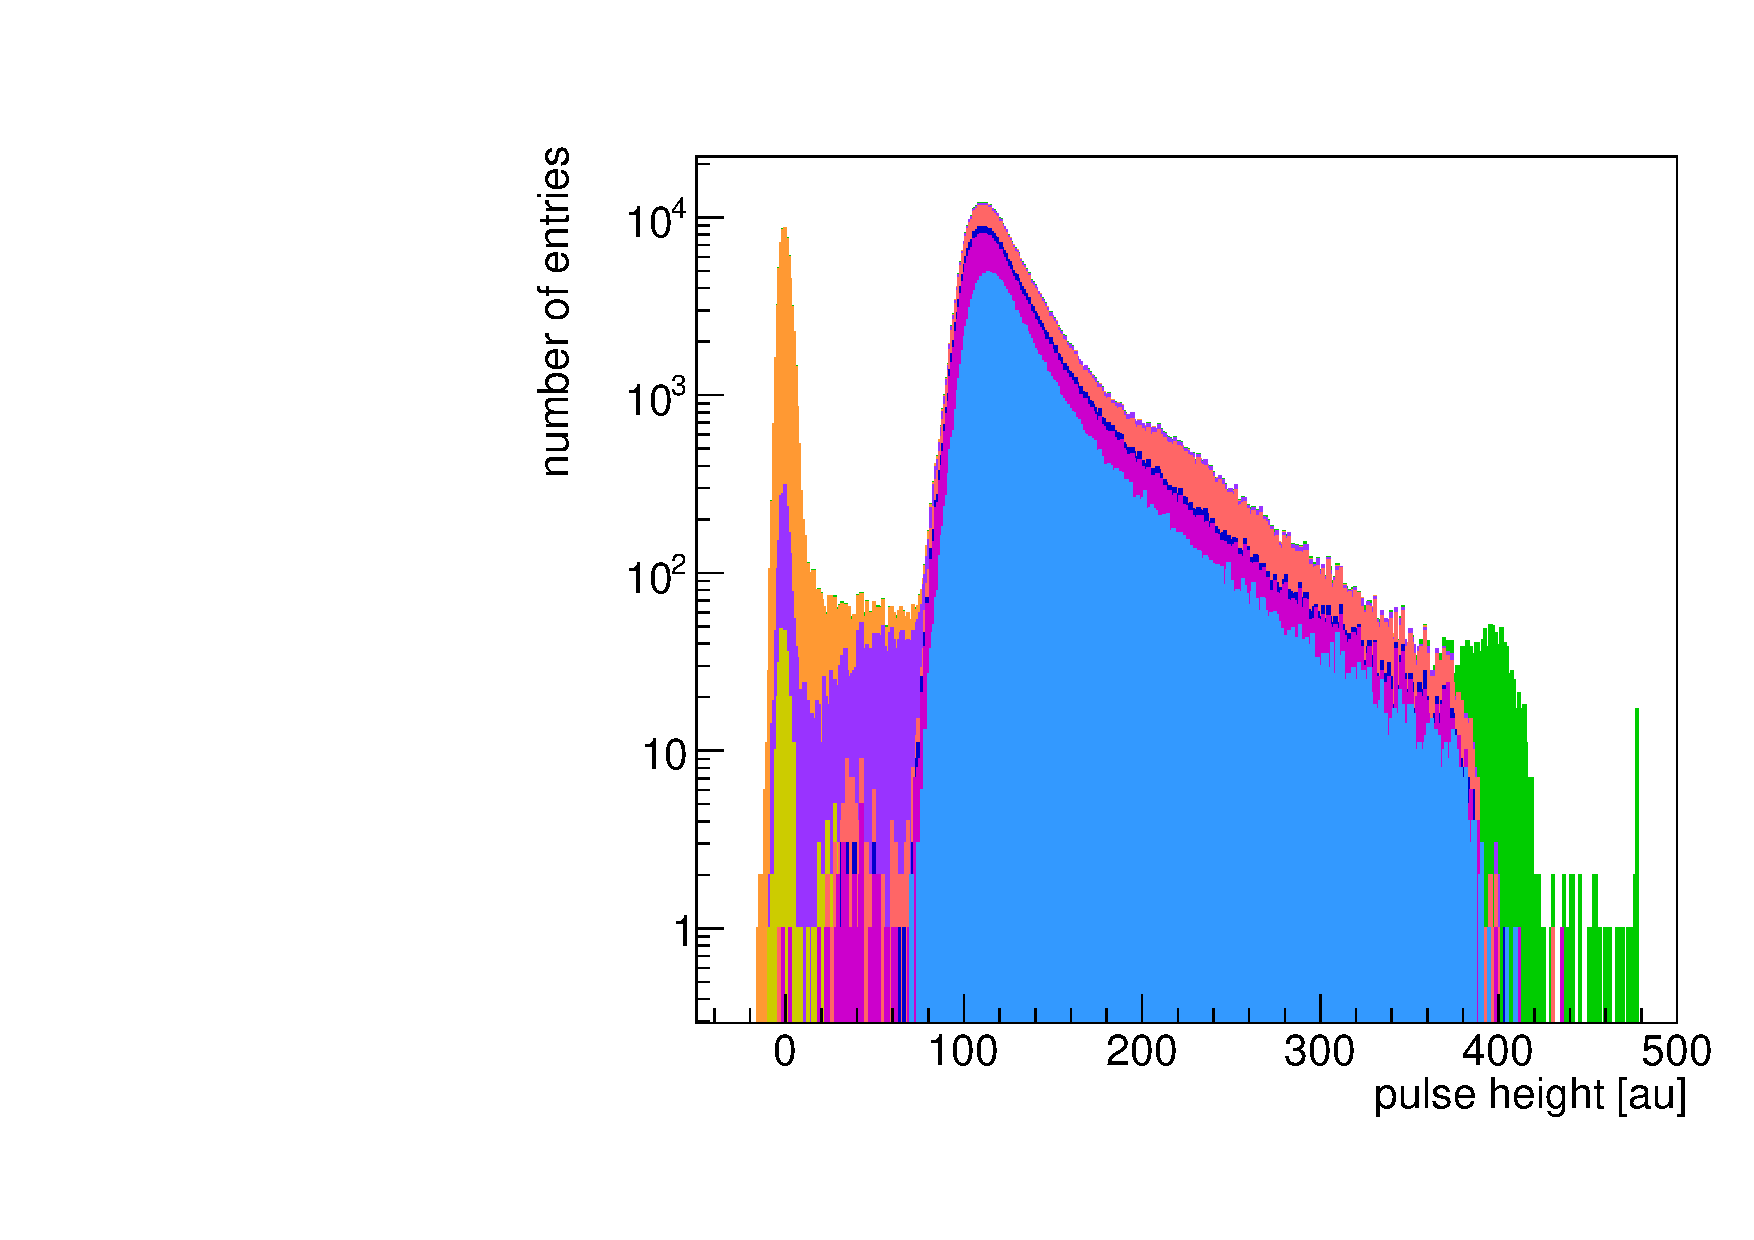
\includegraphics[angle=270, width=.85\textwidth]{CutsLog}
% 				\caption{all cuts} 	
			\end{subfigure} 
		\end{center}
	\end{figure}
	\textbf{\underline{Taken out:}}
	\begin{itemize}
		\item saturated events
		\item pedestal events (no signal)
		\item multiple hits ($\sim2$ times the signal)
		\item low signal events (guard ring, edge hits)
	\end{itemize}
\end{frame}
% ============================ FRAME 26 ==========================================>
\begin{frame}
	\frametitle{Cut Influence on the Mean Pulse Height}
% 	\vspace*{-8pt}
	\begin{figure}
		\centering
		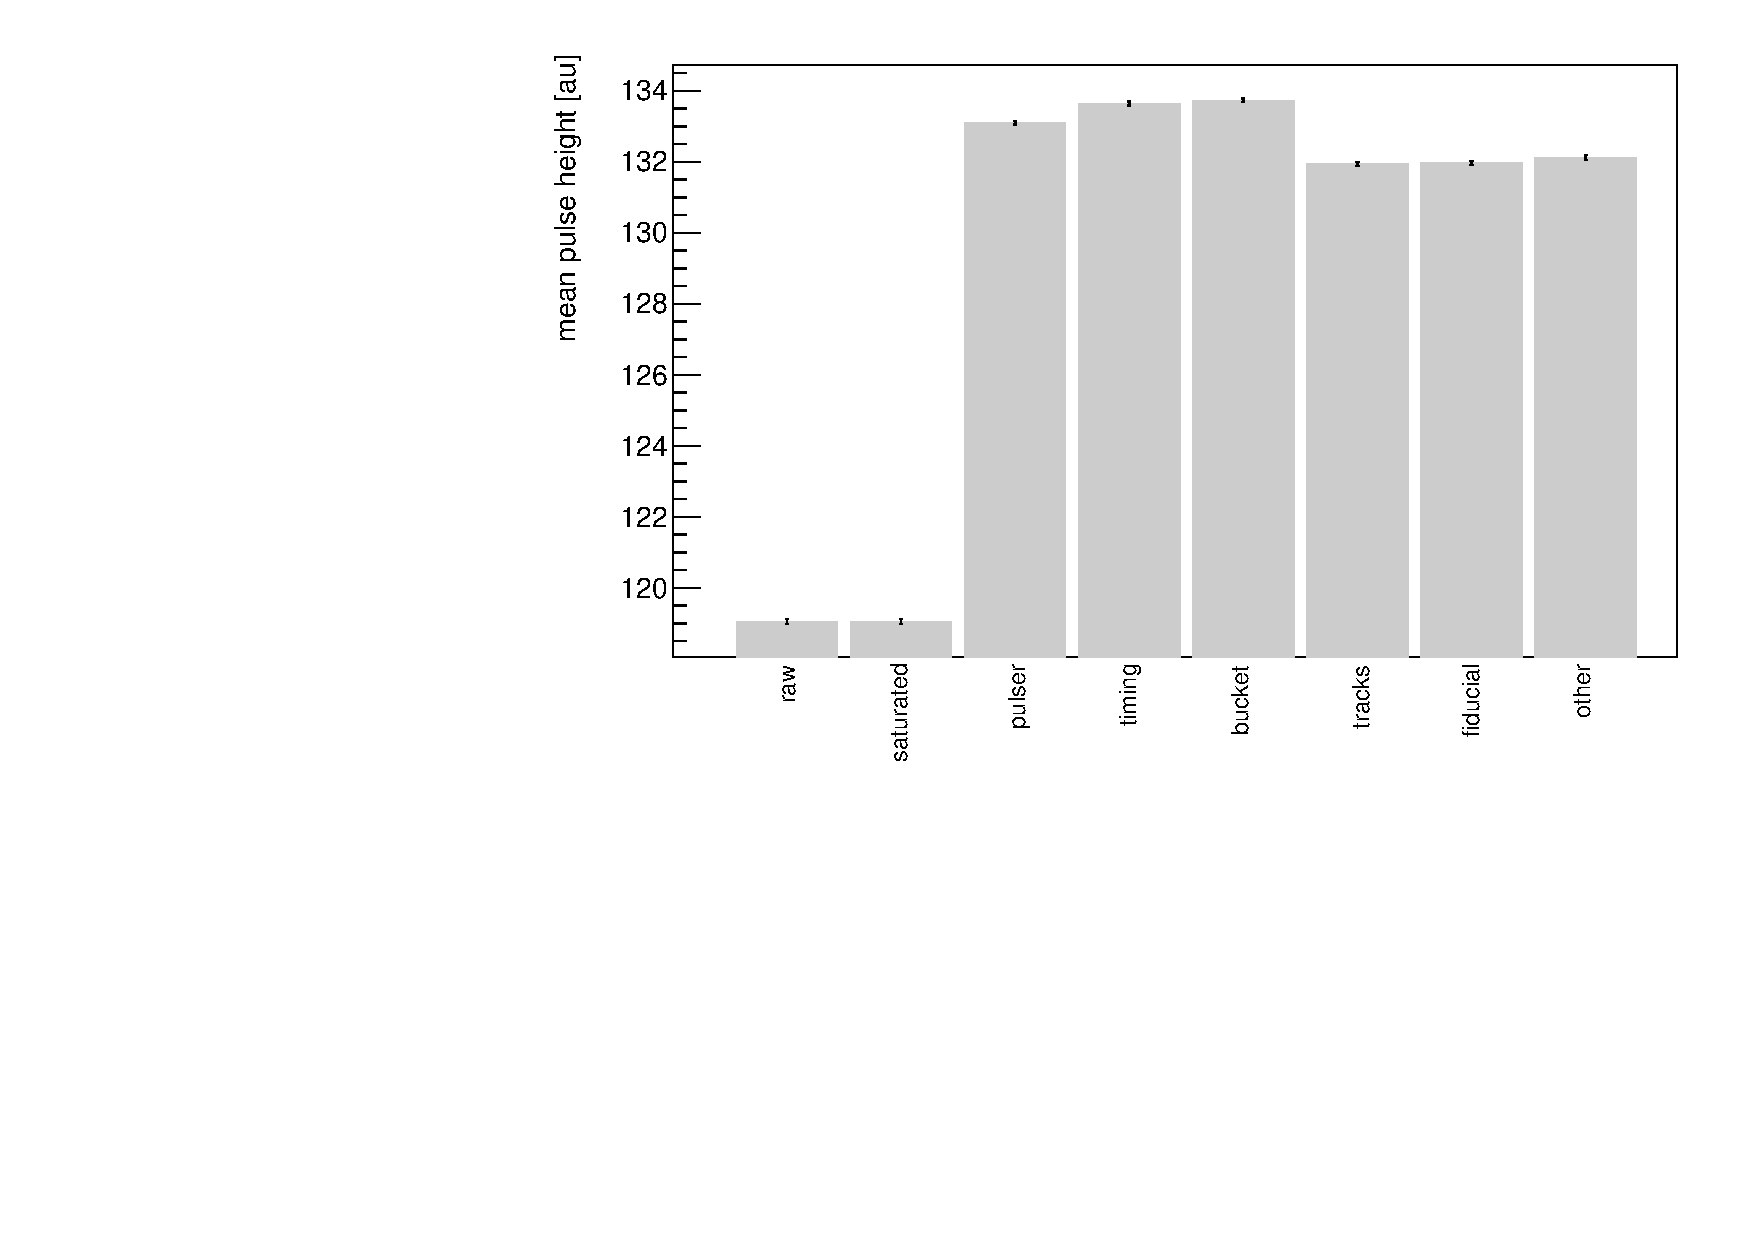
\includegraphics[angle=270, width=.7\textwidth]{CutMeans}
	\end{figure}
\end{frame}
% ============================ FRAME 27 ==========================================>
\begin{frame}
	\frametitle{Cut Contributions}
	\vspace*{-17pt}
	\begin{figure}
		\centering
		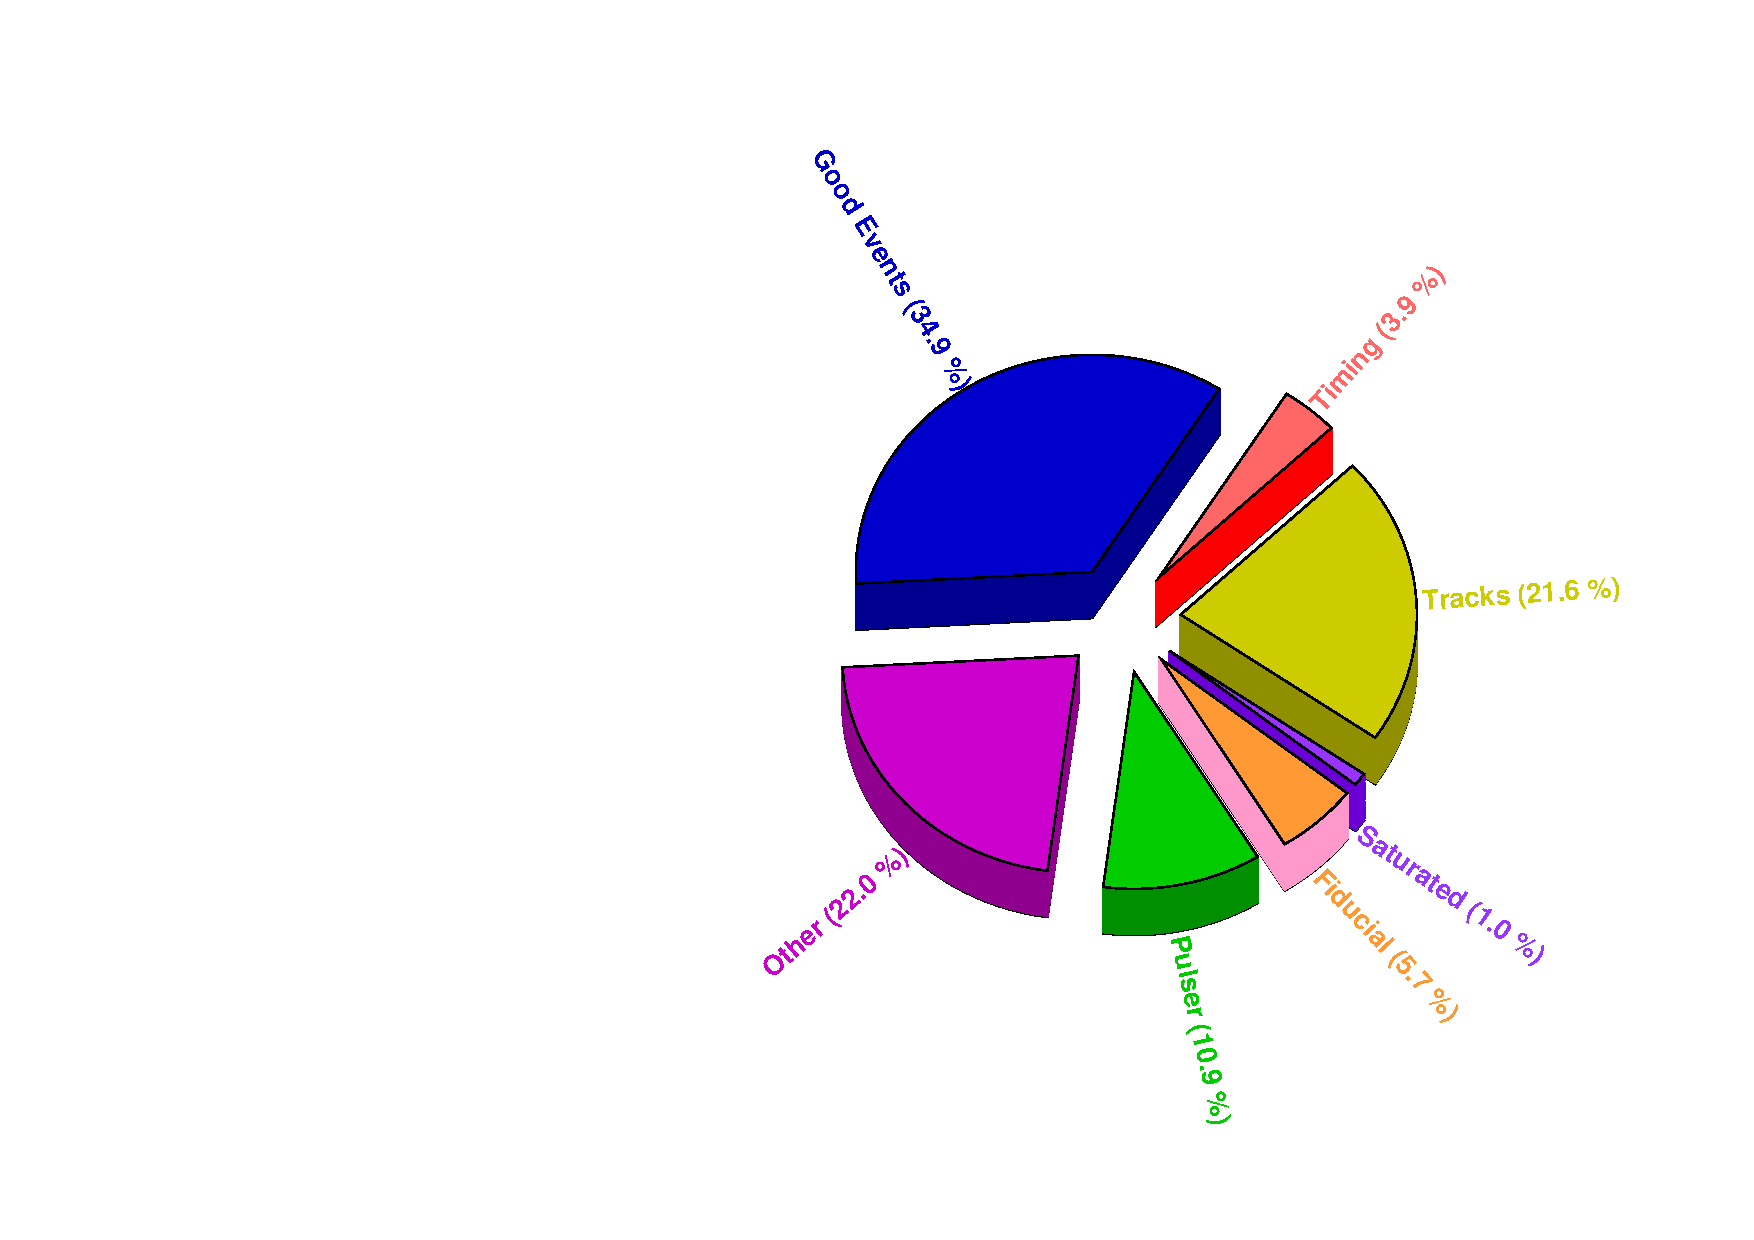
\includegraphics[angle=270, width=.6\textwidth]{CutContribution}
	\end{figure}
\end{frame}

% END 
% BEGIN RESULTS
\subsection{Results}
\begin{frame}
	\frametitle{Pulse Height Distribution and Signal Maps}
	\vspace*{-7.5pt}
	\def \sp {0.62\textwidth}
	\begin{figure}
		\centering
		\begin{subfigure}{0.45\textwidth} 
			\centering 
			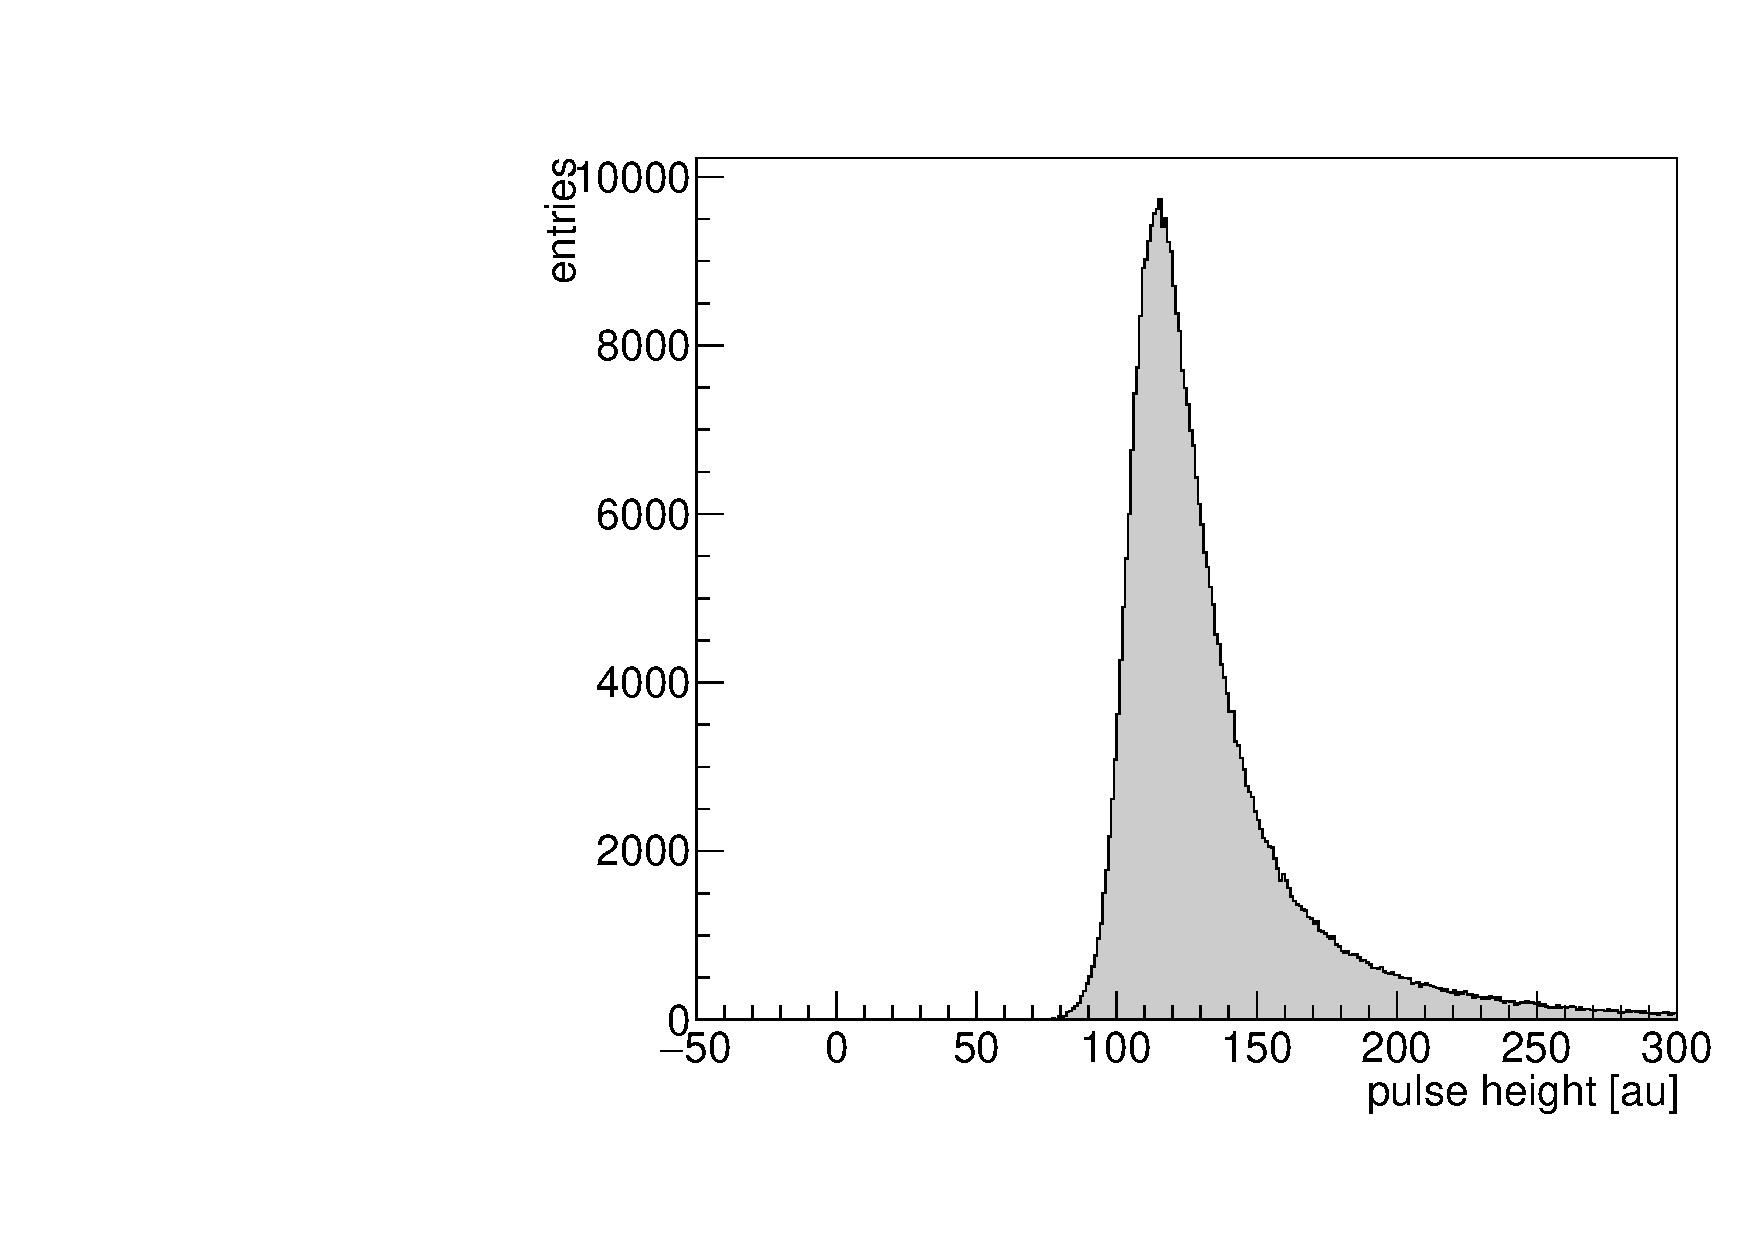
\includegraphics[angle=270, width=\sp]{sDisto}
		\end{subfigure}
		\begin{subfigure}{0.45\textwidth} 
			\centering 
			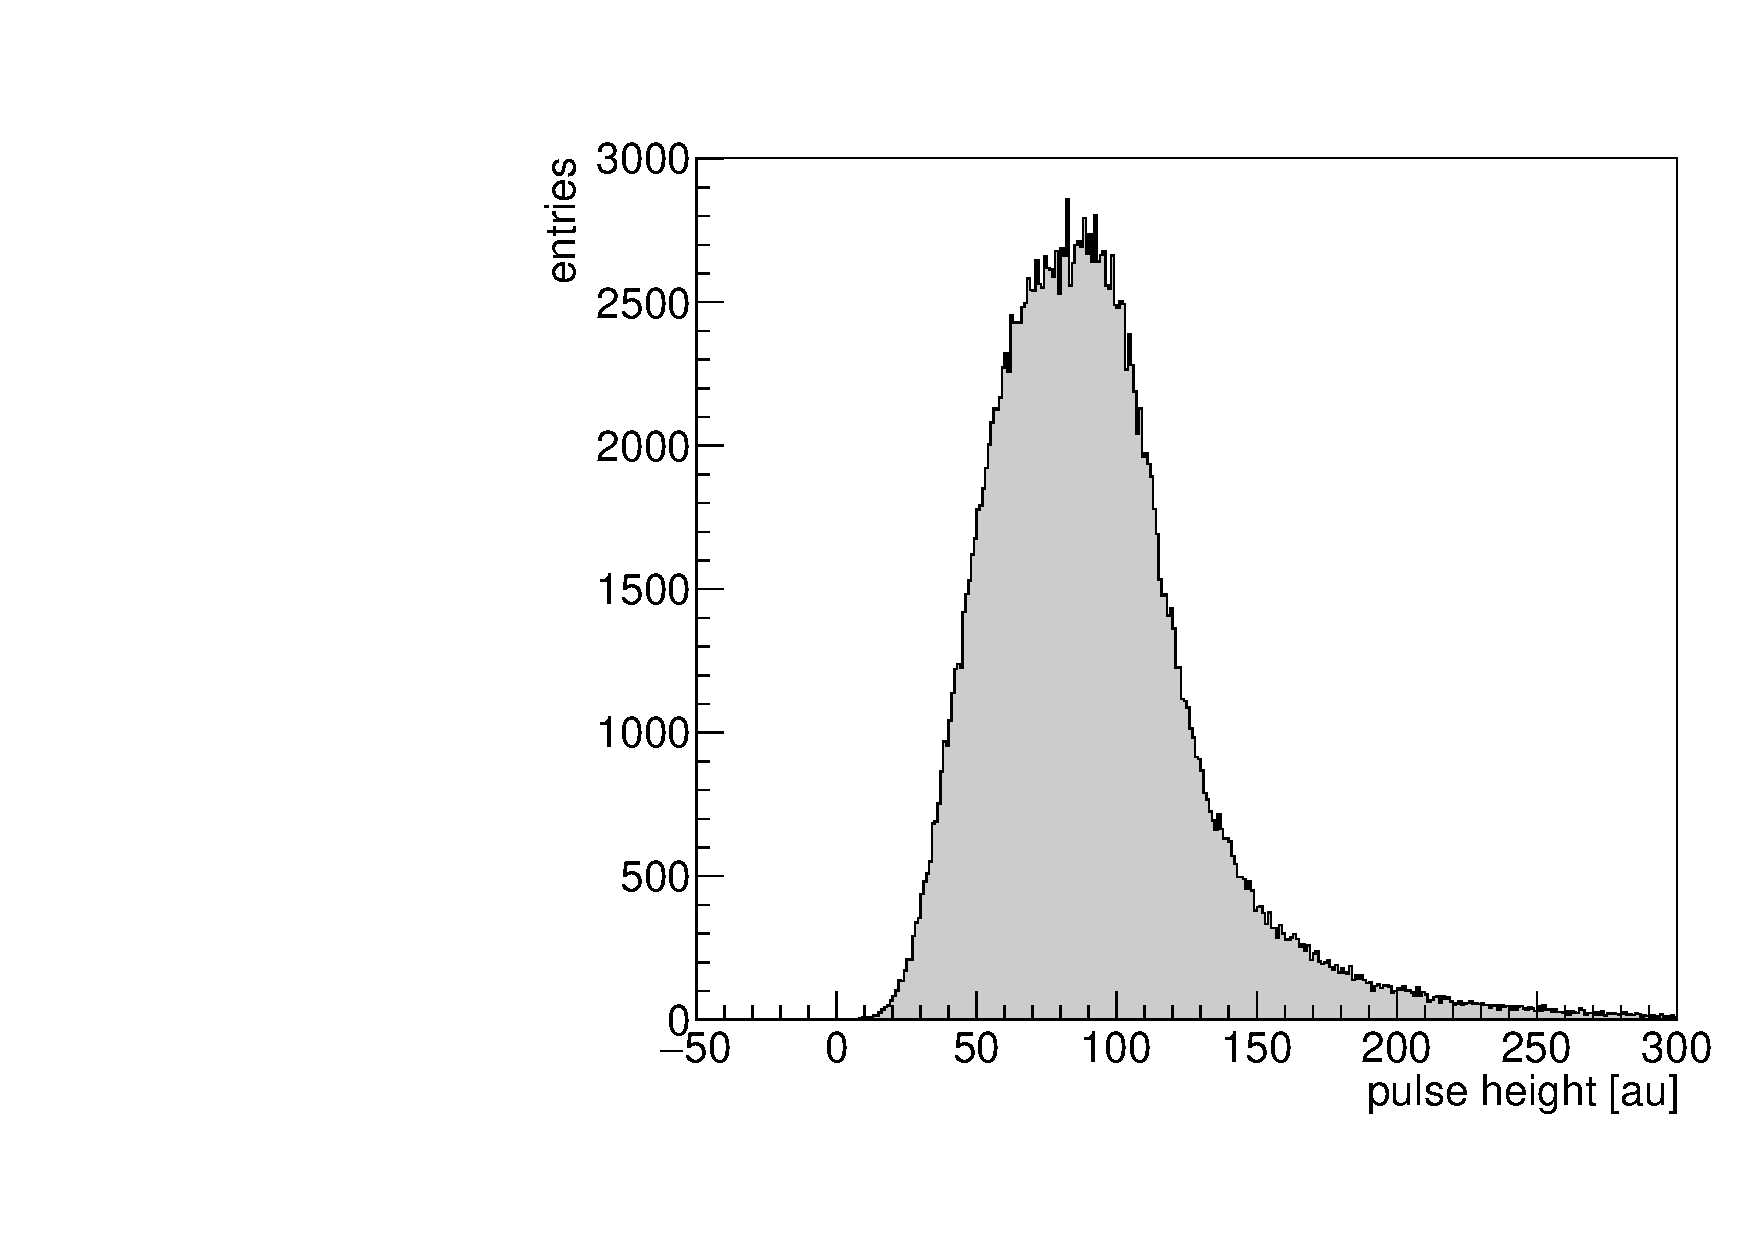
\includegraphics[angle=270, width=\sp]{pDisto}
		\end{subfigure}
	\end{figure}
	\vspace*{-15pt}
	\begin{figure}
	\centering
		\begin{subfigure}{0.45\textwidth} 
			\centering 
			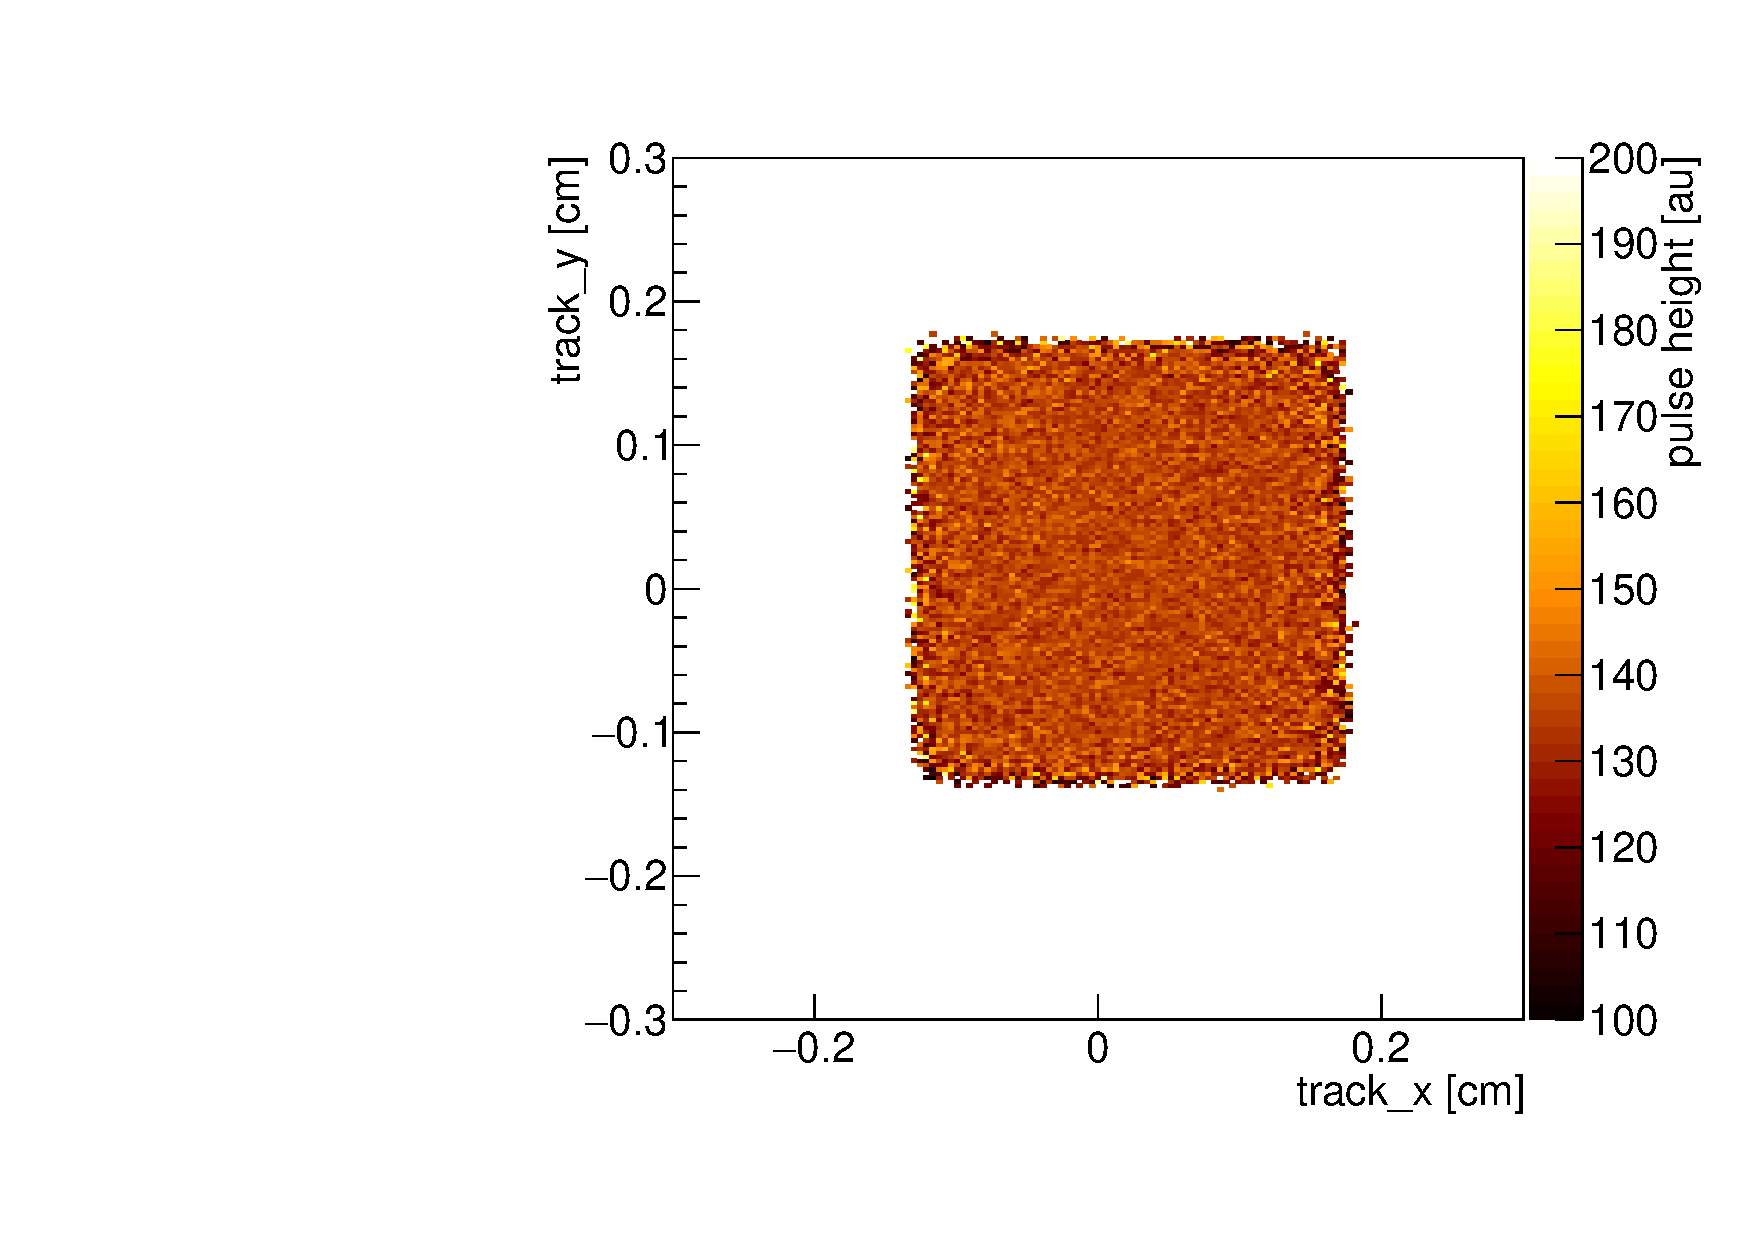
\includegraphics[angle=270, width=\sp]{sSigMap}
			\caption{single-crystalline}
		\end{subfigure}
		\begin{subfigure}{0.45\textwidth} 
			\centering 
			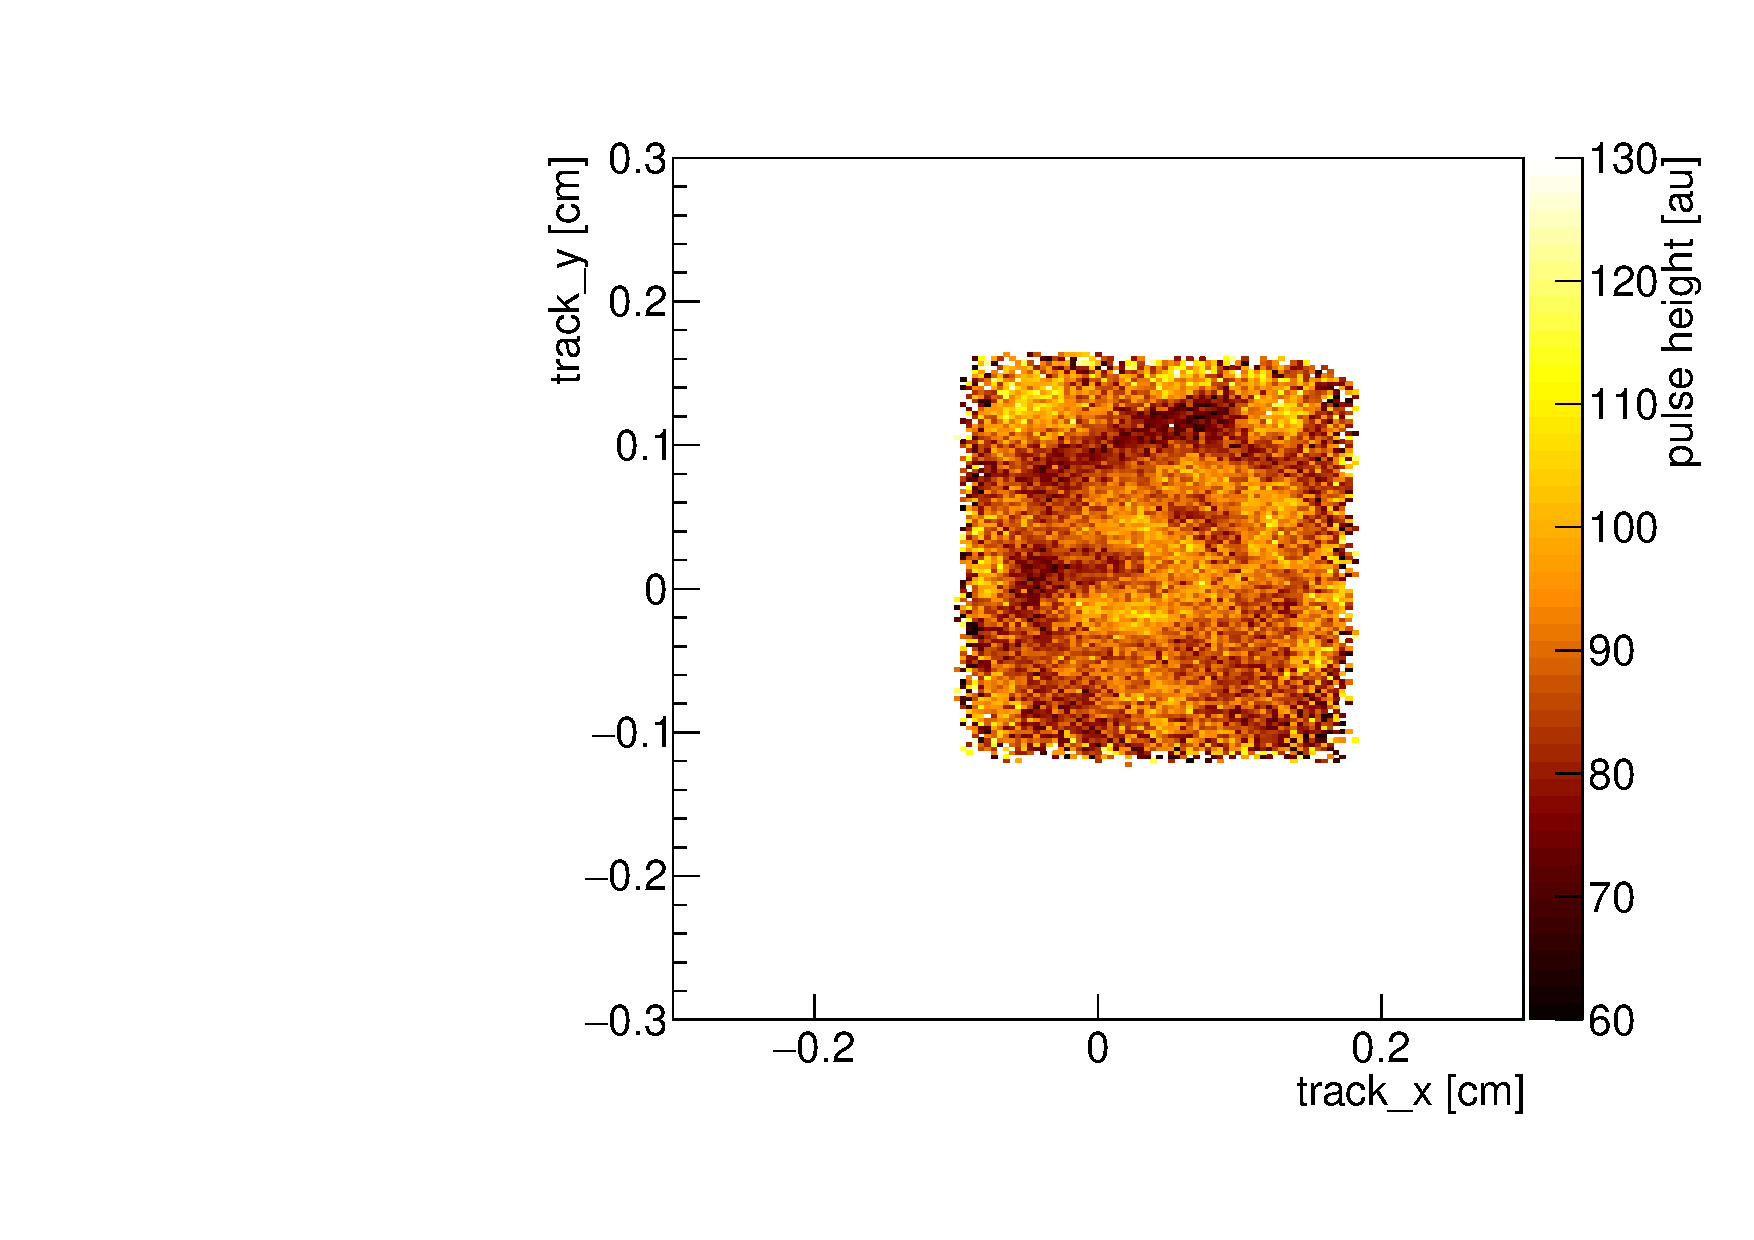
\includegraphics[angle=270, width=\sp]{pSigMap}
			\caption{poly-crystalline}
		\end{subfigure} 
	\end{figure}
\end{frame}
% ============================ new frame ==========================================>
\begin{frame}
	\frametitle{Signal vs. Particle Flux}
	\begin{minipage}[c][.75\textheight]{.5\textwidth}
		\begin{itemize}
			\setlength{\itemsep}{\fill}
			\item after all analysis steps: look for rate dependence of pCVD diamonds
			\item found diamond pad detectors that show no or very little dependence on rate
			\item no dependence up to \SI{1e16}{neq\per cm^2}
			\item large systematic errors due to reproducibility
		\end{itemize}
		\vspace*{3pt}
		\textbf{To do:}
		\begin{itemize}
			\setlength{\itemsep}{\fill}
			\item test higher irradiated samples
			\item improve reproducibility
			\item prove the same for pixel detectors
		\end{itemize}
	\end{minipage}
	\hspace*{5pt}
	\begin{minipage}{.45\textwidth}
		\begin{figure}
			\centering
			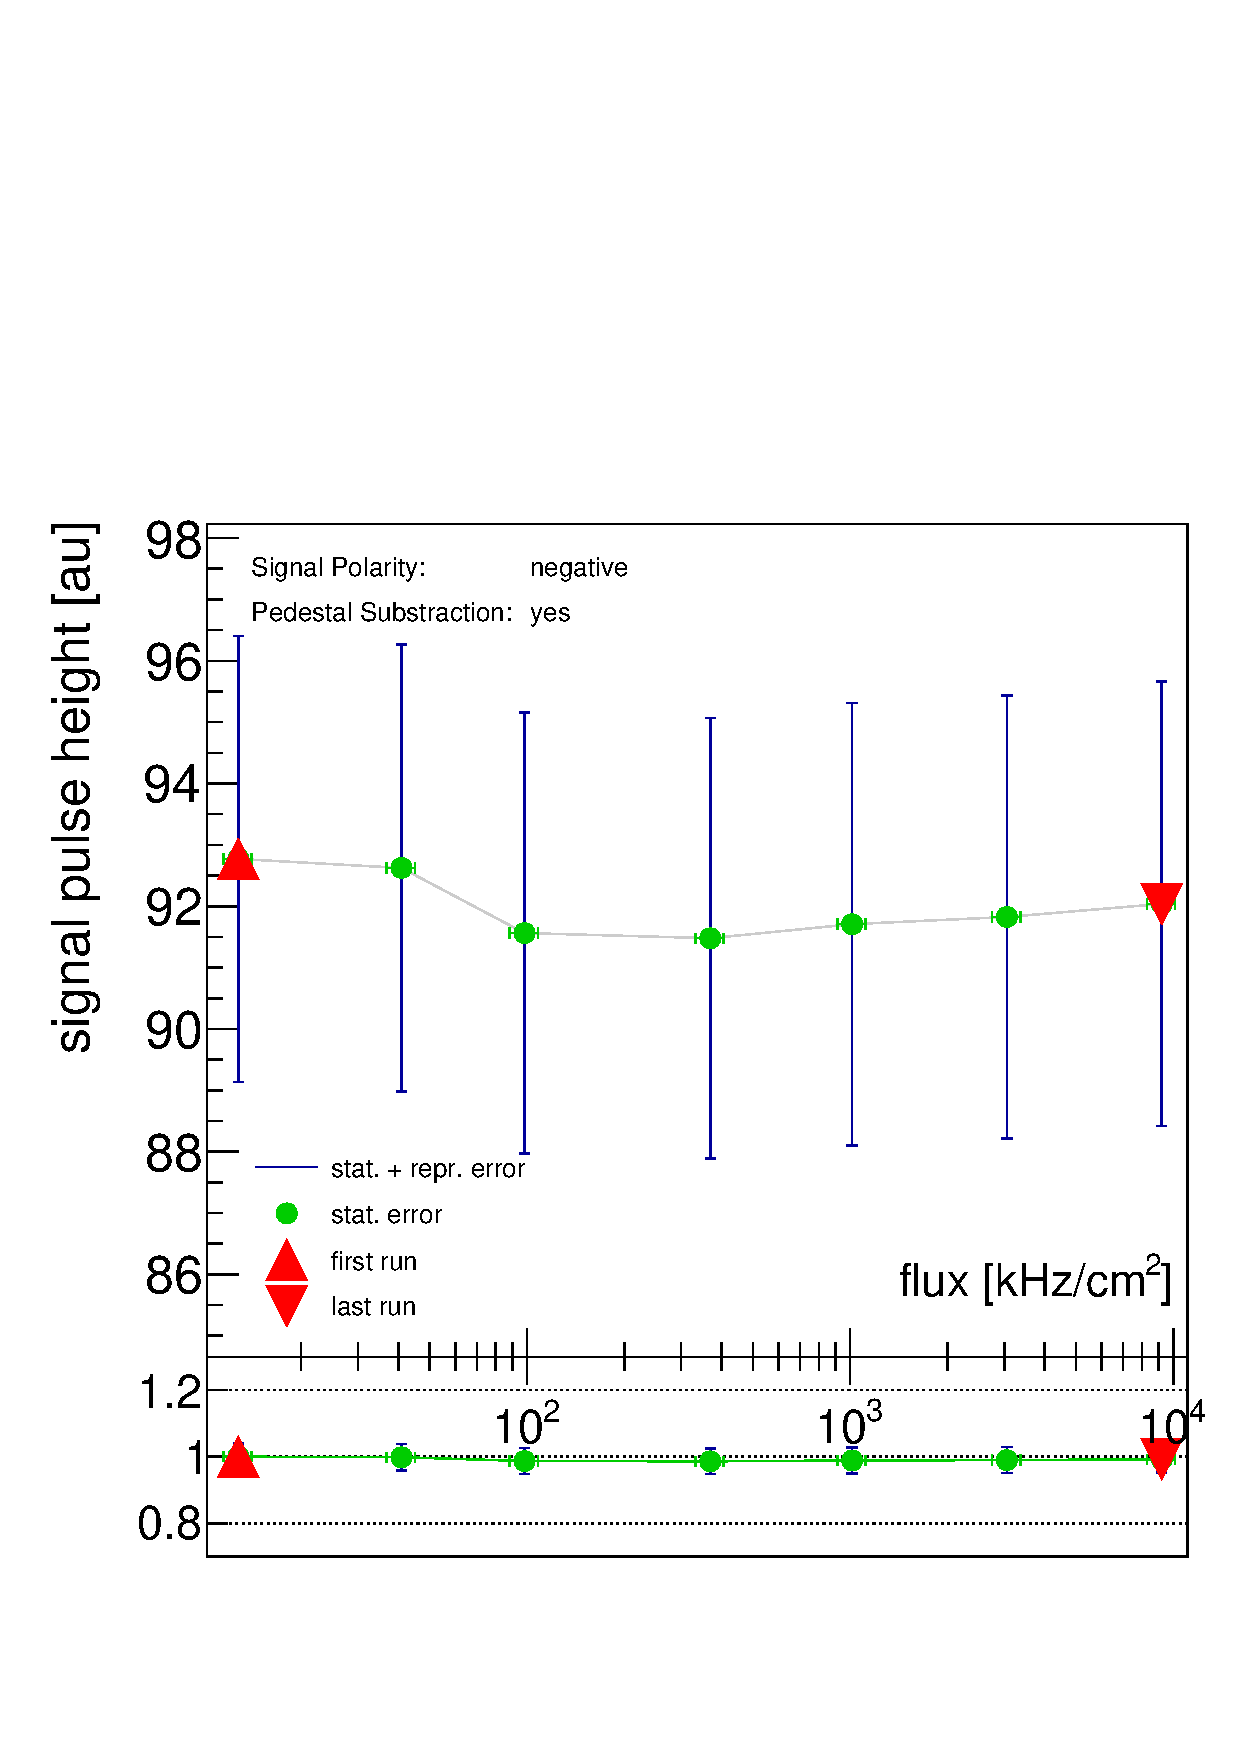
\includegraphics[width=\textwidth]{rateplot}
		\end{figure}
	\end{minipage}
\end{frame}
% ============================ new frame ==========================================>
\begin{frame}
	\frametitle{Single crystalline diamond}
	\def \sp {3.7cm}
	\begin{minipage}{\sp}
		\centering
		October 2015 
		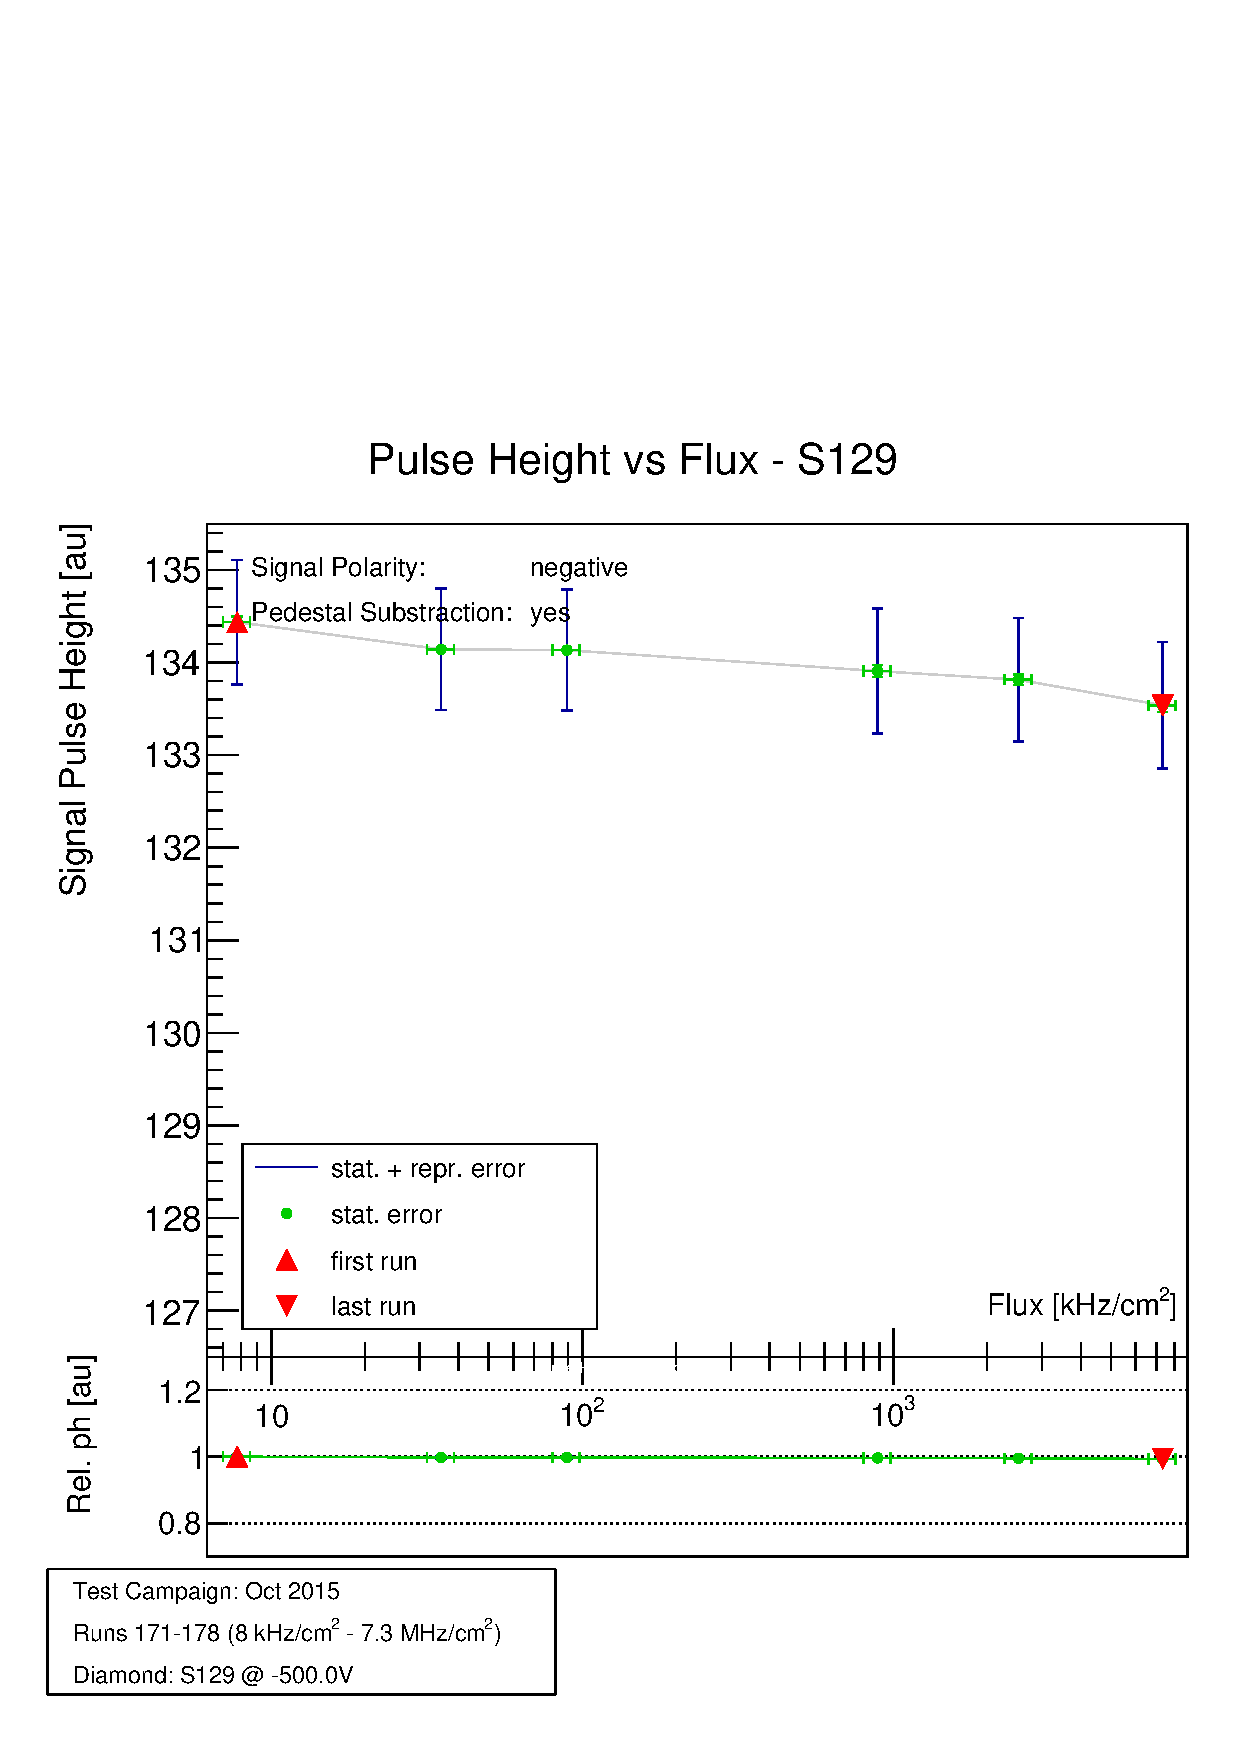
\includegraphics[width=\sp]{CPH1608_03}\\
		noise $\upsigma\approx$ \SI{2.6}{au}
	\end{minipage}
	\hspace*{2pt}
	\begin{minipage}{\sp}
		\centering
		August 2016 - begin
		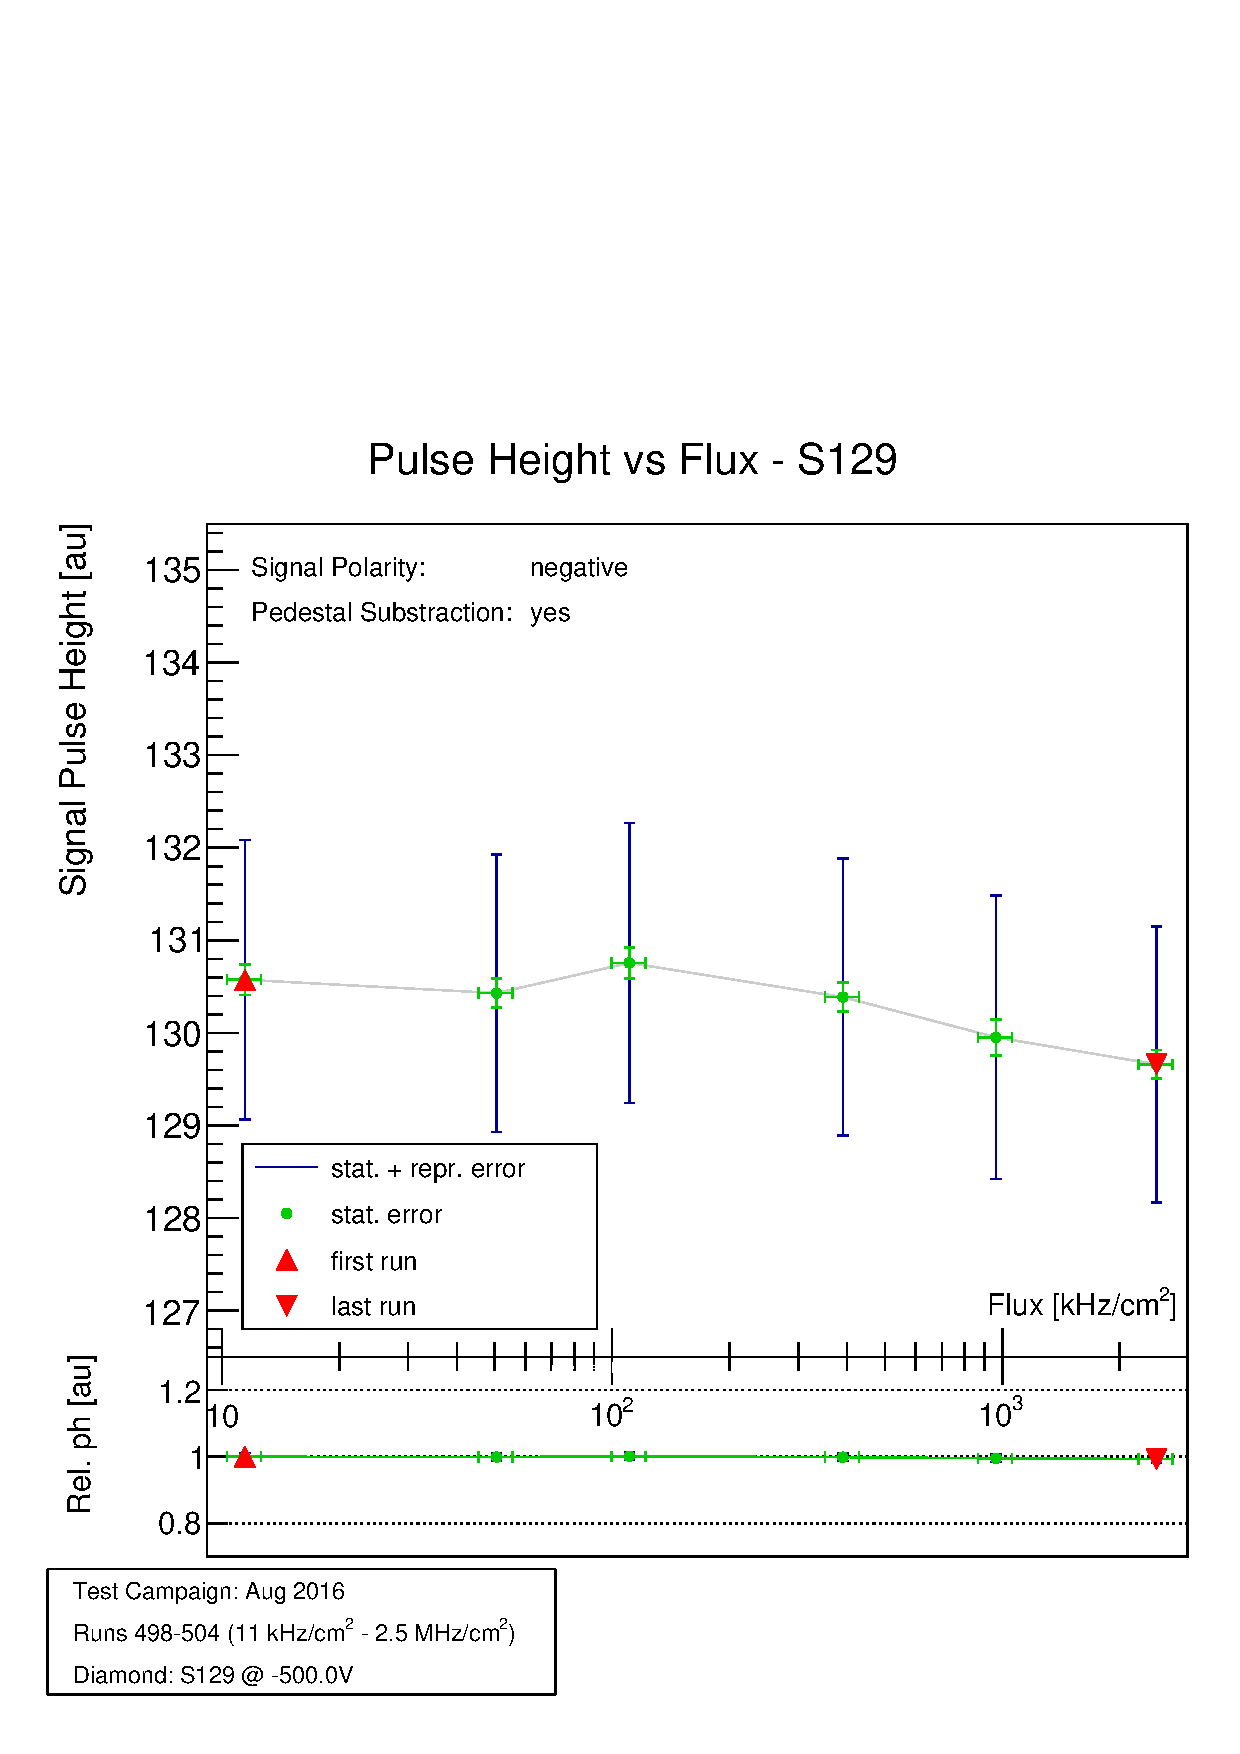
\includegraphics[width=\sp]{CPH1510_08_1}\\
		noise $\upsigma\approx$ \SI{2.6}{au}
	\end{minipage}
	\hspace*{2pt}
	\begin{minipage}{\sp}
		\centering
		August 2016 - end
		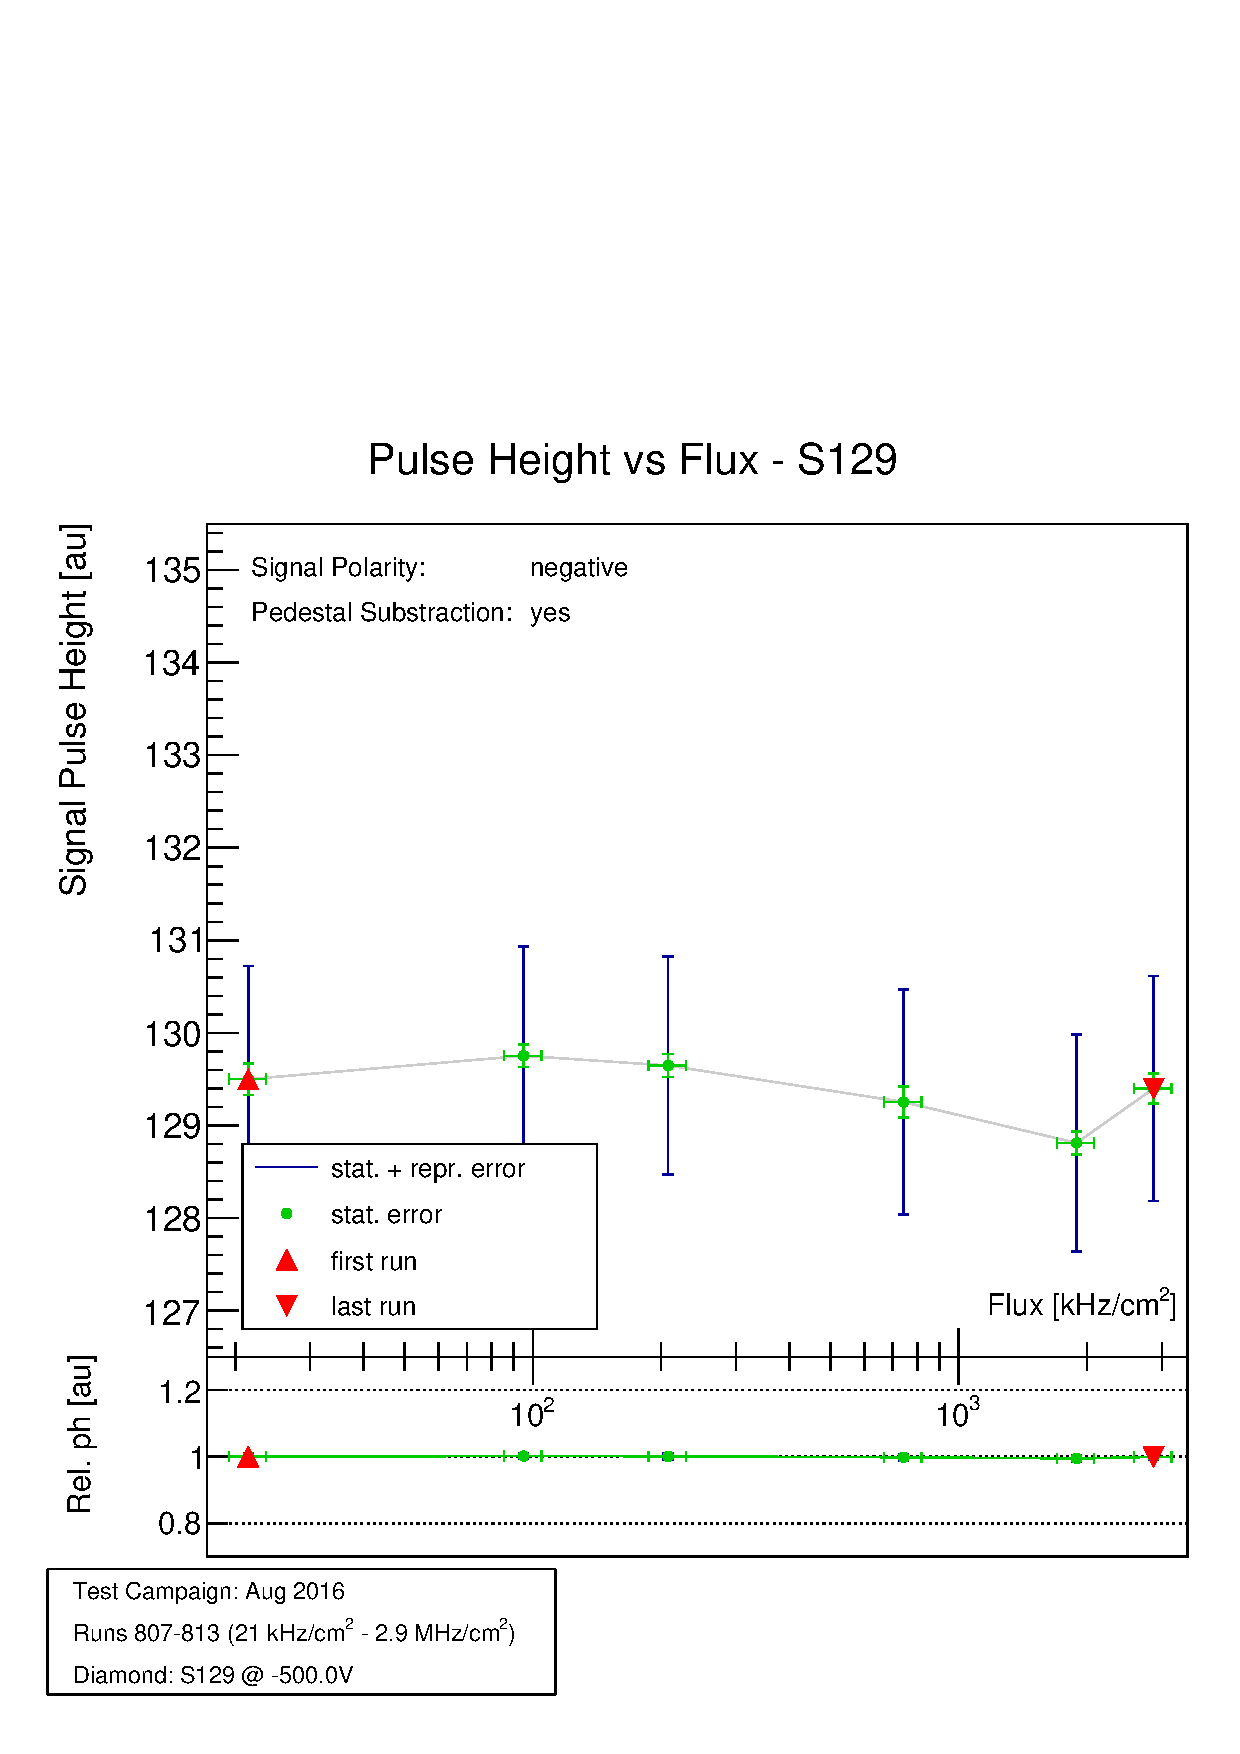
\includegraphics[width=\sp]{CPH1510_18_1}\\
		noise $\upsigma \approx$ \SI{2.6}{au}
	\end{minipage}\s
	\begin{itemize}
		\item measurements taken under the same conditions
		\item noise stays the same
		\item pulse height very stable
	\end{itemize}
\end{frame}
% ============================ new frame ==========================================>
\begin{frame}
	\frametitle{Poly crystalline diamond}
	\begin{minipage}{3.7cm}
		\centering
		August 2016 - \\unirradiated
		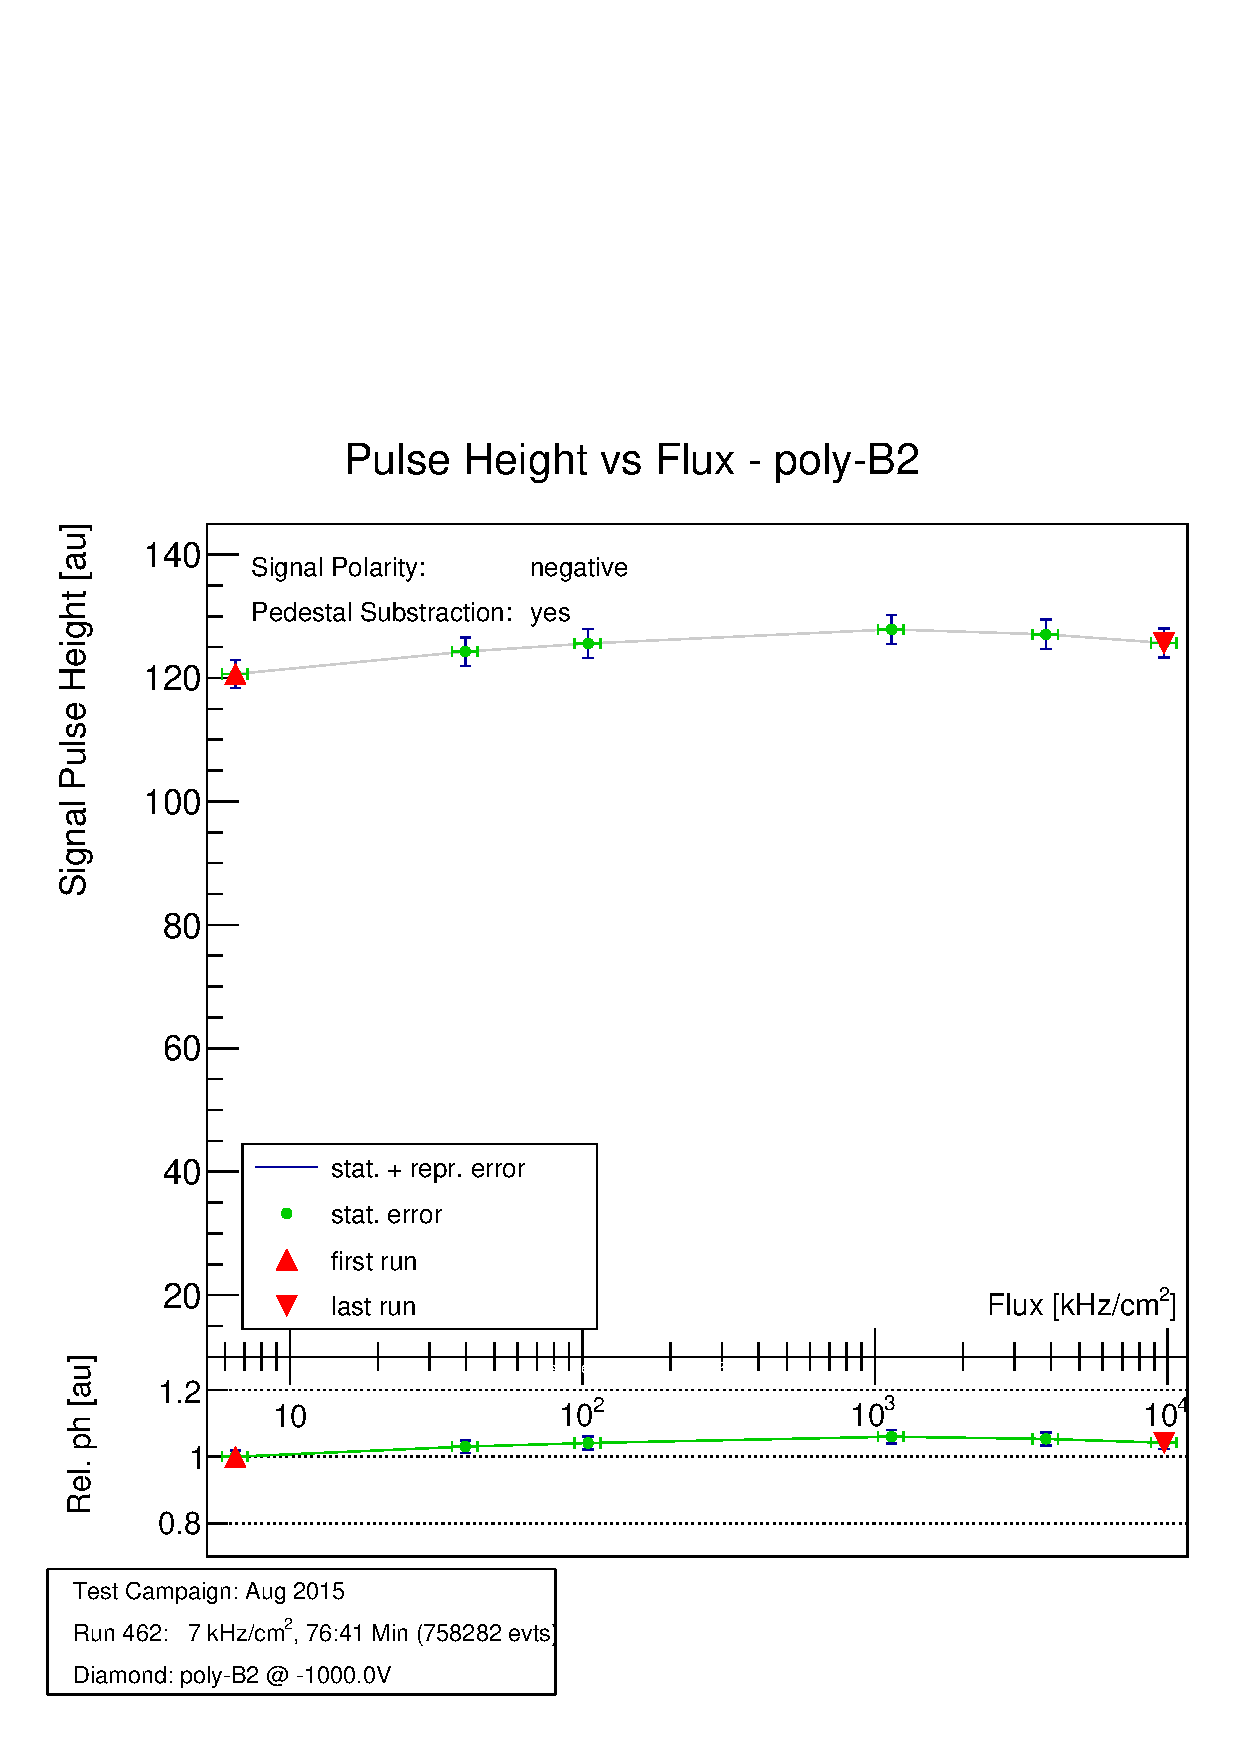
\includegraphics[width=3.7cm]{CPH1508_13_2.pdf}\\
		noise $\upsigma\approx$ \SI{4.9}{au}
	\end{minipage}
	\hspace*{2pt}
	\begin{minipage}{3.7cm}
		\centering
		October 2015 - \SI[exponent-product = \cdot]{5e14}{n/cm^{2}}
		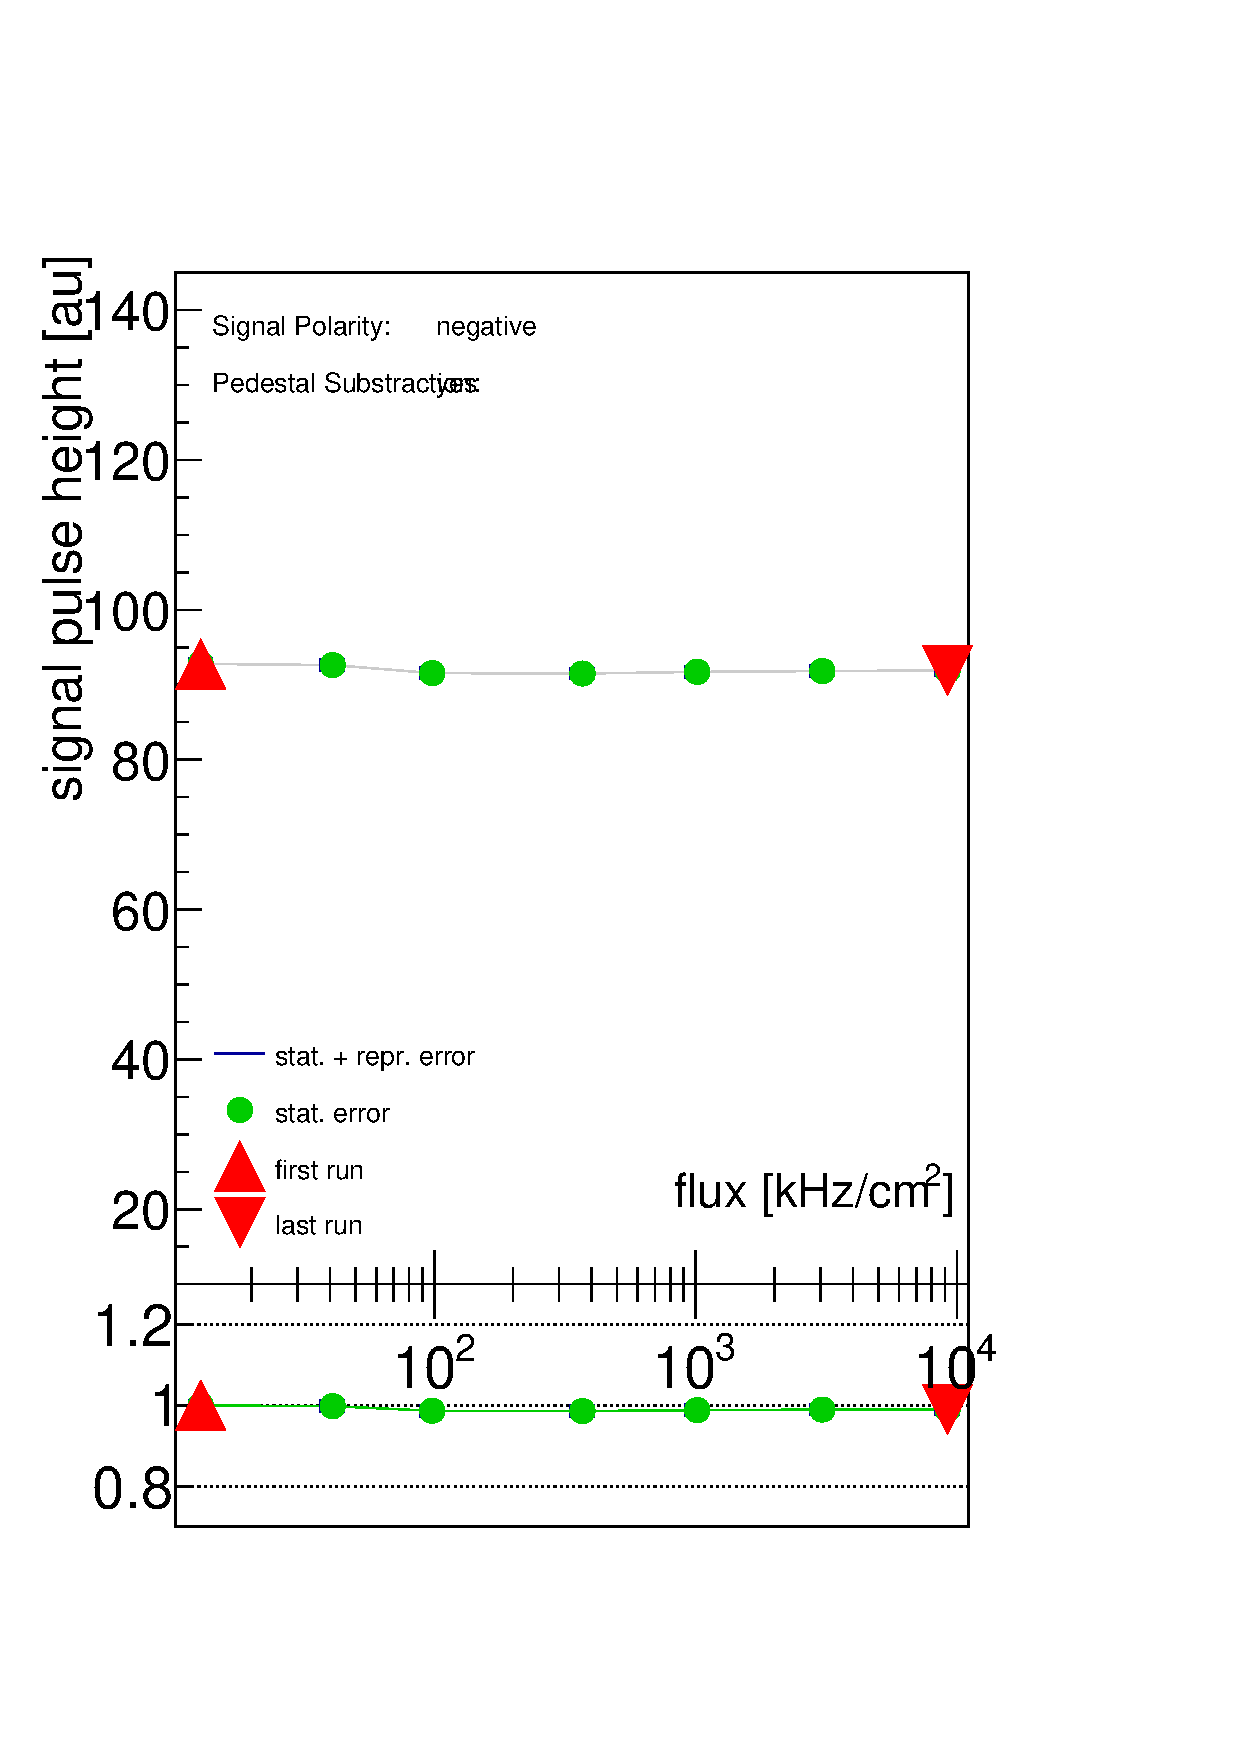
\includegraphics[width=3.7cm]{CPH1510_08_2.pdf}\\
		noise $\upsigma\approx$ \SI{4.9}{au}
	\end{minipage}
	\hspace*{2pt}
	\begin{minipage}{3.7cm}
		\centering
		August 2016 - \SI[exponent-product = \cdot]{1e15}{n/cm^{2}}
		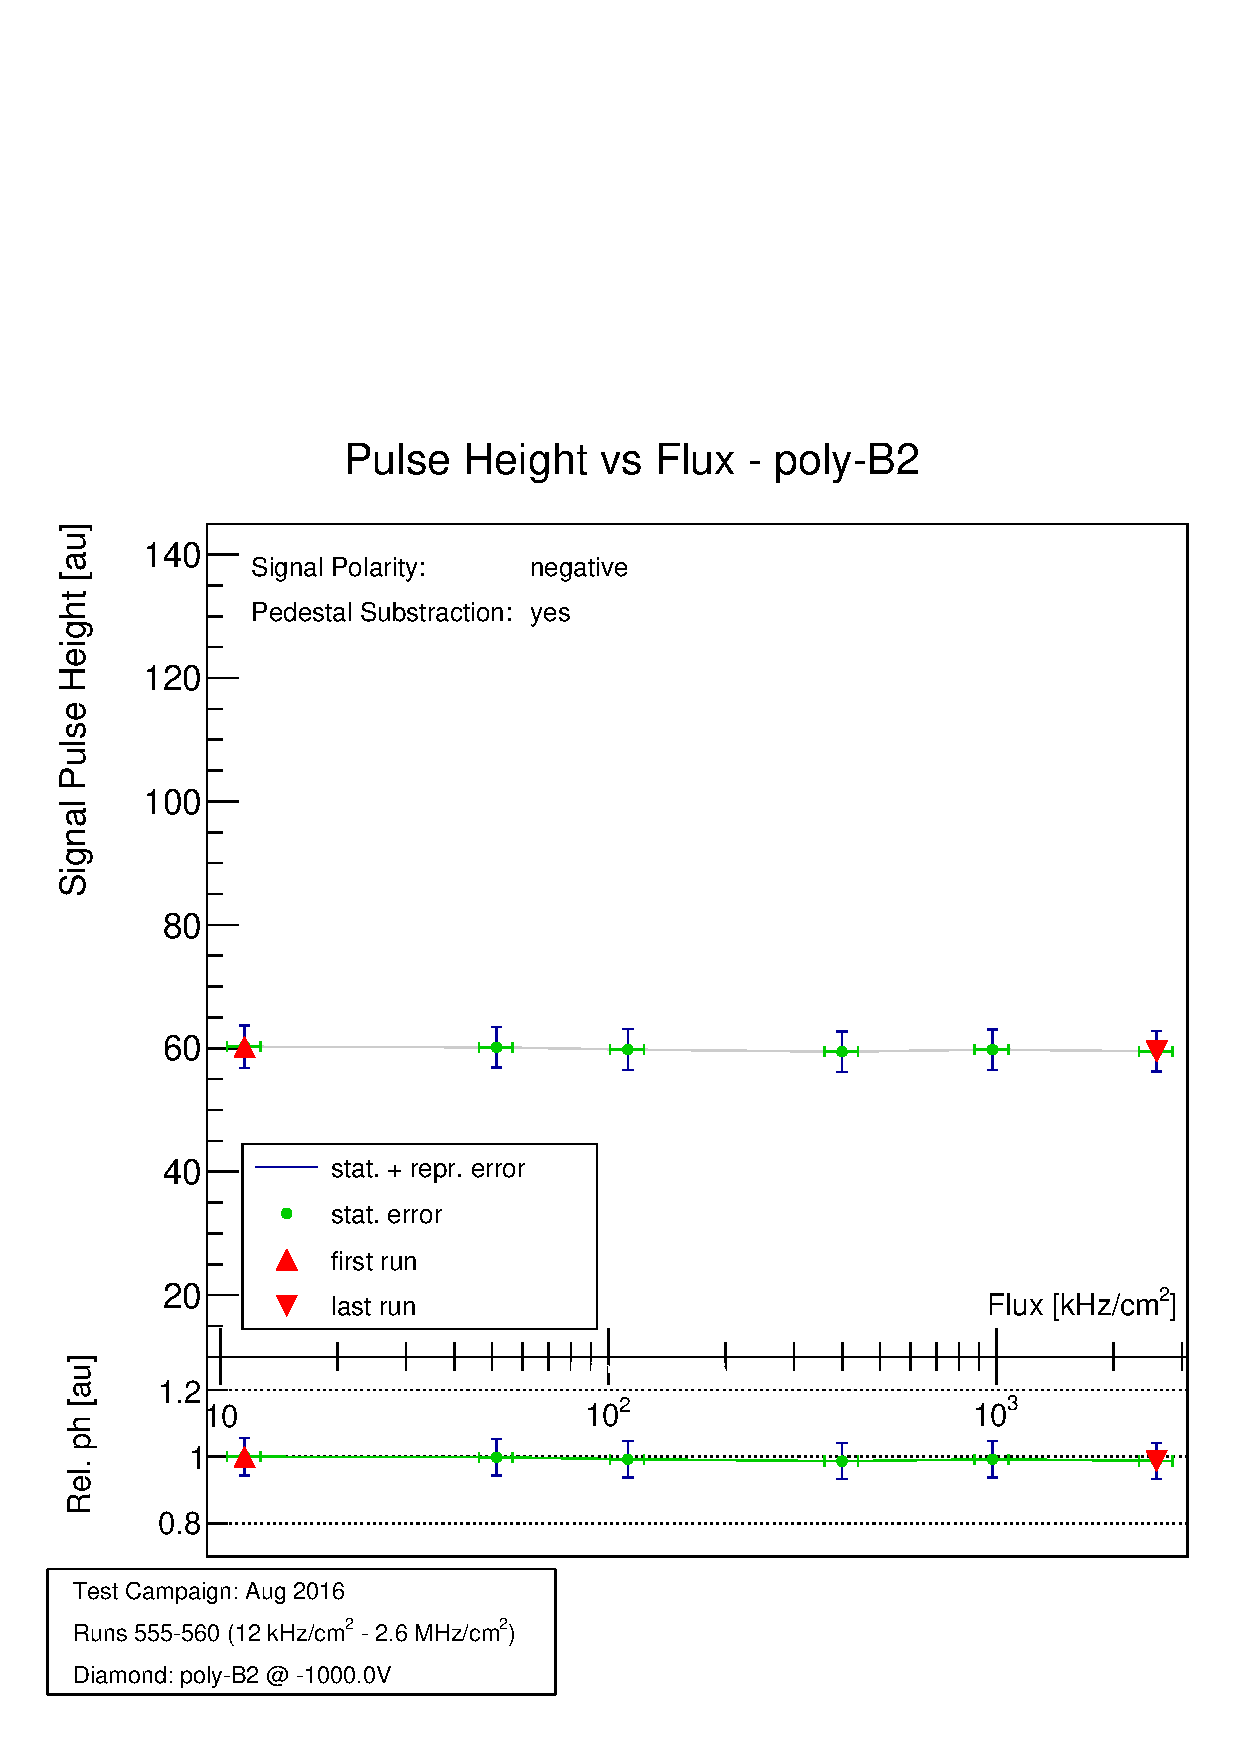
\includegraphics[width=3.7cm]{CPH1608_09_1_2.pdf}\\
		noise $\upsigma \approx$ \SI{4.9}{au}
	\end{minipage}\s
	\begin{itemize}
		\item pulse height very stable after irradiation
		\item noise stays the same
	\end{itemize}
\end{frame}
% ============================ new frame ==========================================>
\begin{frame}
	\begin{minipage}{3.1cm}
		\centering
		August 2016 - \\unirradiated
		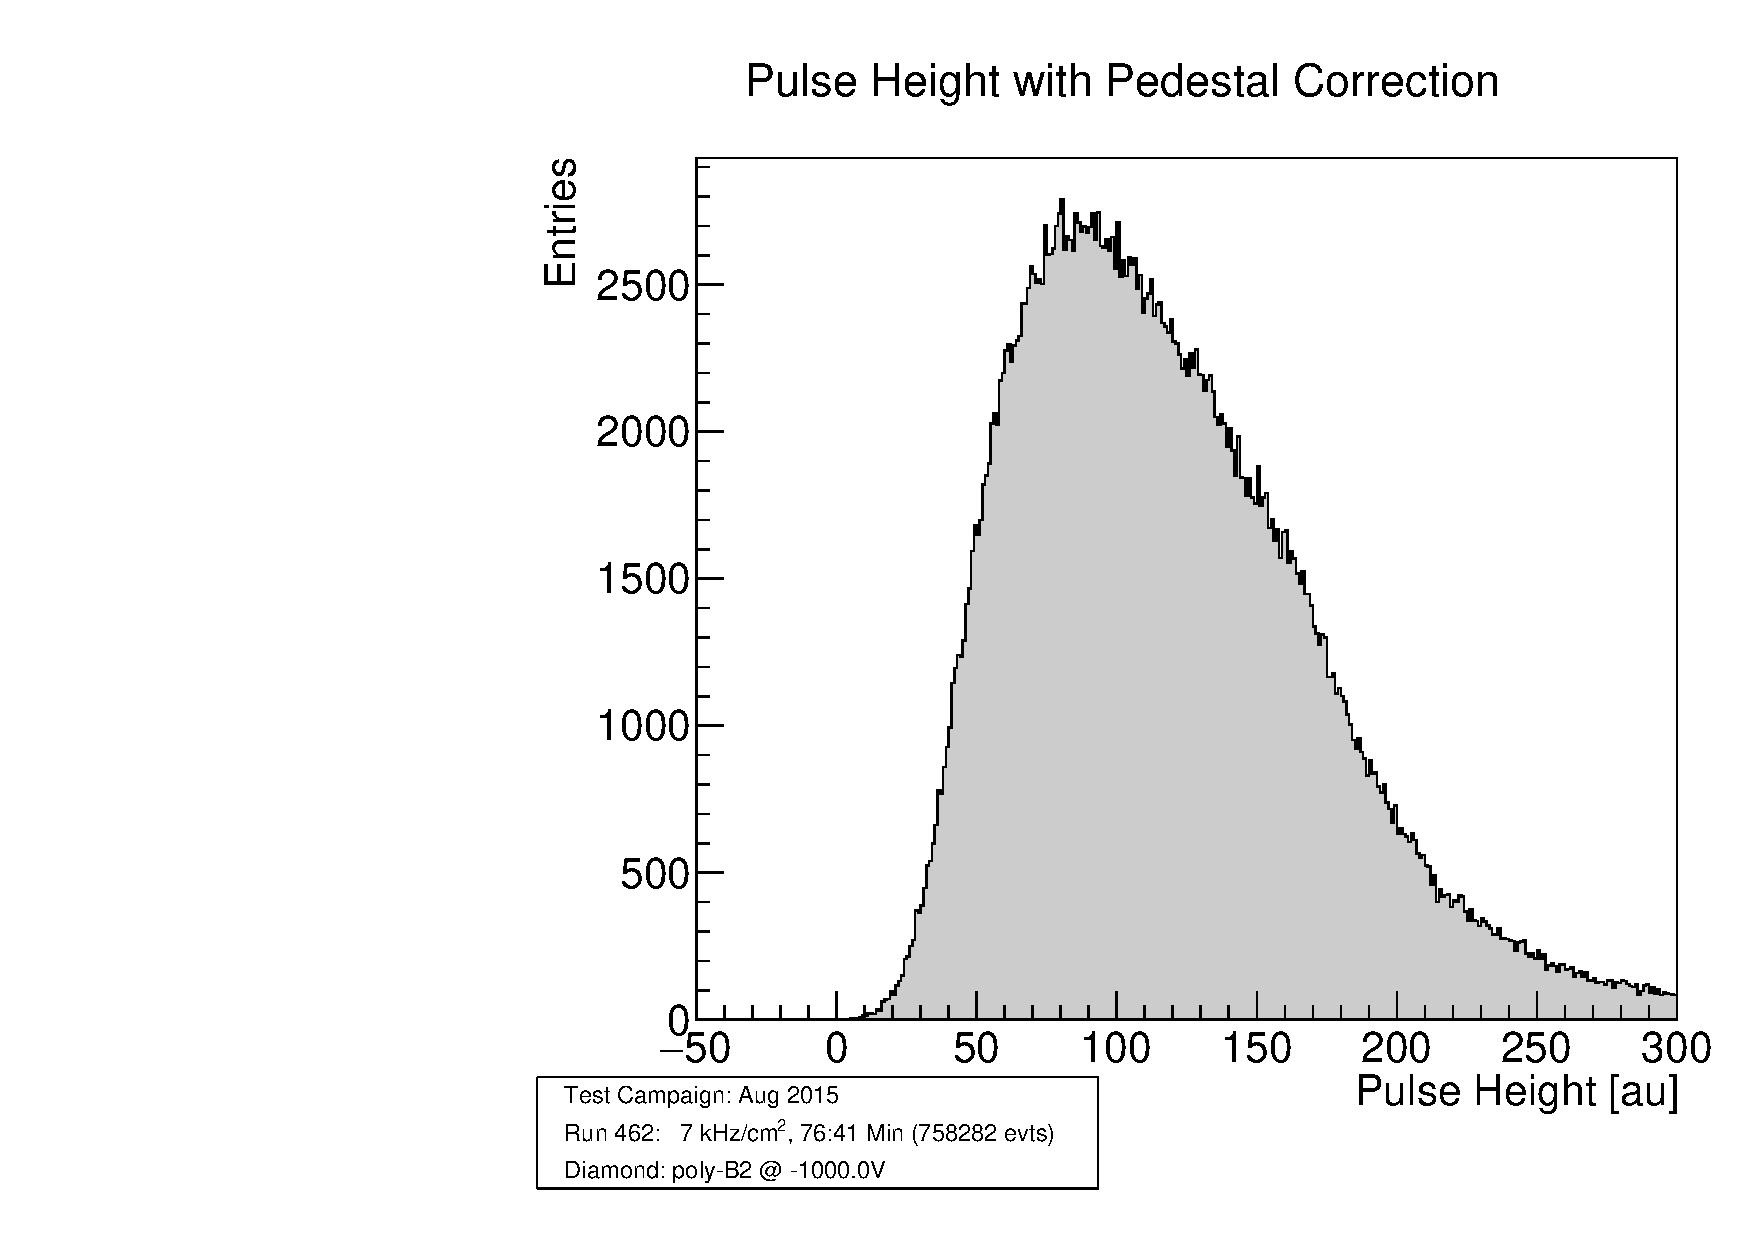
\includegraphics[angle=270, width=3.1cm]{SD462}\\
		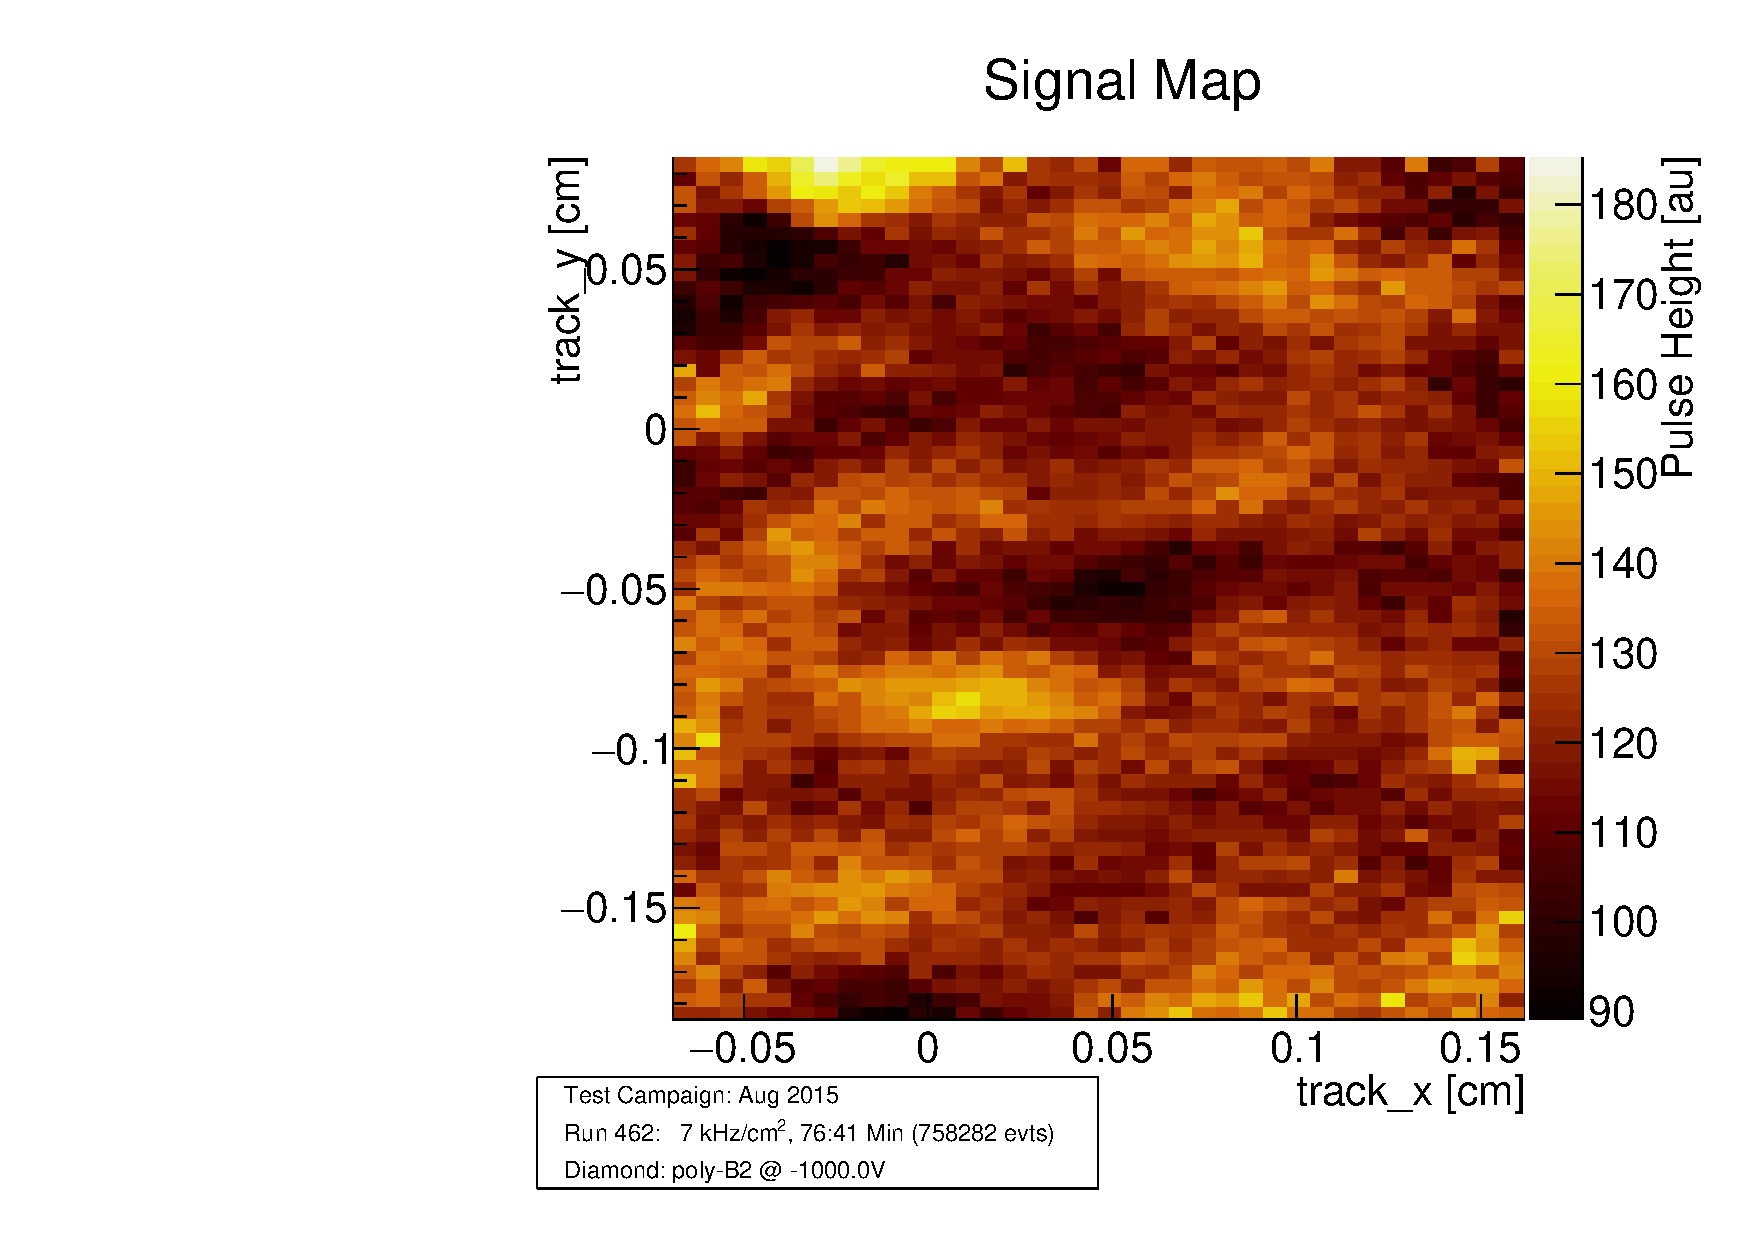
\includegraphics[angle=270, width=3.1cm]{SM462}
	\end{minipage}
	\hspace*{2pt}
	\begin{minipage}{3.1cm}
		\centering
		October 2015 - \SI[exponent-product = \cdot]{5e14}{n/cm^{2}}
		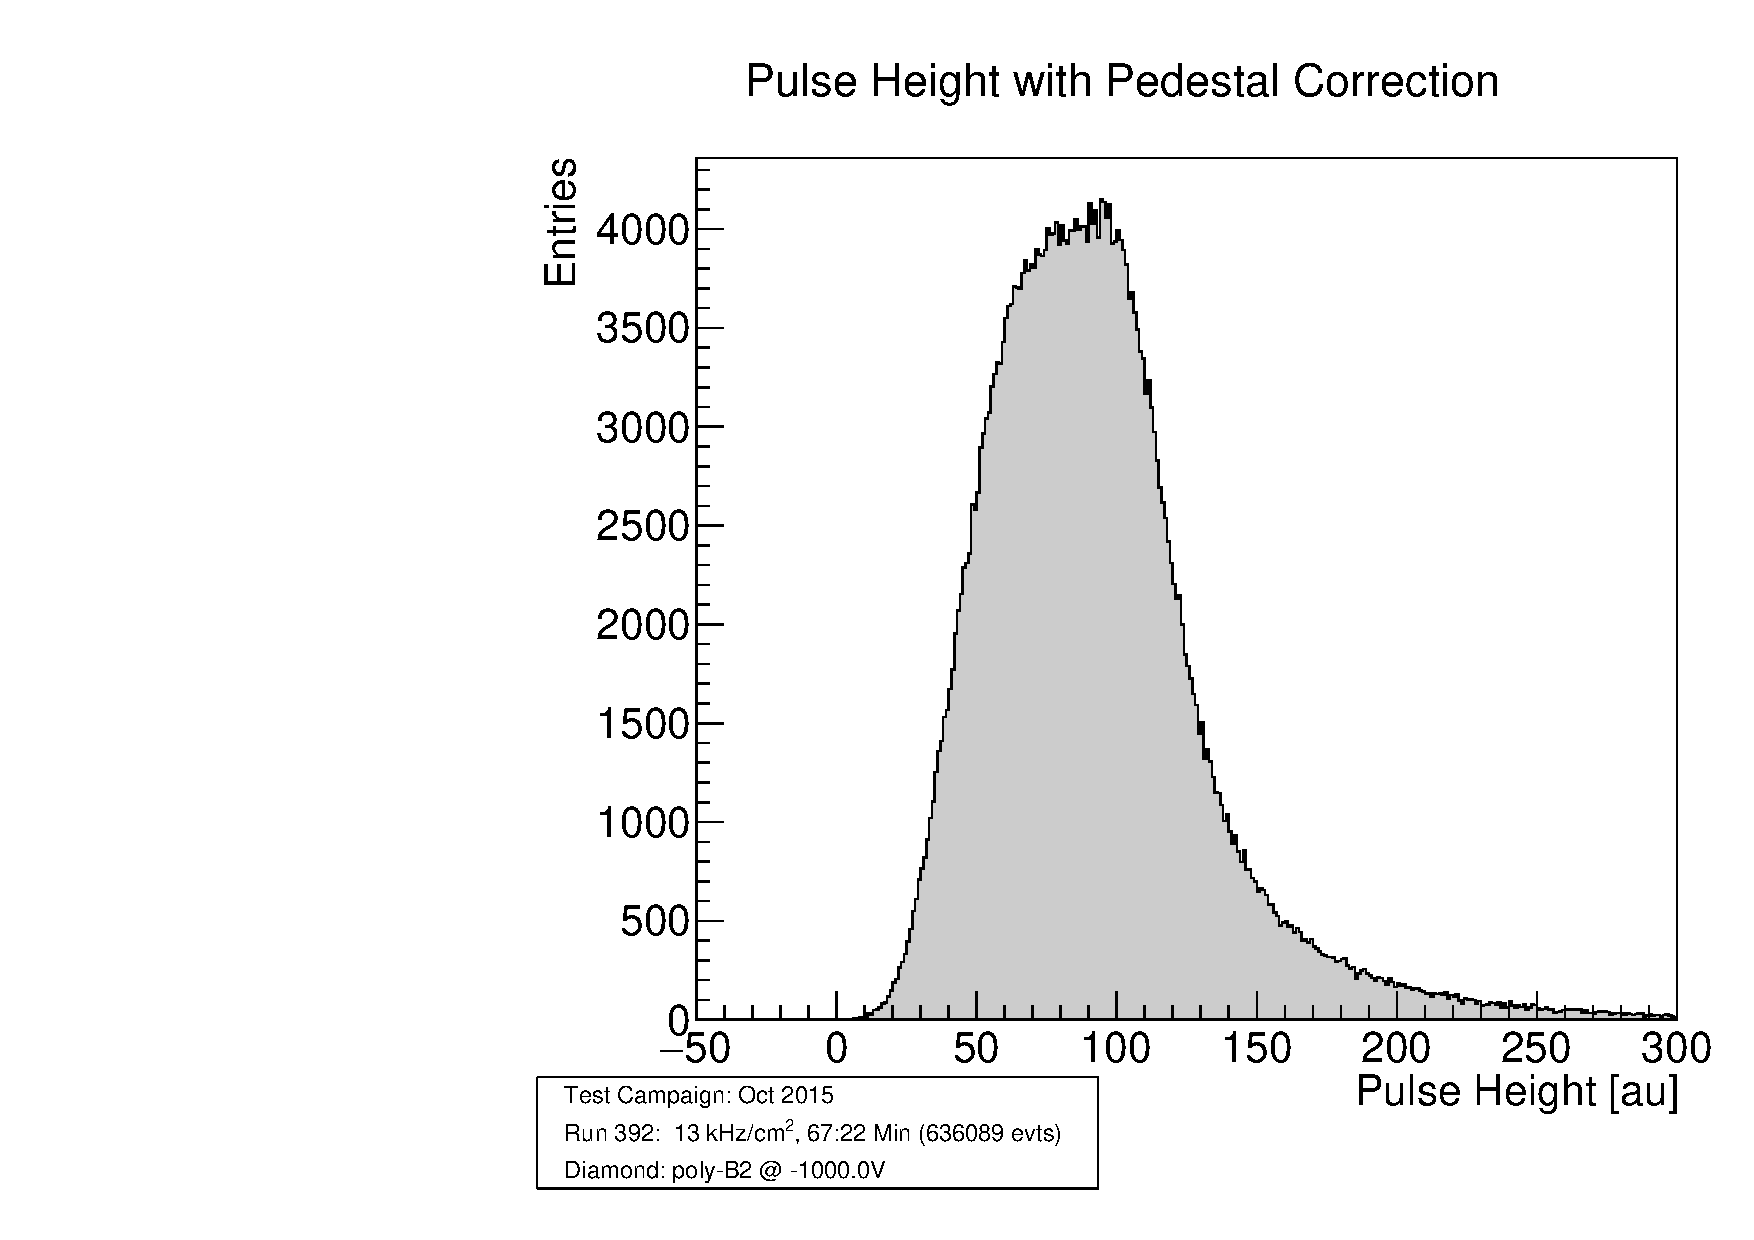
\includegraphics[angle=270, width=3.1cm]{SD392}\\
		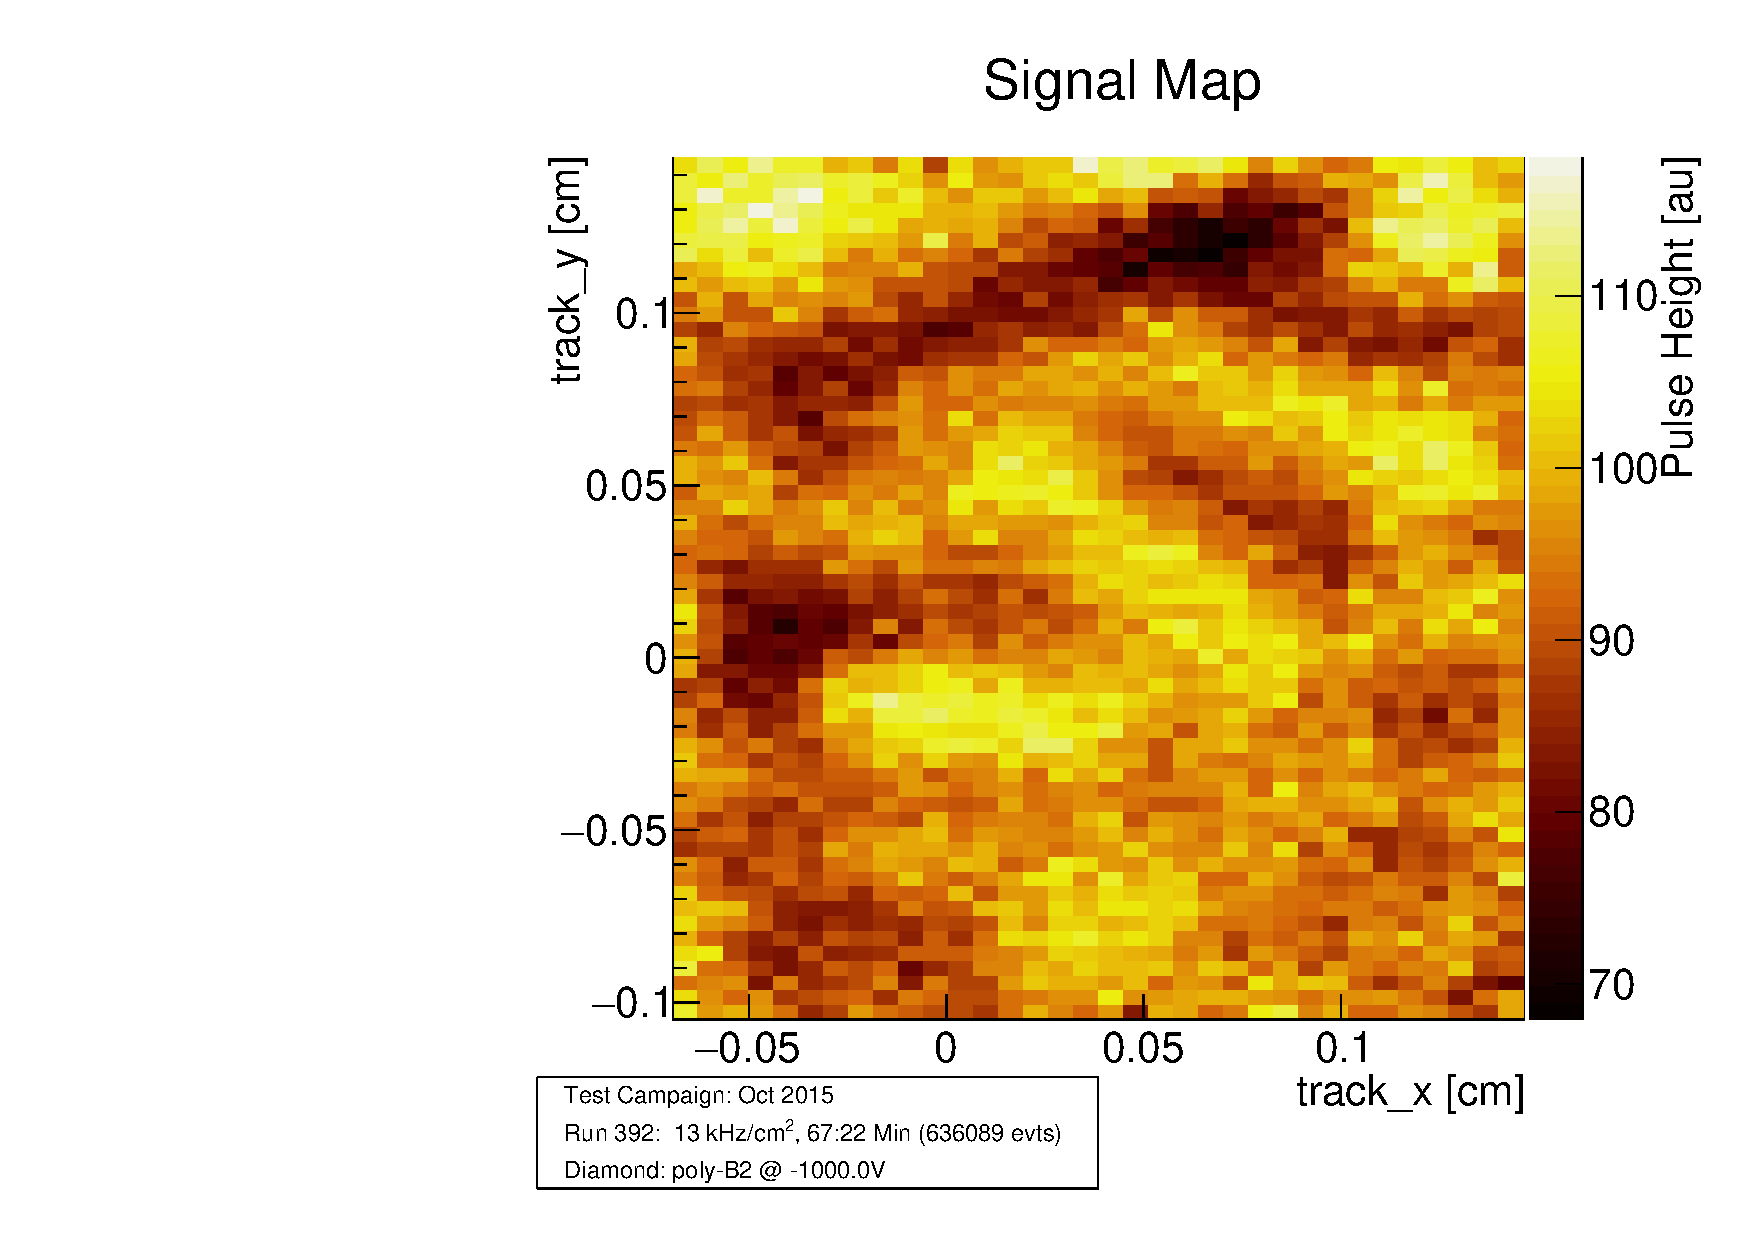
\includegraphics[angle=270, width=3.1cm]{SM392}
	\end{minipage}
	\hspace*{2pt}
	\begin{minipage}{3.1cm}
		\centering
		August 2016 - \SI[exponent-product = \cdot]{1e15}{n/cm^{2}}
		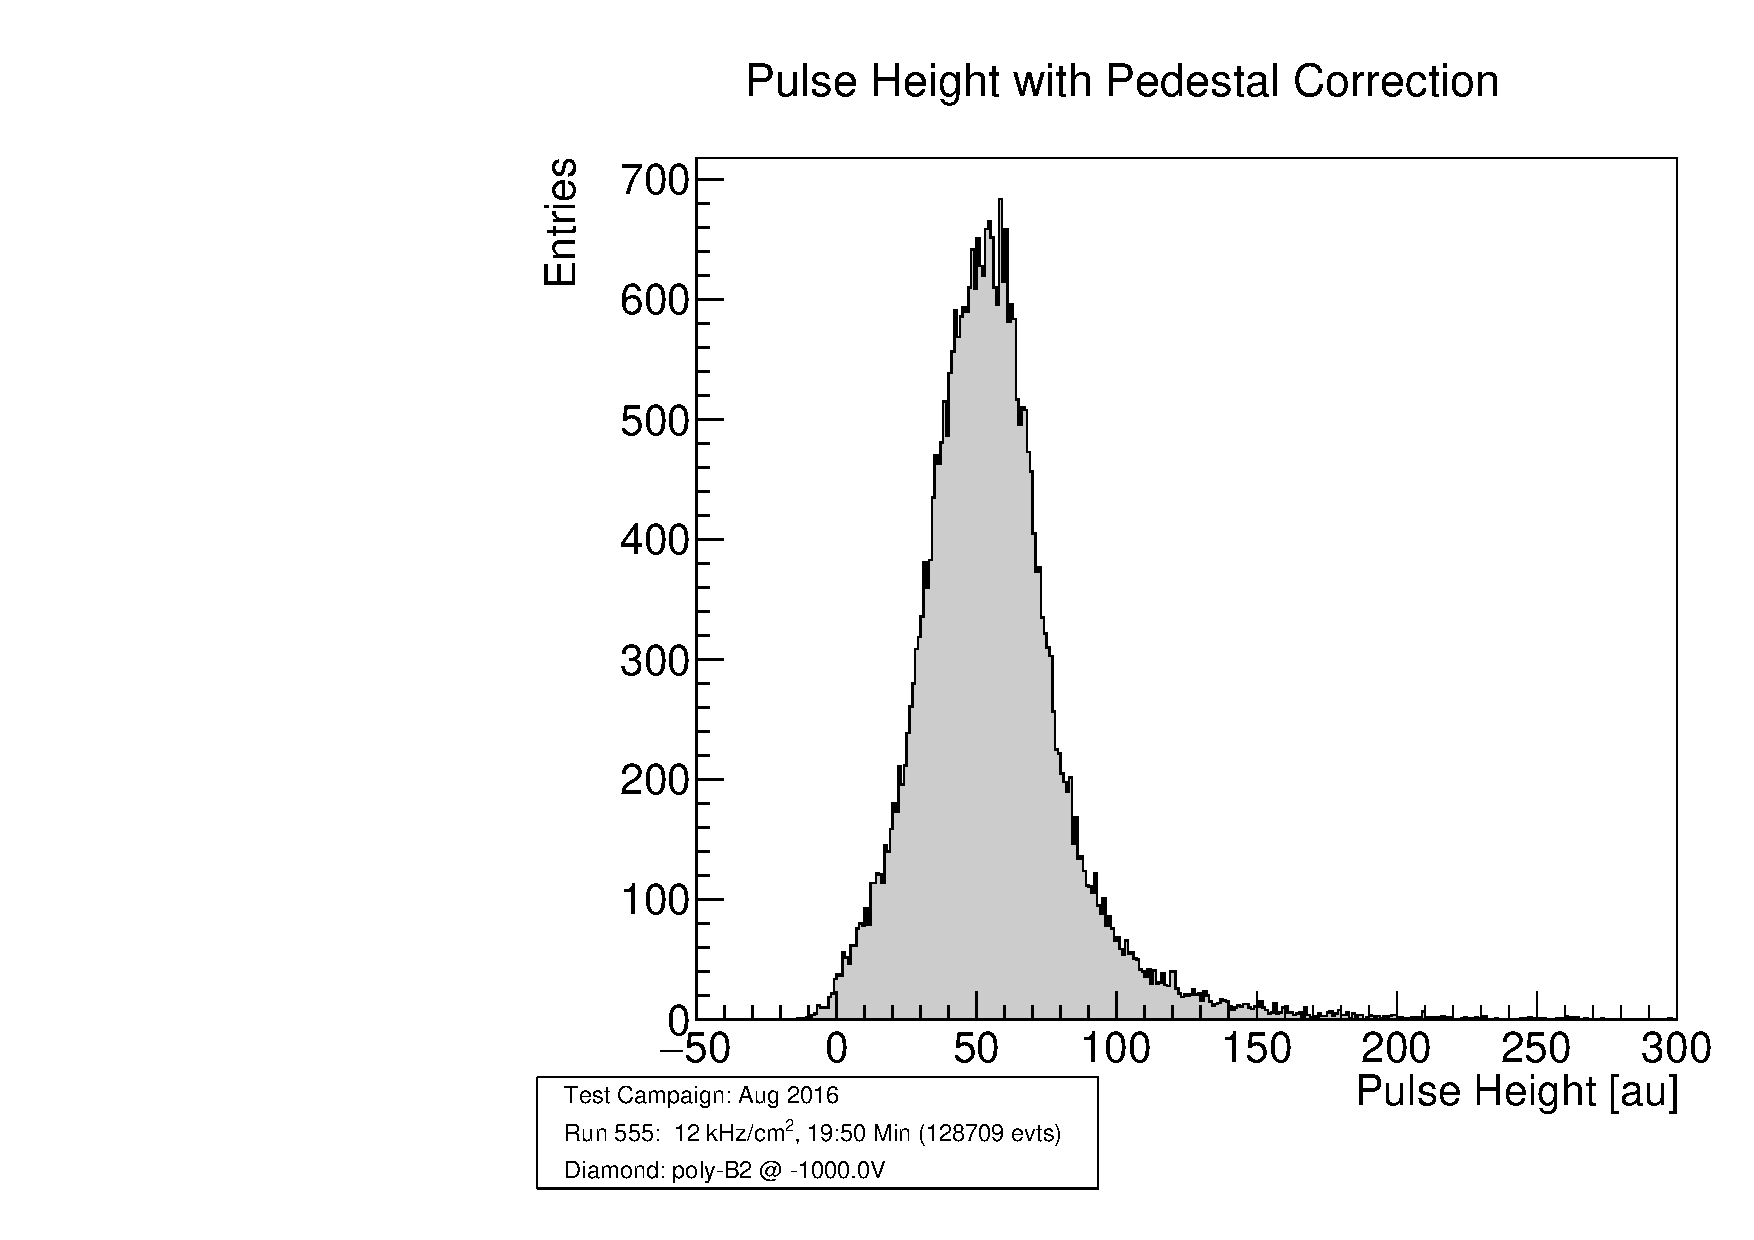
\includegraphics[angle=270, width=3.1cm]{SD555}\\
		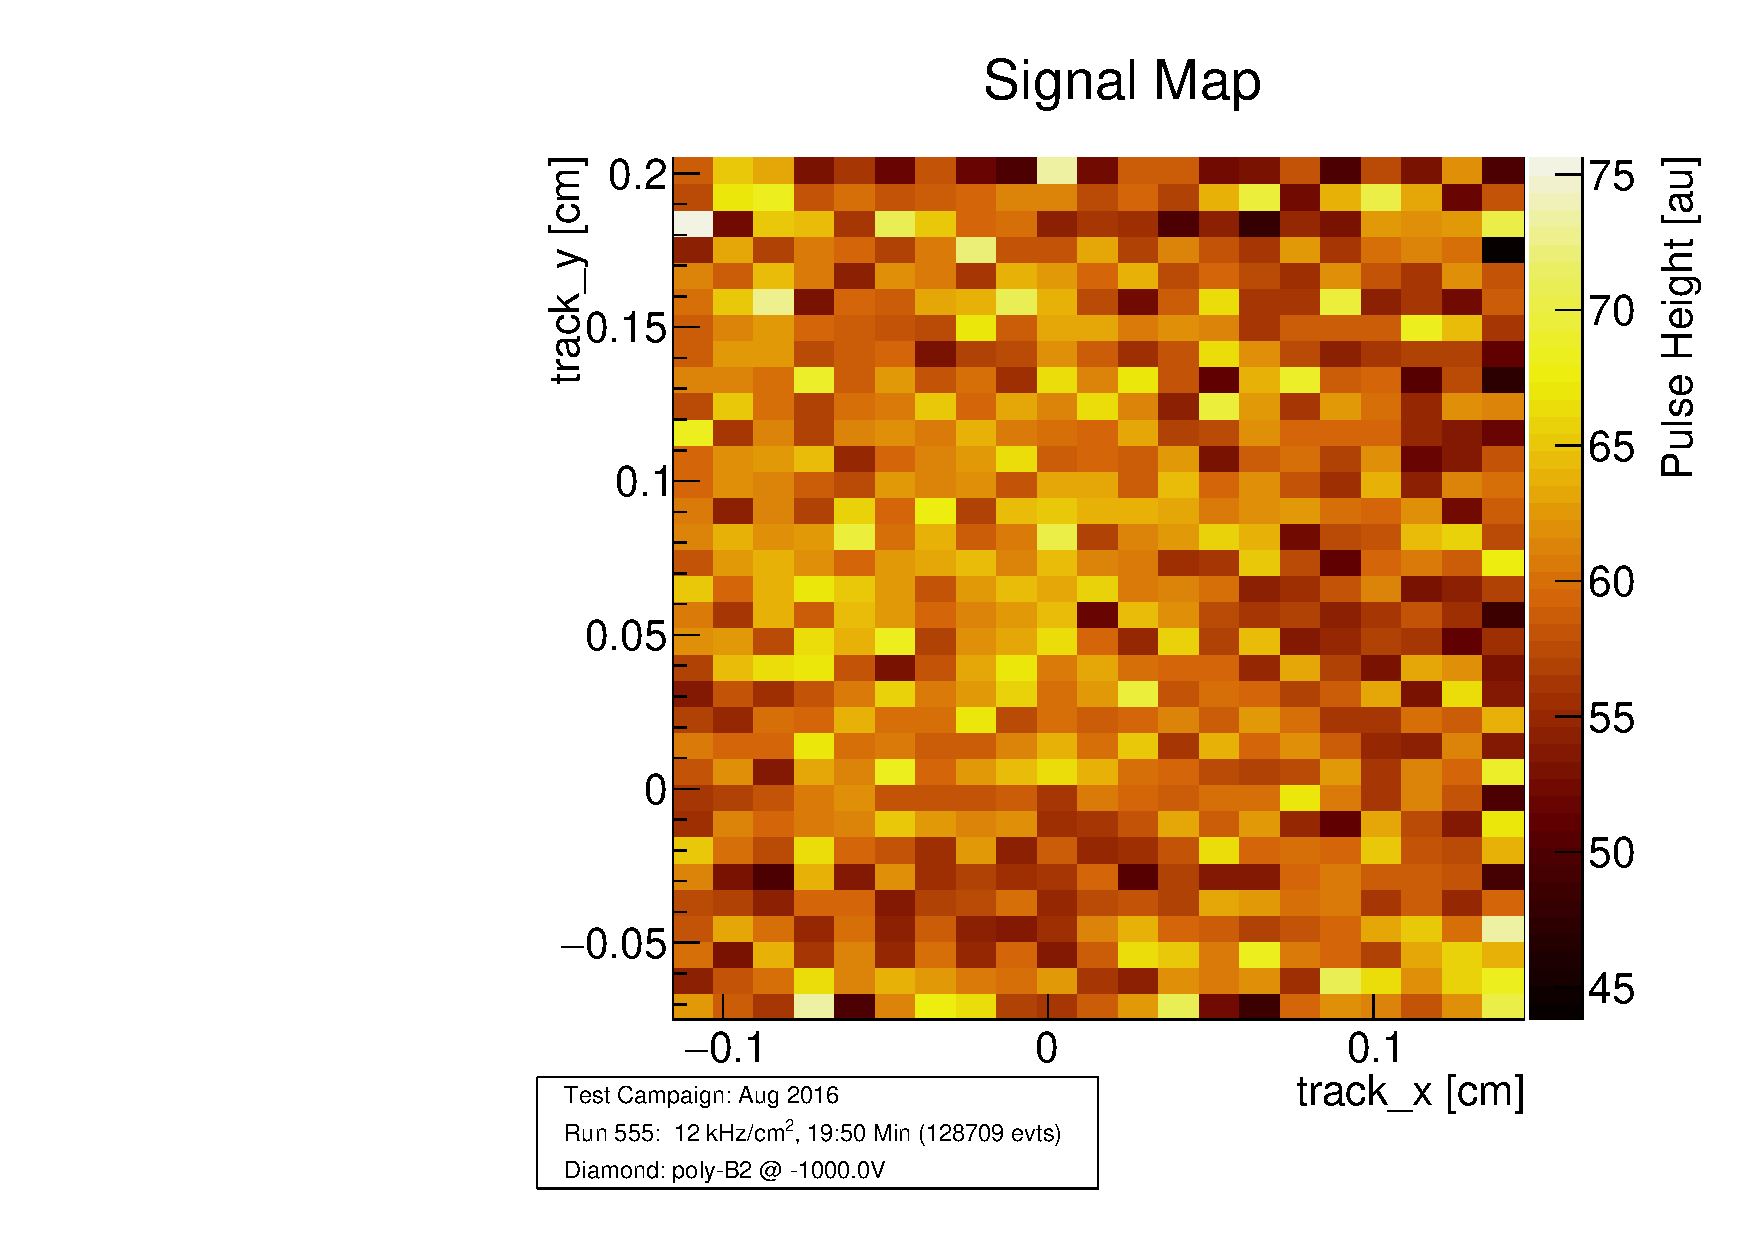
\includegraphics[angle=270, width=3.1cm]{SM555}
	\end{minipage}\s
\end{frame}
% ============================ new frame ==========================================>
\begin{frame}
	\frametitle{3D Multi Pad}
	\begin{itemize}
		\item \SI{500}{\micro\meter} thick poly-crystalline diamond sensor
		\item 25 3D cells ganged together into a single readout (quasi-pad)
	\end{itemize}
	\begin{figure}
		\centering
		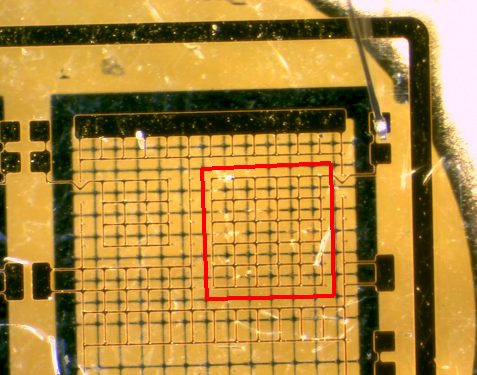
\includegraphics[width=6cm]{3DPhoto}
	\end{figure}
\end{frame}
% ============================ new frame ==========================================>
\begin{frame}
	\frametitle{3D Multi Pad - Signal Maps}
	\begin{figure}
		\centering
		\begin{subfigure}[t]{0.45\textwidth}
			\centering
			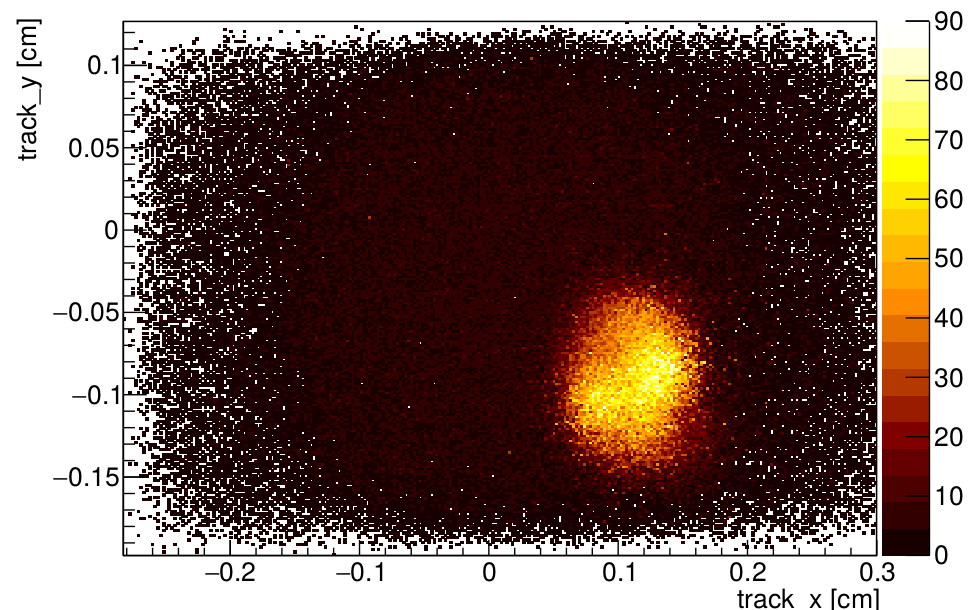
\includegraphics[width=5cm]{3DMap}
% 			\caption{blue: Diamond peak. Orange and black: Graphitic material}
		\end{subfigure}
		\begin{subfigure}[t]{0.45\textwidth}
			\centering
			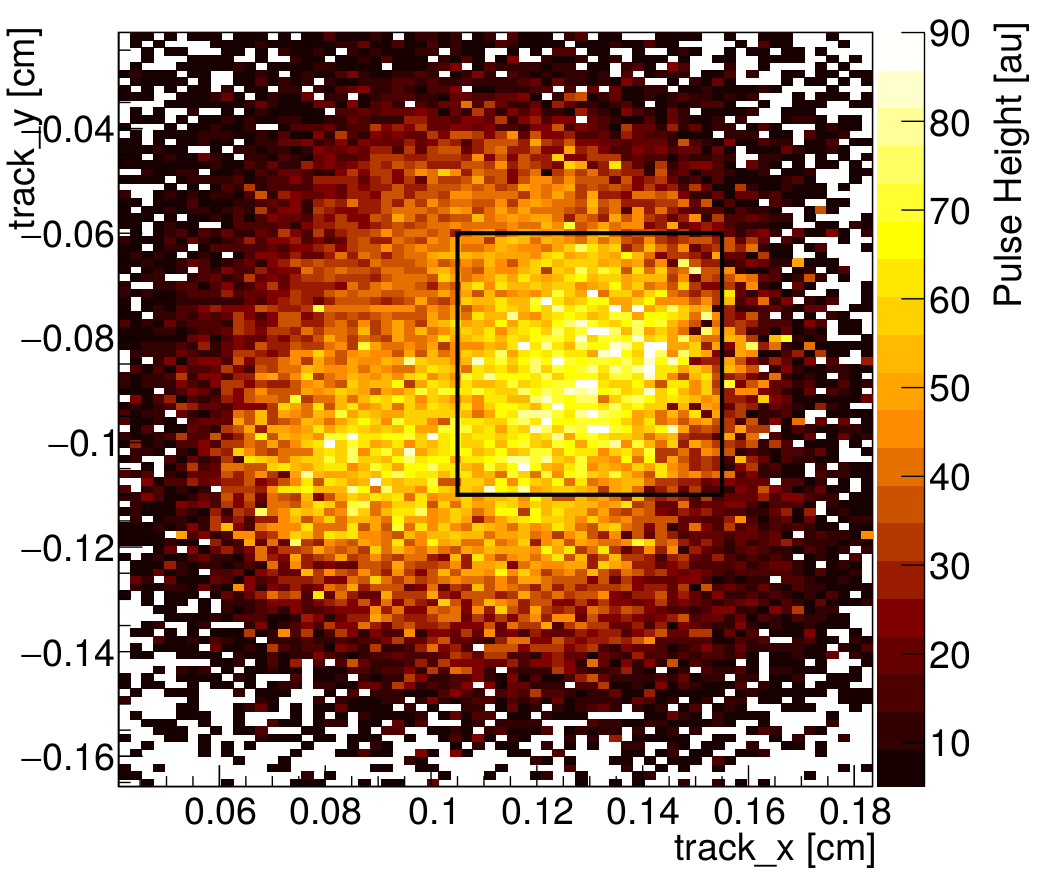
\includegraphics[height=5cm]{3DMapZoom}
% 			\caption{square and hexagonal bias patterns (red) and readout channels (blue).}
		\end{subfigure}
	\end{figure}
\end{frame}
% ============================ new frame ==========================================>
\begin{frame}
	\frametitle{3D Multi Pad - Pulse Height}
	\begin{figure}
		\centering
		\begin{subfigure}[t]{0.45\textwidth}
			\centering
			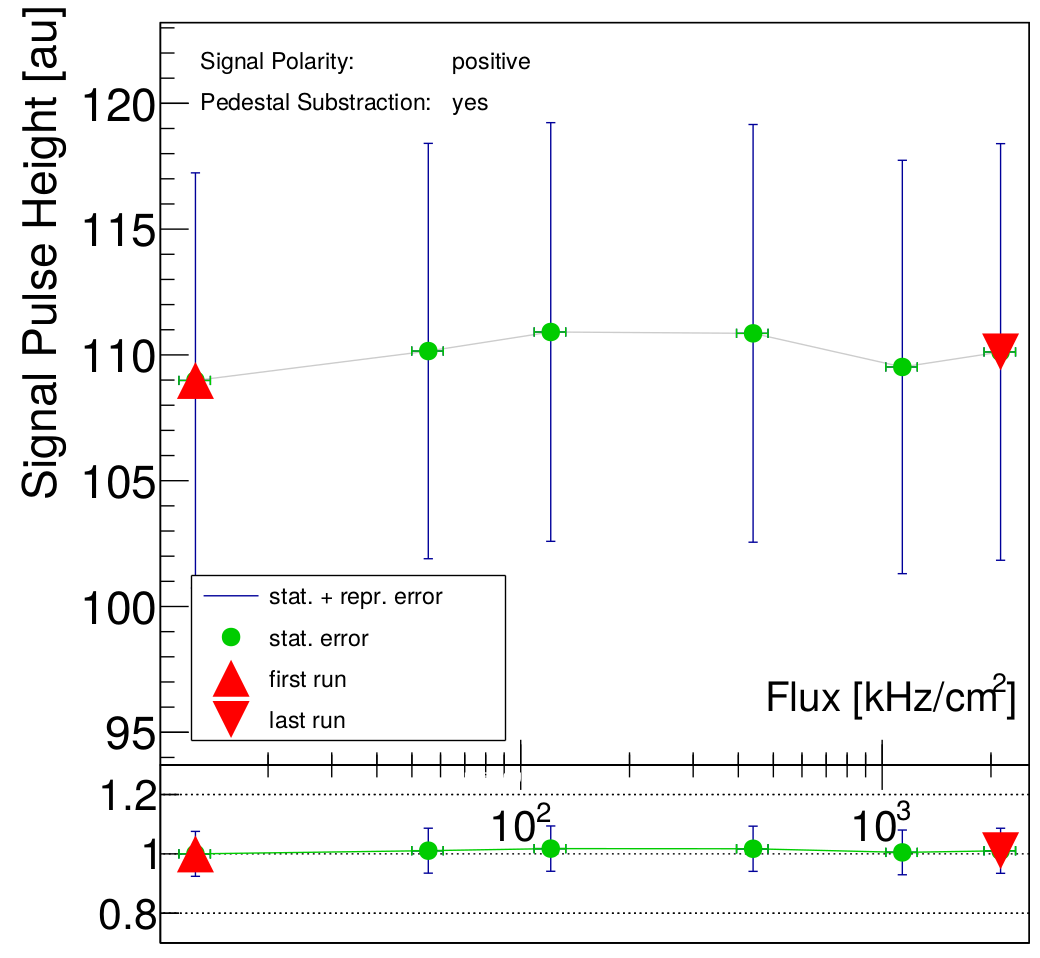
\includegraphics[height=5cm]{SiDPH}
			\caption{\SI{100}{\micro\meter} silicon diode}
		\end{subfigure}
		\begin{subfigure}[t]{0.45\textwidth}
			\centering
			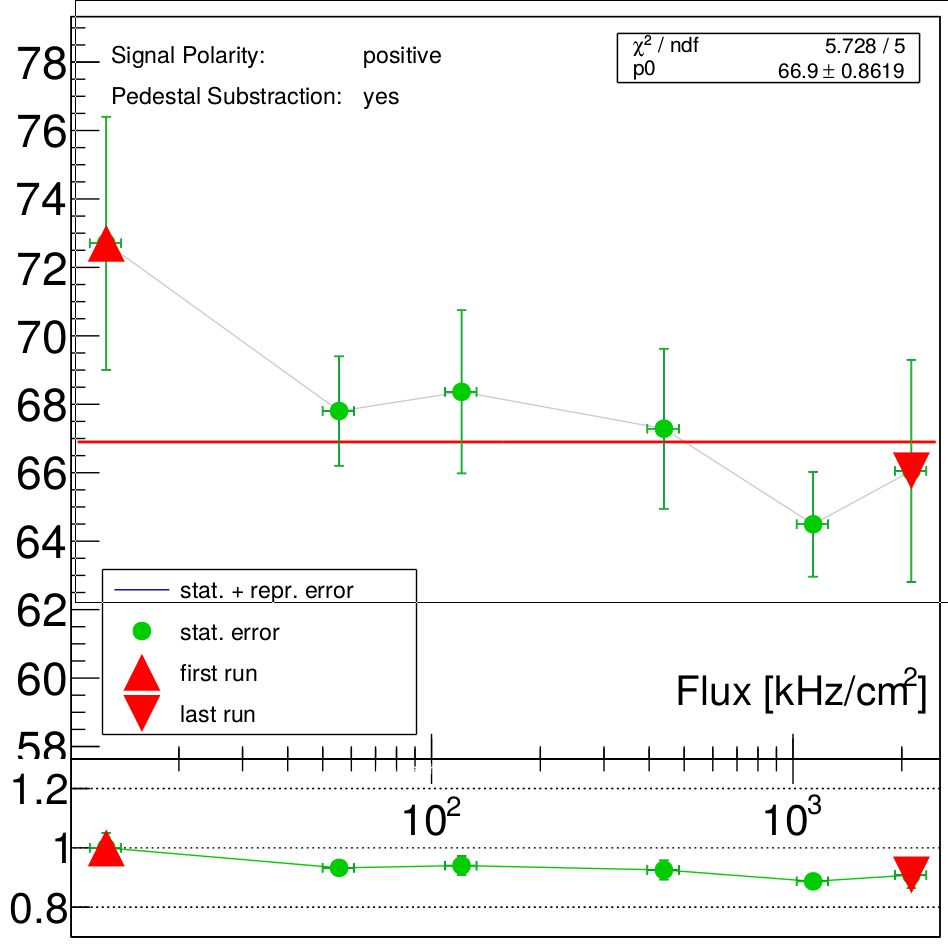
\includegraphics[height=5cm]{3DPH}
			\caption{\SI{500}{\micro\meter} poly-crystalline diamond}
		\end{subfigure}
	\end{figure}
\end{frame}
% ============================ new frame ==========================================>
\begin{frame}
	\frametitle{Reasons for Low Pulse Height}
	\begin{figure}
		\centering
		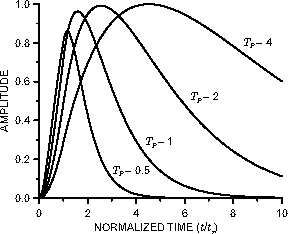
\includegraphics[width=5cm]{BallisticDeficit}
	\end{figure}
\end{frame}
% END
